\documentclass[12pt,a4paper]{report}

% --- Encoding and fonts ---
\usepackage[utf8]{inputenc}
\usepackage[T1]{fontenc}
\usepackage{mathptmx}          % Times New Roman

% --- Page geometry ---
\usepackage[margin=2.54cm]{geometry}

% --- Line spacing ---
\usepackage{setspace}
\onehalfspacing
\onehalfspacing
\setlength{\parindent}{1.25cm}
\setlength{\parskip}{0pt}

% --- Graphics ---
\usepackage{graphicx}
\usepackage{subcaption}
\usepackage{caption}
\usepackage{float}

\usepackage{tikz}
\usepackage{pgf-pie}
\usetikzlibrary{decorations.pathreplacing, positioning}

\usepackage{indentfirst}
\usepackage{enumitem}
\usepackage{amsmath}
\usepackage{microtype}
\usepackage[htt]{hyphenat}

% --- Tables ---
\usepackage{booktabs}
\usepackage{array}
\usepackage{tabularx}
\usepackage{multirow}
\usepackage{float}
\usepackage{longtable}
\usepackage{caption}
\usepackage{graphicx}
\usepackage{enumitem}
\usepackage{indentfirst}
\usepackage{titlesec}
\usepackage{ltablex}
\keepXColumns

\usepackage[table]{xcolor}

\definecolor{cellyes}{HTML}{EAF3DE}   
\definecolor{cellyesborder}{HTML}{3B6D11} 
\definecolor{cellno}{HTML}{F4F4F2}    
\definecolor{rowhdr}{HTML}{F7F7F5}    
\definecolor{colhdr}{HTML}{2C2C2A}    

\usepackage{pgfplots}
\pgfplotsset{compat=1.18}

\usepackage{pgfplotstable}

\newcommand{\Yes}{\cellcolor{cellyes}\textcolor{cellyesborder}{\textbf{+}}}
\newcommand{\No}{\cellcolor{cellno}\textcolor{gray}{---}}


% --- Paragraph formatting ---
\usepackage{indentfirst}
\setlength{\parindent}{1.25cm}
\setlength{\parskip}{6pt}

% --- Enumeration ---
\usepackage{enumitem}

% --- Hyperlinks (clickable citations) ---
\usepackage[
  colorlinks  = true,
  linkcolor   = black,
  citecolor   = black,
  urlcolor    = blue,
  pdfborder   = {0 0 0}
]{hyperref}

% --- Heading formatting ---
\usepackage{titlesec}

%   Chapter: "Chapter N. Title" - 14pt bold, centered
\titleformat{\chapter}[block]
  {\normalfont\fontsize{14}{16.8}\bfseries}
  {Chapter~\thechapter.~}{0em}{}
\titlespacing*{\chapter}{0pt}{0pt}{24pt}

%   Section (1.1, 1.2 ...): 14pt bold, flush left
\titleformat{\section}
  {\normalfont\fontsize{14}{16.8}\bfseries}
  {\thesection}{1em}{}
\titlespacing*{\section}{0pt}{18pt}{8pt}

%   Subsection (1.1.1 ...): 14pt bold italic, flush left
\titleformat{\subsection}
  {\normalfont\fontsize{14}{16.8}\bfseries\itshape}
  {\thesubsection}{1em}{}
\titlespacing*{\subsection}{0pt}{14pt}{6pt}

\captionsetup{font=small, labelfont=bf, justification=justified, singlelinecheck=false}

\pagestyle{plain}
% --- Bibliography label ---
\renewcommand{\bibname}{Bibliography}

% ============================================================
\begin{document}
% ============================================================
\begin{titlepage}
    \centering
    
    \vspace*{0cm}
    \rule{\textwidth}{0.8pt}\par
    \vspace{0.8cm}
    {\fontsize{18}{22}\selectfont \textbf{Design of a Web Dashboard for Visualizing Road Accident Statistics and Traffic Congestion in the City of Astana}\par}
    \vspace{0.8cm}
    \rule{\textwidth}{0.8pt}\par
    
    \vspace{1.2cm}
    {\large Yelemes Bayan - ST2301 \&  Shaken Ainara - ST2303\par}
    
    \vfill
    
    
\includegraphics[width=0.28\textwidth]{aitu_logo.png}\par
    \vspace{2cm}
    
    {\large School of Intelligent Systems
\par}
    {\large Astana IT University\par}
    
    \vfill
    
    {\normalsize 6B06202 - Smart Technology\par}
    {\normalsize Supervisor: Faizullin Adil\par}
    
    \vfill
    
    {\large JUNE 2026\par}
    {\large ASTANA\par}
\end{titlepage}

\pagenumbering{roman}
\setcounter{page}{1}

% ---------------- ABSTRACT ----------------
\chapter*{Abstract}
\addcontentsline{toc}{chapter}{Abstract}


Road traffic accidents and chronic congestion represent persistent challenges in rapidly
developing urban environments, generating substantial costs to public safety, economic
productivity, and quality of life. In Astana, the capital of Kazakhstan, these challenges
are compounded by the absence of any publicly accessible, analytically capable platform
through which spatial and temporal patterns in traffic incidents can be explored. Existing
commercial navigation applications provide real-time routing assistance but do not retain
historical accident records, do not support structured data submission for research
purposes, and offer no weather-correlated or district-level analytical views.
 
This thesis presents the design and implementation of \textbf{AstanaSafe} - a
web-based dashboard for visualising traffic accident statistics and congestion
information in Astana. The system was developed following a mixed-methods research
design combining primary qualitative data collection with iterative system engineering.
Semi-structured interviews were conducted in January 2026 with 19 participants across
four stakeholder segments: transport and road infrastructure specialists, monitoring
and dispatch personnel, urban planners and academic researchers, and everyday
commuters and drivers. Interview findings confirmed that data fragmentation, the
absence of spatial visualisation tools, and the inaccessibility of historical records
are the most consistently reported barriers to effective use of traffic information
across all user groups.
 
The implemented system integrates an interactive map interface built on
OpenStreetMap via the Leaflet.js library, a crowdsourced incident reporting module
with typed metadata fields, a suite of analytical visualisations including accident
density heatmaps, hourly distribution charts, severity breakdowns by district, and
weather-correlated incident analysis, and a rule-based AI safety forecast component
providing time-of-day risk assessments and predicted danger zones. 
 
The principal contributions of the work are a unified interface for accident and
congestion analysis specifically tailored to the Astana urban environment; structured,
queryable storage of user-submitted incidents enabling longitudinal analysis;
integrated weather correlation as an analytical dimension absent from all reviewed
commercial platforms; and a fully open-source architecture eliminating licensing
barriers for future research and educational deployment.
 
\vspace{0.5cm}
\noindent\textbf{Keywords:} traffic accident visualisation, road safety dashboard,
urban traffic analysis, interactive web map, crowdsourced incident reporting,
geospatial data, Astana, Kazakhstan, FastAPI, React.js


\clearpage

% ---------------- LISTS ----------------
\addcontentsline{toc}{chapter}{List of Tables}
\listoftables
\clearpage

\addcontentsline{toc}{chapter}{List of Figures}
\listoffigures
\clearpage

\tableofcontents
\clearpage

% ---------------- MAIN TEXT ----------------
\chapter*{Introduction}
\addcontentsline{toc}{chapter}{Introduction}

Urban road safety and traffic management have emerged as defining challenges of contemporary city governance. As populations grow and vehicle ownership rates rise, traffic accidents and chronic congestion pose mounting threats to public health, economic productivity, and quality of everyday life. The World Health Organization estimates that road traffic crashes claim approximately 1.19~million lives annually, representing the leading cause of death among individuals aged 5 to 29 years globally \cite{who2023}. Within this context, Astana faces a distinctive set of challenges. Since its designation as the national capital in 1997, the city has undergone rapid demographic and spatial expansion, substantially increasing vehicle ownership, introducing new arterials and intersections, and intensifying the interaction of pedestrian, private, and commercial traffic throughout the urban core.

Despite this growth, the tools available to citizens, researchers, and local authorities for monitoring road conditions remain predominantly static. Accident data is aggregated into annual administrative reports, congestion is tracked informally through navigation applications, and no publicly accessible analytical platform exists for exploring the spatial or temporal patterns that characterise road conditions across the city \cite{kzstat2023}. This gap is the central motivating problem of the present project: stakeholders including transport specialists, dispatch personnel, academic researchers, and everyday commuters are forced to rely on fragmented, non-interactive data sources, resulting in misallocated infrastructure resources, reduced situational awareness in emergency response, and significant barriers to academic work on Astana's road environment.

The present work addresses this problem through the design and implementation of \textbf{AstanaSafe} - a web-based dashboard for the visualisation of traffic accident statistics and congestion information in Astana. The system integrates an interactive map built on OpenStreetMap via the Leaflet.js library, a suite of analytical charts providing temporal, spatial, and meteorological perspectives on incident data, a crowdsourced reporting module through which authenticated users can submit and explore traffic incidents in real time, and an AI-powered safety forecast component that translates the current dataset into actionable risk assessments for different times of day and city districts. The technical stack is composed entirely of open-source components: FastAPI for the backend, React.js for the frontend, SQLite for data persistence, and the Open-Meteo API for weather data integration. This choice was made deliberately to maximise the system's accessibility, reproducibility, and extensibility for future research and development.

\textbf{Structure of the thesis.} The work is organised as follows. Chapter~1 establishes the theoretical and analytical foundation of the project: it defines the subject area and object of study, examines the problems of road accidents and traffic congestion in urban environments with specific reference to Astana, reviews the relevant academic literature and conducts a comparative analysis of existing systems, and presents the research methodology including the semi-structured interview study and its findings. Chapter~2 documents the practical development of the system: it specifies functional and non-functional requirements, describes the system architecture and technology stack, presents the implementation of each major module -- the dashboard, reporting system, analytics suite, AI forecast component, and account management -- and reports the results of functional testing. Chapter~3 outlines a structured programme of proposed improvements to be addressed in future development cycles, covering enhancements to classification granularity, map interaction, machine learning integration, administrative functionality, data quality control, and platform extensibility.

\clearpage

\pagenumbering{arabic}
\setcounter{page}{1}

\chapter{Problem Statement and Analytical Part}

% -----------------------------------------------------------
\section{Description of the Subject Area and Object of the Study}
% -----------------------------------------------------------

Urban transportation networks are among the most consequential and
technically complex components of modern city infrastructure.
As cities expand and vehicle ownership rates rise, the demands placed on
road systems multiply, generating persistent challenges in the areas of
safety, efficiency, and data governance. For municipal authorities,
academic researchers, urban planners, and everyday commuters, access to
reliable, structured, and interpretable information about traffic
conditions has become not a convenience but a practical necessity for
evidence-based decision-making \cite{who2023}.

Astana, the capital of the Republic of Kazakhstan, illustrates many of
the tensions inherent in rapidly developing urban environments. Since
its designation as the national capital in 1997, the city has undergone
dramatic expansion in both population and physical footprint. Vehicle
ownership has risen sharply over the past decade, new road networks
have been constructed, and the intersection of pedestrian, private, and
commercial traffic has grown considerably more complex. Despite these
changes, the tools available to citizens, researchers, and local
authorities for analyzing road conditions remain predominantly static:
accident data is aggregated into annual administrative reports,
congestion is monitored informally through commercial navigation
applications, and no publicly accessible, integrated analytical
platform exists for exploring the spatial or temporal patterns that
characterize road conditions across the city \cite{kzstat2023}.

This project addresses that gap directly. The \textbf{subject area} of
the research spans three intersecting domains: urban traffic safety
analysis, geospatial information processing, and the design of
interactive web-based information systems. Together, these domains
define the intellectual and technical space within which the proposed
dashboard was conceived and developed.

The \textbf{object of research} is the urban traffic system and road
safety environment of Astana - encompassing patterns of accident
occurrence, congestion formation, and the contextual conditions
(meteorological, spatial, and temporal) that influence them.

The \textbf{subject of research} is the methods and approaches employed
in the web-based visual representation of traffic accident and
congestion data, with particular focus on interactivity, accessibility,
and the practical usability of the resulting system for diverse,
non-specialist users.

The \textbf{aim} of the project is to design and implement a web
dashboard for visualizing traffic accident statistics and congestion
information in Astana, integrating interactive mapping, analytical
charts, and user-submitted incident data into a coherent and accessible
interface.

To pursue this aim, the following \textbf{objectives} were defined:

\begin{enumerate}[leftmargin=2.5cm, label=\arabic*.]
  \item Analyze existing approaches to traffic accident and congestion
    visualization, identifying the shortcomings of currently available
    tools;
  \item Design the overall architecture of the system, specifying the
    responsibilities of the frontend, backend, and database components;
  \item Implement an interactive mapping interface that allows users to
    submit and explore traffic incident markers with associated metadata;
  \item Develop analytical visualizations - heatmaps, time-based
    charts, and weather-correlation displays - that extract patterns
    from aggregated user-submitted data;
  \item Conduct functional testing of the developed system and produce
    complete technical documentation.
\end{enumerate}

The primary \textbf{target users} of the system fall into three groups:
students and academic researchers who require structured traffic data
for coursework and publications; urban planners and analysts who depend
on spatial and temporal patterns to support infrastructure decisions;
and general commuters who benefit from accessible, up-to-date
information about road conditions before and during travel.

All core technologies employed in the system are open-source. The
backend is implemented using FastAPI (Python), the frontend with
React.js, the database layer with PostgreSQL, the mapping component
with OpenStreetMap via the Leaflet.js library, and weather data are
retrieved through the Open-Meteo API \cite{fastapi2024, react2024,
osm2024, leaflet2024, openmeteo2023}. This technology stack was
selected to maximize transparency, reproducibility, and extensibility
for future developers and researchers.

% -----------------------------------------------------------
\section{The Problem of Road Accidents and Traffic Congestion in Cities}
% -----------------------------------------------------------

\subsection{The Problem of Road Accidents}

Road traffic injuries represent one of the most significant and
preventable causes of death and disability worldwide. According to the
World Health Organization's Global Status Report on Road Safety
published in 2023, approximately 1.19 million people die annually as a
direct consequence of road traffic crashes, making road accidents the
leading cause of death among people aged 5 to 29 years globally
\cite{who2023}. Between 20 and 50 million additional people sustain
non-fatal injuries each year, many resulting in long-term disability
and loss of productive capacity. The economic burden of traffic
accidents is estimated at approximately three percent of gross domestic
product in most countries, with considerably higher figures in
low- and middle-income settings where road safety governance is weaker
and medical infrastructure less developed.

Within Kazakhstan, road safety remains a persistent public health and
governance concern. Data from the Bureau of National Statistics of the
Republic of Kazakhstan indicates that road traffic accidents cause
several hundred fatalities and thousands of documented injuries each
year, with urban areas consistently accounting for the largest share of
registered incidents \cite{kzstat2023}. The capital region, which
includes Astana, records a disproportionate share of these incidents
relative to its population size, driven in part by the density of
vehicle traffic on major arterials, ongoing construction activity that
frequently modifies road configurations, and the challenges of
managing pedestrian-vehicle interaction in a rapidly expanding built
environment.

A specific challenge in the Astana context is the absence of a
publicly accessible platform through which accident data can be
explored in spatial or temporal dimensions. Researchers seeking to
identify, for example, which road sections record the highest incident
rates during adverse seasonal conditions, or how accident frequencies
differ across administrative districts, encounter substantial
difficulties in accessing and working with spatially organized data
\cite{endashaw2025, salameh2024}. The methodological gap between
data existence and data accessibility is itself a meaningful
infrastructure problem, one that a well-designed visualization
dashboard can substantially narrow.

\subsection{The Problem of Traffic Congestion}

Traffic congestion arises when demand for road space at a given
location and time approaches or exceeds the capacity of that road
section, resulting in reduced travel speeds, extended journey times,
and elevated vehicle emissions. In Astana, congestion is concentrated
primarily along major radial arterials during morning and evening
peak hours, though specific bottlenecks - particularly in the central
business district and at major intersections connecting the left and
right banks of the Ishim River - can persist for extended periods
\cite{oecd2022}.

The societal costs of congestion extend considerably beyond individual
time loss. Increased fuel consumption and elevated nitrogen oxide and
particulate emissions have measurable public health consequences.
Reduced freight delivery efficiency raises operating costs for
businesses. Studies examining driver behavior under congested
conditions consistently find higher rates of aggressive driving,
abrupt braking, and risk-taking, each of which elevates accident
probability \cite{oecd2022}. Congestion and accident occurrence are
therefore not independent phenomena: a major accident on a high-capacity
road triggers secondary congestion as traffic slows around the affected
zone, while pre-existing congestion itself elevates the risk of
further incidents.

A practical obstacle to addressing congestion in Astana is the limited
availability of structured, historically organized congestion data
accessible to the public or to researchers. Unlike major metropolitan
areas in Western Europe or East Asia where traffic management centres
aggregate data from inductive loop detectors, cameras, and GPS probe
vehicles into unified platforms, many Central Asian cities still rely
primarily on navigation application overlays and informal monitoring.
The proposed dashboard addresses this gap by incorporating
user-generated congestion markers as a lightweight crowdsourcing
mechanism, an approach that has received increasing empirical support
in recent transportation research \cite{janez2022, guo2024}.

\subsection{The Role of Information Systems and Dashboards in Data Analysis}

Information systems designed for data aggregation, processing, and
visualization have become indispensable instruments of urban
management. In the domain of traffic analysis, the capacity to
transform raw incident records into interpretable patterns is a
prerequisite for evidence-based infrastructure planning and safety
policy \cite{praharaj2022}. A dashboard, as the concept is applied in
data analytics, refers to a visual interface that consolidates multiple
data streams or indicators into a single display, enabling users to
monitor key metrics and identify patterns without requiring specialized
technical expertise.

Web-based dashboards carry particular advantages in contexts where
accessibility and ease of deployment are primary design goals. Unlike
desktop applications, browser-based interfaces require no local
installation, are platform-independent, and can be updated centrally
without imposing software management burdens on end users. For a system
intended to serve academic researchers, city officials, and ordinary
commuters simultaneously, a web-based architecture is therefore both
practically appropriate and technically sound \cite{praharaj2022,
miranda2024}.

The inclusion of a geographic map component is especially important
for traffic analytics. Road accidents and congestion events are
spatially anchored phenomena - where they occur is as analytically
important as when they occur or how frequently. An interactive map
built on an open platform such as OpenStreetMap allows users to explore
incident distributions across neighborhoods, zoom into specific
streets, and overlay multiple data layers (accident markers, density
heatmaps, weather indicators) in a spatially coherent view
\cite{osm2024, salameh2024}. This kind of multi-layered spatial
visualization is simply not achievable through tabular data or
text-based reports.

Integrating weather data into a traffic analytics dashboard adds a
further analytical dimension with considerable empirical support.
Research in transportation safety has established statistically
significant associations between adverse weather conditions -
including precipitation, reduced visibility, and freezing temperatures
- and elevated accident rates \cite{becker2022, liang2023}. By
connecting weather conditions to incident records through the
Open-Meteo API, the proposed system enables users to examine whether
accident or congestion patterns in Astana correlate with meteorological
variables, a capability absent from all existing consumer-facing
traffic tools examined in this analysis.

% -----------------------------------------------------------
\section{Literature Review and Comparative Analysis of Existing Systems}
% -----------------------------------------------------------

\subsection{Review of Related Research and Works}

Academic research on web-based traffic visualization has expanded
considerably over the past five years, driven by the growing
availability of open geographic data, advances in client-side
JavaScript mapping libraries, and increasing recognition that
accessible visual tools are essential for evidence-based urban
governance. Several research strands are directly relevant to the
present project.

A first strand concerns the application of geospatial analysis methods
to road accident data. Studies published across transportation safety
journals have demonstrated that spatial clustering approaches,
including kernel density estimation - the statistical foundation of
heatmap generation - are effective at identifying high-risk zones and
informing targeted safety interventions \cite{endashaw2025,
salameh2024}. These methods have been implemented in both desktop
geographic information systems and, increasingly, in web-based
environments using open-source JavaScript libraries - a shift that has
substantially lowered the technical barrier to deploying spatial
accident analysis tools.

A second strand focuses on the design and evaluation of interactive
dashboards for transportation data. Research examining how dashboard
design choices - including layout, color scheme, level of
interactivity, and data granularity - affect users' ability to derive
actionable insights consistently finds that interactive, map-centric
interfaces outperform static reports in supporting both specialist and
non-specialist users in understanding spatial traffic patterns
\cite{praharaj2022, shu2023}. A particularly relevant finding is that
accessibility for non-technical users is achievable without sacrificing
analytical depth, provided the interface is structured around familiar
navigational metaphors such as the interactive map.

A third strand concerns the use of crowdsourced and user-generated
data in traffic monitoring. The concept of volunteered geographic
information (VGI) describes geographic data contributed by non-specialist
users as a supplement or substitute for centralized data collection,
a concept whose scope and implications have been systematically reviewed
in the literature on crisis and disaster management applications
\cite{herfort2021, tzavella2022}. In transportation contexts,
crowdsourcing-based platforms have demonstrated meaningful capacity to
provide timely situational information, particularly in areas where
dedicated monitoring infrastructure is sparse or absent. Empirical
research by Guo et al. \cite{guo2024}, examining the relationship
between community-submitted traffic reports and recorded accident
occurrence, confirmed that user-generated data captures incident
patterns with sufficient reliability to support practical monitoring
applications. Additional work by Janež et al. \cite{janez2022}
examining citizen-science approaches to traffic monitoring similarly
found that community contributions can effectively complement
conventional sensor-based data collection in areas where dedicated
infrastructure remains limited.

\subsection{Comparative Analysis of Existing Systems}

To establish the specific niche that the proposed dashboard is designed
to fill, three widely used traffic information platforms were analyzed:
2GIS, Yandex Maps, and Google Maps. These platforms were selected
because they are the most commonly used navigation and mapping
applications among the target user population in Kazakhstan, and
because they represent the current functional baseline against which
prospective users would naturally evaluate any new tool.

\textbf{2GIS} is a mapping platform originating in Russia and widely
used across Commonwealth of Independent States countries, including
Kazakhstan, where it maintains detailed urban directory coverage. The
platform provides high-quality static maps and route planning but does
not offer real-time traffic overlays, accident data visualization, or
any mechanism for users to contribute or explore incident records in a
structured analytical format. Its primary utility is directory-based
navigation rather than traffic analysis \cite{osm2024}.

\textbf{Yandex Maps} provides real-time traffic conditions for major
cities through a combination of probe vehicle data and user-submitted
incident reports. It displays traffic density as a colored road overlay
and supports basic incident type reporting. However, Yandex Maps does
not offer accident density heatmaps, historical trend analysis,
district-level or temporal filtering, or weather-correlated
visualization. The platform is designed for turn-by-turn navigation
rather than analytical exploration of traffic patterns over time.

\textbf{Google Maps} offers a broadly comparable feature set to Yandex
Maps for traffic visualization purposes. Real-time congestion is
represented through color-coded road layers, and incident reporting is
supported via the mobile application. Like its counterpart, Google Maps
provides no dedicated accident analysis functionality, does not support
historical pattern visualization, and does not enable the structured,
filterable data exploration that research and planning applications
require.

Table~\ref{tab:comparison} presents a structured comparison of these
three platforms alongside the proposed dashboard, organized by key
functional dimensions.

\renewcommand{\arraystretch}{1.45}

\begin{tabularx}{\textwidth}{|p{5.3cm}|X|X|X|p{3cm}|}

\hline
\textbf{Feature} &
\textbf{2GIS} &
\textbf{Yandex Maps} &
\textbf{Google Maps} &
\textbf{Proposed \newline Dashboard} \\
\hline
\endfirsthead

\hline
\textbf{Feature} &
\textbf{2GIS} &
\textbf{Yandex Maps} &
\textbf{Google Maps} &
\textbf{Proposed \newline Dashboard} \\
\hline
\endhead

Interactive map interface   & Yes     & Yes     & Yes     & Yes \\
\hline
Real-time traffic overlay   & No      & Yes     & Yes     & No (user markers) \\
\hline
Accident density heatmap    & No      & No      & No      & Yes \\
\hline
Analytical charts           & No      & No      & No      & Yes \\
\hline
Weather correlation view    & No      & No      & No      & Yes \\
\hline
User-submitted incidents    & No      & Partial & Partial & Yes (structured) \\
\hline
Historical pattern analysis & No      & No      & No      & Yes (via markers) \\
\hline
Filtering by type/severity  & No      & No      & No      & Yes \\
\hline
Open-source platform        & No      & No      & No      & Yes \\
\hline
No API key required for use & Partial & No      & No      & Yes \\
\hline
\caption{\centering Comparative analysis of existing traffic information systems
and the proposed dashboard}
\label{tab:comparison} \\

\end{tabularx}

The comparison reveals a consistent pattern: established platforms
offer strong real-time navigation functionality but lack the
combination of analytical depth, structured data entry, and historical
pattern exploration that characterizes the proposed system. The
conceptual distinction is significant - existing tools are navigation
assistants, while the proposed dashboard is an analytical platform
designed to support research, planning, and informed commuting
decisions.

\subsection{Novelty of the Proposed System}

Based on the comparative analysis above and the review of related
academic work, the principal contributions of the proposed dashboard
that distinguish it from existing solutions can be summarized as
follows.

First, the system provides a \textbf{unified interface} for both
accident visualization and congestion reporting specifically tailored
to the Astana urban environment, a combination that does not currently
exist in any publicly accessible tool in this geographic context.

Second, the dashboard implements \textbf{structured, queryable storage}
of user-submitted incidents with typed metadata fields - incident
category, severity level, geographic coordinates, description, date and
time, and road name - enabling longitudinal analysis that grows in
richness as the contributor base expands.

Third, the integration of \textbf{weather data via the Open-Meteo API}
allows users to examine meteorological influences on accident and
congestion patterns, an analytical dimension absent from all three
platforms analyzed above.

Fourth, all core system components are \textbf{fully open-source},
eliminating licensing barriers for educational and research deployment
and enabling future extension without commercial constraints.

Fifth, the interface is designed for \textbf{accessibility by
non-technical users}, using familiar map navigation, consistent visual
encoding, and straightforward data entry forms that require no
specialist knowledge to operate - a feature directly motivated by the
inclusion of general commuters and undergraduate students in the target
user groups.

% -----------------------------------------------------------
\section{Recommendations from the First Pre-Defense}
% -----------------------------------------------------------

The first pre-defense review, conducted by the supervising committee prior
to the submission of the current draft, identified three substantive
deficiencies in the project as it stood at that stage. Each deficiency was
accompanied by a binding recommendation for revision. The present section
documents those recommendations and describes the corrective measures
subsequently taken in response. All three issues have been fully resolved,
and the corresponding additions are accessible through the internal
cross-references provided below.

\textbf{Recommendation 1: Absence of a defined research methodology.}
The committee observed that the initial version of the chapter contained no
explicit description of the methodological approach underpinning the
empirical work. Specifically, neither the data-collection strategy nor the
rationale for the chosen instruments was articulated in a form suitable for
academic scrutiny. In response to this observation, a dedicated methodology
section was developed and incorporated into the chapter. It describes the
mixed-methods research design, justifies the selection of semi-structured
interviews as the primary data-collection instrument, and details the
participant recruitment strategy and interview protocol. The full
methodological exposition is presented in
\hyperref[sec:methodology]{Section~\ref{sec:methodology} (Research
Methodology)}.

\textbf{Recommendation 2: Absence of a project work plan.}
The committee further noted that the submitted draft provided no structured
account of how the project activities were sequenced over time, making it
impossible to assess the feasibility of the implementation schedule or the
logical progression between project phases. To address this, a detailed
five-stage work plan was prepared, specifying the title, time period, and
principal deliverables of each phase from initial stakeholder interviews
through to final documentation and defense preparation. This plan is
presented in tabular form in
\hyperref[tab:work_plan]{Table~\ref{tab:work_plan} (Project Work Plan)},
located within the Research Methodology section.

\textbf{Recommendation 3: Absence of a backend implementation.}
The technical review conducted during the pre-defense established that the
system at that point lacked a functioning server-side component, meaning
that data persistence, API routing, and business logic processing had not
yet been implemented. The committee required that a complete backend
solution be developed and documented before the final submission. This
work was subsequently carried out using the FastAPI framework for Python,
with PostgreSQL serving as the underlying relational database. The backend
architecture, including the technology selection rationale, endpoint
structure, and database integration approach, is documented in full in
\hyperref[subsec:backend]{\ref{subsec:backend}~(Backend Technology Stack)}.

Taken together, the revisions prompted by the first pre-defense have
materially strengthened the project by supplying the methodological
transparency, planning structure, and technical completeness that the
initial submission lacked. Each of the three recommendations has been
addressed in a manner consistent with the committee's stated requirements,
and the additions have been integrated into the document so as to
preserve the internal coherence of the overall argument.

\section{Research Methodology}
\label{sec:methodology}

\subsection{Methodological Approach}

The study adopts a mixed-methods research design in which qualitative
primary data collection (semi-structured interviews) is combined with
iterative system design and engineering. This approach is well
established in applied information systems research, where understanding
user requirements forms the foundation for system specification, and
where prototype validation provides empirical evidence that purely
theoretical analysis alone cannot supply. The qualitative component
addressed the research questions concerning user needs, existing data
gaps, and desired dashboard features, while the engineering component
translated those requirements into a working system.

\subsection{Semi-Structured Interviews}

Semi-structured interviews were selected as the primary data-collection
instrument because they allow the researcher to follow a predefined
topic guide while retaining the flexibility to explore unexpected
themes or particularly informative participant responses. This balance
is appropriate when the phenomenon under study is relatively
under-researched in the specific local context, as is the case with
traffic data needs in Astana, where no prior needs-assessment for a
traffic analytics dashboard was found in the reviewed literature.

Interviews were conducted in \textbf{January 2026}. Participants were
recruited purposively to represent four stakeholder segments with
distinct relationships to urban traffic data:

\begin{itemize}[leftmargin=2cm]
  \item \textbf{Segment A - City transport and road infrastructure specialists}, including
        employees and students with expertise in urban mobility and road safety policy.
  \item \textbf{Segment B - Monitoring and dispatch users}, recruited from personnel familiar
        with iKOMEK-type operations, who manage incident reports and coordinate field responses.
  \item \textbf{Segment C - Urban planners and researchers}, primarily students and faculty at
        Astana IT University who use traffic and spatial data in academic work.
  \item \textbf{Segment D - Drivers and commuters in Astana}, representing everyday road users
        who rely on traffic information for route planning.
\end{itemize}

Each interview session covered five thematic questions tailored to the participant's segment.
Topics included: current information sources and their perceived limitations; data types of
greatest importance; desired dashboard features; and the perceived utility of the proposed
system for the participant's specific use context. Sessions were conducted in a conversational
format and lasted between 15 and 30 minutes.

\subsection{Sample Composition}

A total of \textbf{19 participants} were interviewed. Figure~\ref{fig:participant_distribution} illustrates the proportional breakdown.

\begin{figure}[H]
  \centering
  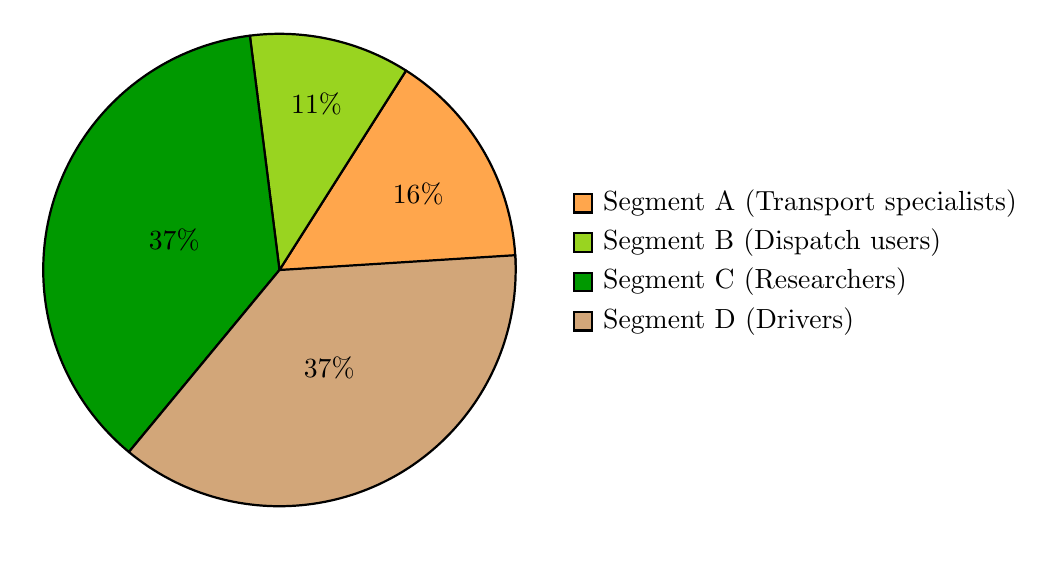
\begin{tikzpicture}
    \pie[
      text = legend,
      radius = 3,
      color = {orange!70, yellow!60!green, green!60!black, brown!70},
      before number = ,
      after number = \%
    ]{
      16/Segment A (Transport specialists),
      11/Segment B (Dispatch users),
      37/Segment C (Researchers),
      37/Segment D (Drivers)
    }
  \end{tikzpicture}
  \caption{\centering Distribution of interview participants by stakeholder segment ($n = 19$)}
  \label{fig:participant_distribution}
\end{figure}

\subsection{Interview Results}

The findings from each segment are summarised below. Demand frequency chart
(Figure~\ref{fig:feature_demand}) is provided to distil the principal cross-segment
patterns before the narrative discussion.


\begin{figure}[H]
  \hspace*{-1.5cm}
  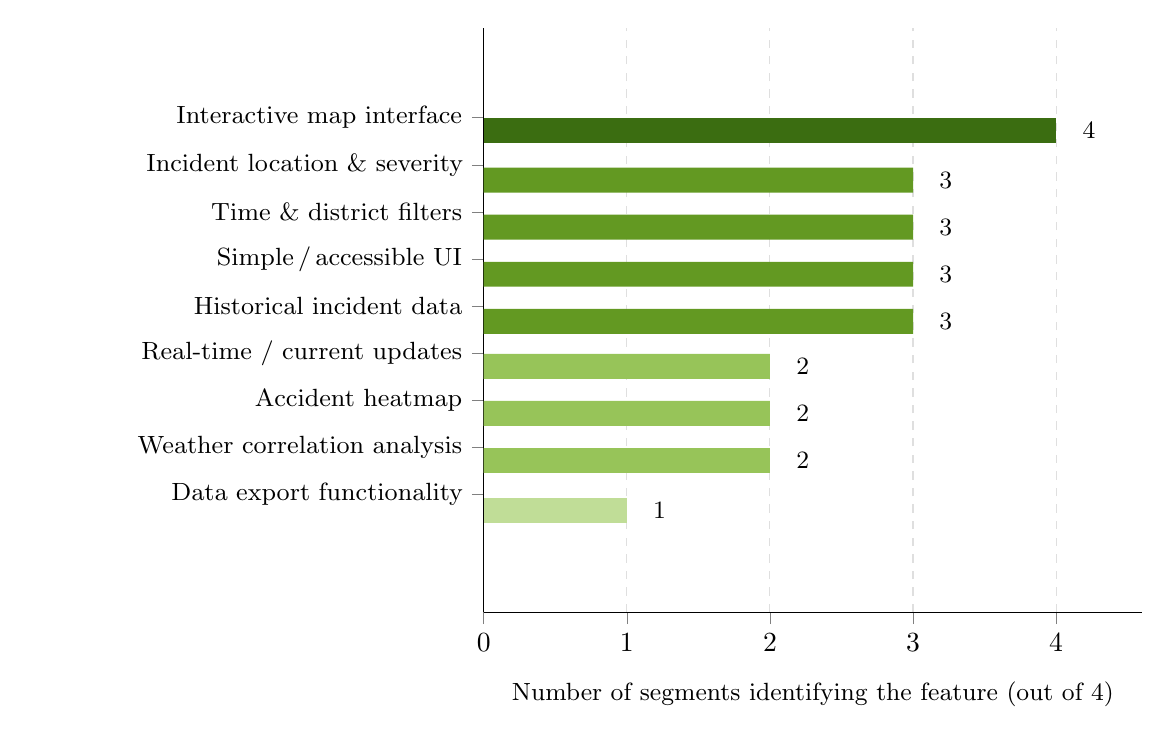
\begin{tikzpicture}
    \begin{axis}[
      xbar,
      width  = 0.82\textwidth,
      height = 9cm,
      bar width = 9pt,
      enlarge y limits = 0.12,
      xmin = 0, xmax = 4.6,
      xtick = {0,1,2,3,4},
      xlabel = {Number of segments identifying the feature (out of 4)},
      xlabel style = {font=\small, yshift=-4pt},
      ytick = {1,2,3,4,5,6,7,8,9},
      yticklabels = {
        Data export functionality,           
        Weather correlation analysis,        
        Accident heatmap,                    
        Real-time / current updates,         
        Historical incident data,            
        Simple\,/\,accessible UI,            
        Time \& district filters,            
        Incident location \& severity,       
        Interactive map interface            
      },
      yticklabel style = {font=\small, align=right, text width= 5.4cm},
      tick align = outside,
      axis x line* = bottom,
      axis y line* = left,
      xmajorgrids = true,
      grid style  = {dashed, gray!25},
      nodes near coords,
      nodes near coords align = {horizontal},
      every node near coord/.append style = {
        font=\small\bfseries,
        xshift=6pt,
        color=black
      },
      legend style = {draw=none},
    ]
      
      \addplot[fill={rgb,255:red,59;green,109;blue,17},  draw=none] coordinates {(4,9.7)};
      \addplot[fill={rgb,255:red,99;green,153;blue,34},  draw=none] coordinates {(3,8)(3,7)(3,6)(3,5)};
      \addplot[fill={rgb,255:red,151;green,196;blue,89}, draw=none] coordinates {(2,3.4)(2,2.4)(2,1.4)};
      \addplot[fill={rgb,255:red,192;green,221;blue,151},draw=none] coordinates {(1, -0.3)};
    \end{axis}
  \end{tikzpicture}
  \caption{\centering Number of stakeholder segments identifying each dashboard feature as a priority. 
           Colour encodes demand tier:
           \textcolor[RGB]{59,109,17}{\rule{9pt}{9pt}} all 4 segments;\;
           \textcolor[RGB]{99,153,34}{\rule{9pt}{9pt}} 3 segments;\;
           \textcolor[RGB]{151,196,89}{\rule{9pt}{9pt}} 2 segments;\;
           \textcolor[RGB]{192,221,151}{\rule{9pt}{9pt}} 1 segment.}
  \label{fig:feature_demand}
\end{figure}

\textbf{Segment A - Transport and road infrastructure specialists.} Respondents in this group reported obtaining traffic and accident information primarily
from open government datasets, navigation applications, official city websites, and
internal institutional reports. A recurring concern was that data is scattered across
multiple sources and is almost always presented in static formats - PDFs, spreadsheets,
or fixed-column tables - without any spatial or temporal visualisation. When asked which
data attributes matter most, all respondents highlighted accident location, time of
occurrence, severity, and congestion level as the four most critical variables. Regarding
desired features, interactive maps, accident heatmaps, filters by time period and
administrative district, and the ability to compare data across different periods
emerged as the most consistent preferences. Respondents unanimously agreed that a
dedicated analytics dashboard would strengthen evidence-based infrastructure planning
and road safety policy in the city.

\textbf{Segment B - Monitoring and dispatch users.} Participants in this segment described their current information channels as phone calls
received from citizens, internal dispatch communications, and shift reports. The central
difficulty they identified was the absence of a consolidated visual representation of
ongoing incidents: information arrives as unstructured text through multiple disconnected
channels and must be manually aggregated before it can be acted upon. The data attributes
considered most critical during operations were precise incident location, current severity
level, traffic impact on surrounding roads, and incident status (active~/ resolved). A
real-time interactive map with incident status indicators, priority flags, and category
filters was identified as the most valuable potential feature of a centralised dashboard.
All participants agreed that such a system would meaningfully improve situational awareness
and operational efficiency.

\textbf{Segment C - Urban planners and researchers.} Astana IT University students and faculty reported using traffic and accident data in the
context of coursework, research projects, and academic publications. The most commonly
cited difficulties were data fragmentation across government portals, the absence of
ready-made visualisations, and the need for extensive manual preprocessing before any
analysis can begin. Participants placed particular value on access to historical records,
interactive spatial maps, time-series charts, and data export functionality that would
allow integration with statistical tools. The proposed dashboard was viewed as a
potential time-saving resource for academic work, enabling users to move from data
access to substantive analysis without a laborious preparation phase.

\textbf{Segment D - Drivers and commuters.} Everyday road users reported relying primarily on navigation applications and, in some
cases, informal social media groups to monitor traffic conditions before and during their
commutes. Common frustrations included delayed updates, insufficient detail about accident
circumstances, and the psychological stress associated with unexpected delays. Desired
features centred on real-time congestion maps, accident alerts with route alternatives,
and clean, simple interfaces that do not require technical knowledge to interpret. The
majority of respondents indicated that they would use a web-based traffic dashboard
regularly, provided that it delivered accurate, timely, and easily understandable
information.

A structured summary of findings by stakeholder segment is presented in
Table~\ref{tab:interview_results}.

\renewcommand{\arraystretch}{1.5}

\begin{tabularx}{\textwidth}{|p{3cm}|X|X|X|}

\hline
\textbf{Segment} &
\textbf{Main Data \newline Challenges} &
\textbf{Priority Features} &
\textbf{Perceived Value} \\
\hline
\endfirsthead

\hline
\textbf{Segment} &
\textbf{Main Data \newline Challenges} &
\textbf{Priority Features} &
\textbf{Perceived Value} \\
\hline
\endhead

A - Transport \newline specialists &
Fragmented data sources, static formats, absence of spatial visualization &
Interactive map, heatmap, district-level filters, historical comparison tools &
Infrastructure planning support, data-driven road safety policy \\ 
\hline

B - Dispatch / monitoring &
Lack of centralized visual platform, manual data aggregation under time pressure &
Real-time map, severity classification, incident status filtering &
Enhanced situational awareness, faster response coordination \\ 
\hline

C - Researchers / students &
High preprocessing effort, lack of localized visualization tools, fragmented datasets &
Historical datasets, export functionality, temporal charts, spatial analysis tools &
Lower barrier to entry, effective support for academic and coursework tasks \\ 
\hline

D - Drivers / \newline commuters &
Delayed updates, insufficient incident detail, unpredictable congestion patterns &
Congestion visualization, accident alerts, intuitive user interface &
Improved trip planning, reduced uncertainty and travel stress \\ 
\hline

\caption{\centering Summary of interview findings by stakeholder segment}
\label{tab:interview_results} \\

\end{tabularx}

\subsection{Cross-Cutting Findings}

Several themes emerged consistently across all four segments and directly informed the system's
functional requirements:

\begin{enumerate}[leftmargin=2cm, label=\arabic*.]
  \item \textbf{Data fragmentation} was universally identified as the primary barrier to
        effective use of traffic information.
  \item \textbf{Spatial representation} (maps) was the most frequently requested feature,
        mentioned by every participant in every segment.
  \item \textbf{Filtering by time and category} was considered essential for both professional
        and casual use.
  \item \textbf{Simplicity of interface} was emphasised by research users and everyday drivers
        alike, indicating that the dashboard must serve non-technical audiences without
        sacrificing analytical depth.
  \item \textbf{Weather context} was spontaneously mentioned by Segment A and Segment C
        participants as an important analytical variable, independently validating the
        decision to integrate the Open-Meteo API.
\end{enumerate}

\subsection{Project Work Plan}

The project was executed in five sequential stages. Table~\ref{tab:work_plan} provides a
structured overview of each stage, its timeline, and its principal deliverables.

\renewcommand{\arraystretch}{1.4}

\begin{tabularx}{\textwidth}{|>{\centering\arraybackslash}p{0.4cm}
                  |>{\raggedright\arraybackslash}p{2.8cm}
                  |>{\centering\arraybackslash}p{4.2cm}
                  |>{\raggedright\arraybackslash}X|}


\hline
\textbf{\#} & \textbf{Stage} & \textbf{Period} & \textbf{Key Activities} \\
\hline
\endfirsthead

\hline
\textbf{\#} & \textbf{Stage} & \textbf{Period} & \textbf{Key Activities} \\
\hline
\endhead

0 & Stakeholder interviews & January 2026 &
Conduct semi-structured interviews with 19 participants across four segments;
collect and analyse user needs \\
\hline

1 & Theoretical research \& analysis & Feb 2026 - Apr 2026 &
Literature review; analysis of existing systems; definition of requirements and methodology \\
\hline

2 & System design \& planning & Feb 2026 - Apr 2026 &
Client-server architecture design; database schema; UI concept prototyping (Figma) \\
\hline

3 & System development & Mar 2026 - 20 Apr 2026 &
Frontend implementation (React, Leaflet); backend (FastAPI); API integrations (Open-Meteo, OSM); filtering and data processing \\
\hline

4 & Testing \& validation & Mar 2026 - 20 Apr 2026 &
Functional testing; UI/UX validation; filtering accuracy checks; performance evaluation \\
\hline

5 & Finalisation \& documentation & Apr 2026 - Jun 2026 &
System optimisation; technical documentation; presentation preparation; final defence \\
\hline

\caption{\centering Project work plan by stage}
\label{tab:work_plan} \\

\end{tabularx}





\setcounter{chapter}{1}
\chapter{Development of the Practical Part}

\section{System Requirements and Architecture}

\subsection{System Requirements}

The requirements for the AstanaSafe dashboard were derived from two primary sources: the literature review conducted in Chapter 1, which identified the analytical gaps in existing platforms, and the semi-structured interview study, which established the specific informational needs of each stakeholder group. Requirements were divided into functional and non-functional categories following standard software engineering practice~\cite{swebok2014}.

Functional requirements define the observable behaviours the system must support. They were prioritised using a three-tier scheme reflecting the frequency and criticality of each feature as reported during the interview study. Table~\ref{tab:func_req} presents the complete set of functional requirements.

\renewcommand{\arraystretch}{1.4}

\begin{tabularx}{\textwidth}{|>{\centering\arraybackslash}p{1.5cm}
                  |>{\raggedright\arraybackslash}X
                  |>{\centering\arraybackslash}p{1.9cm}|}

\hline
\textbf{ID} & \textbf{Requirement} & \textbf{Priority} \\
\hline
\endfirsthead

\hline
\textbf{ID} & \textbf{Requirement} & \textbf{Priority} \\
\hline
\endhead

FR-01 & Display incident markers on an interactive city map with colour-coded severity & High \\
\hline
FR-02 & Allow authenticated users to submit traffic reports via a modal form & High \\
\hline
FR-03 & Filter displayed records by district, incident type, severity, and weather & High \\
\hline
FR-04 & Present analytics charts including hourly distribution, severity by district, and weather impact & High \\
\hline
FR-05 & Provide KPI metric cards showing total incidents, high-severity ratio, peak hour, and district safety status & High \\
\hline
FR-06 & Maintain a searchable historical archive of all submitted reports with export functionality & Medium \\
\hline
FR-07 & Generate an AI-based safety forecast with time-of-day risk levels and predicted danger zones & Medium \\
\hline
FR-08 & Automatically attach weather condition data to each submitted incident record & Medium \\
\hline
FR-09 & Display a severity-weighted heatmap layer on the interactive map & Medium \\
\hline
FR-10 & Provide personal account management including contribution history and data privacy controls & Low \\
\hline

\caption{\centering Functional requirements of the AstanaSafe dashboard} \label{tab:func_req} \\

\end{tabularx}


Non-functional requirements address the system's operational qualities, including performance, security, and usability. They were defined in accordance with the ISO/IEC 25010 software quality model and with the access constraints of the intended user groups~\cite{iso25010}. Table~\ref{tab:nonfunc_req} summarises these requirements.


  \renewcommand{\arraystretch}{1.4}
  \begin{tabularx}{\textwidth}{|>{\centering\arraybackslash}p{1.6cm}
                                |>{\raggedright\arraybackslash}X
                                |>{\centering\arraybackslash}p{2.8cm}|}
    \hline
    \textbf{ID} & \textbf{Requirement} & \textbf{Category} \\
    \hline
    NFR-01 & The dashboard must be accessible via a standard web browser without installation & Accessibility \\
    \hline
    NFR-02 & Initial page load time must not exceed three seconds under standard network conditions & Performance \\
    \hline
    NFR-03 & The interface must be usable by non-technical users without specialist training & Usability \\
    \hline
    NFR-04 & User authentication must protect submitted data using hashed credentials & Security \\
    \hline
    NFR-05 & All submitted incident records must persist across sessions in a relational database & Reliability \\
    \hline
    NFR-06 & The system must support cross-origin requests from the frontend domain & Compatibility \\
    \hline
    NFR-07 & The codebase must use exclusively open-source, licence-free components & Maintainability \\
    \hline

  \caption{\centering Non-functional requirements of the AstanaSafe dashboard}
  \label{tab:nonfunc_req}
  
  \end{tabularx}
  


\subsection{System Architecture and Design}

AstanaSafe follows a client-server web application architecture, in which the browser-based frontend and the Python API backend operate as separate processes communicating via a REST interface. This separation of concerns simplifies independent development and testing of each layer and allows the frontend to be served as a static bundle while the backend handles all data logic~\cite{praharaj2022}.

Table~\ref{tab:arch_layers} presents the four architectural layers of the system and their respective components.


  \renewcommand{\arraystretch}{1.4}
  \begin{tabularx}{\textwidth}{|>{\raggedright\arraybackslash}p{2.6cm}
                                |>{\raggedright\arraybackslash}p{3.7cm}
                                |>{\raggedright\arraybackslash}X|}
    \hline
    \textbf{Layer} & \textbf{Components} & \textbf{Responsibilities} \\
    \hline
    Presentation layer & React (Vite), Leaflet, Chart.js & Renders all UI components, map tiles, charts, and forms in the browser \\
    \hline
    Application layer & FastAPI, Uvicorn, Pydantic & Exposes REST endpoints, validates request/ response data, executes business logic \\
    \hline
    Data layer & SQLAlchemy ORM, SQLite & Persists and queries incident records, user accounts, and district data \\
    \hline
    External services & Open-Meteo API, OpenStreetMap tiles & Provides current weather data and base map raster tiles \\
    \hline
    
\caption{\centering Architectural layers of the AstanaSafe system}
  \label{tab:arch_layers}
  \end{tabularx}
  

Communication between the frontend and backend follows a standard REST API pattern using JSON-formatted payloads. CORS middleware is enabled on the backend to allow requests originating from the frontend development server. Table~\ref{tab:api_endpoints} lists the primary API endpoints implemented in the system.

\renewcommand{\arraystretch}{1.4}

\begin{tabularx}{\textwidth}{|>{\centering\arraybackslash}p{2cm}
                  |>{\raggedright\arraybackslash}p{4cm}
                  |>{\raggedright\arraybackslash}X|}


\hline
\textbf{Method} & \textbf{Endpoint} & \textbf{Description} \\
\hline
\endfirsthead

\hline
\textbf{Method} & \textbf{Endpoint} & \textbf{Description} \\
\hline
\endhead


GET & /api/accidents & Retrieve all accident records \\
\hline

GET & /accidents/heatmap & Retrieve severity-weighted coordinates for heatmap rendering \\
\hline

GET & /api/traffic-reports & Retrieve all user-submitted traffic reports \\
\hline

POST & /traffic-reports & Submit a new traffic or accident report \\
\hline

DELETE & /traffic-reports/\{id\} & Remove a specific report by identifier \\
\hline

GET & /api/roads/districts & Retrieve GeoJSON district boundary data \\
\hline

GET & /api/ai/forecast & Retrieve the AI-generated safety forecast for the current date \\
\hline

\caption{\centering Primary REST API endpoints of the AstanaSafe backend} \label{tab:api_endpoints}

\end{tabularx}


The interface prototyping phase used Figma to develop layout concepts and design prototypes, which were then refined into the final component structure implemented in React. The overall layout follows a sidebar-plus-topbar pattern with a card-based main content area, a structure identified in the interface requirements study as intuitive for non-technical users.

\section{Selection and Description of Development Technologies}

\subsection{Frontend Technology Stack}

The frontend is implemented as a single-page application (SPA) built on React, a component-based JavaScript library maintained by Meta Open Source~\cite{react2024}. The SPA architecture eliminates full-page reloads when navigating between views, reducing latency and preserving map state across route transitions - an important consideration for a dashboard where the map is the central element. Vite serves as the build tool and development server, providing fast hot module replacement during development and optimised bundle output for production~\cite{vitejs2024}.

Client-side routing between the five main pages - Dashboard, Analytics, Reports, AI Forecast, and My Account - is managed by \texttt{react-router-dom}, which maps URL paths to component trees without requiring server-side routing logic. Map rendering is handled by Leaflet through the \texttt{react-leaflet} wrapper library, which exposes Leaflet's functionality as declarative React components and renders tiles from the OpenStreetMap tile server~\cite{leaflet2024, osm2024}. Chart.js, integrated through \texttt{react-chartjs-2}, drives all analytical visualisations, including line graphs, donut charts, stacked bar charts, and horizontal bar rankings~\cite{chartjs2024}. Zustand provides lightweight global state management through the \texttt{useAppStore} hook, storing the currently selected date, active filters, and fetched report data. HTTP communication with the backend uses an Axios-style API client that wraps fetch calls in a consistent interface. The icon system is supplied by \texttt{lucide-react}.

Table~\ref{tab:frontend_stack} summarises the complete frontend dependency set.

\renewcommand{\arraystretch}{1.4}

\begin{tabularx}{\textwidth} {|p{5.5cm}
                  |p{2.5cm}
                  |X|}


\hline
\textbf{Library / Tool} & \textbf{Version} & \textbf{Purpose} \\
\hline
\endfirsthead

\hline
\textbf{Library / Tool} & \textbf{Version} & \textbf{Purpose} \\
\hline
\endhead

React & 18.2.0 & Core UI component framework \\
\hline
Vite & 5.2.0 & Build tool and development server \\
\hline
react-router-dom & 6.22.3 & Client-side routing between pages \\
\hline
Leaflet / react-leaflet & 1.9.4 / 4.2.1 & Interactive map rendering \\
\hline
Chart.js / react-chartjs-2 & 4.4.1 / 5.2.0 & Analytics chart visualisations \\
\hline
Zustand & 4.5.2 & Global application state management \\
\hline
Axios (client abstraction) & 1.6.7 & REST API communication \\
\hline
react-datepicker & 4.21.0 & Global and page-level date selection \\
\hline
lucide-react & 0.383.0 & Icon system \\
\hline

\caption{\centering Frontend technology stack}
\label{tab:frontend_stack} \\

\end{tabularx}

\subsection{Backend Technology Stack}
\label{subsec:backend}

The backend is built with FastAPI, a modern Python web framework designed for high-performance API development~\cite{fastapi2024}. FastAPI generates automatic OpenAPI documentation from type annotations, which simplified endpoint testing during development. The ASGI server Uvicorn runs the FastAPI application and handles concurrent connections. Request and response models are validated by Pydantic, which enforces schema compliance at the boundary between client and server and converts incoming JSON payloads into typed Python objects~\cite{pydantic2024}. Database interaction is abstracted through SQLAlchemy's ORM layer, which maps Python class definitions to relational database tables~\cite{sqlalchemy2024}.

The backend project is organised into the following modules: \texttt{main.py} serves as the application entry point and configures CORS middleware; \texttt{models.py} defines the SQLAlchemy database models; \texttt{schemas.py} contains the Pydantic request and response schemas; and the \texttt{routers/} directory groups endpoint definitions by entity, including \texttt{accidents.py} and \texttt{traffic\_reports.py}.

\subsection{Database Design and Schema}

The system uses SQLite as the local development database, stored in the file \texttt{astanasafe.db}. The decision to defer PostGIS integration was made on the basis of complexity reduction: geospatial district assignment is handled entirely on the frontend through a custom helper function, \texttt{getDistrictForPoint(lat, lng, geojson)}, which evaluates submitted coordinates against loaded GeoJSON district boundary polygons. This approach eliminates a backend dependency while preserving spatial functionality.

The database schema comprises four tables. Table~\ref{tab:schema_accidents} describes the \texttt{accidents} table, which stores seeded and imported incident records.

\renewcommand{\arraystretch}{1.4}

\begin{tabularx}{\textwidth}{|p{3.0cm}
                  |p{3 cm}
                  |X|}


\hline
\textbf{Column} & \textbf{Type} & \textbf{Description} \\
\hline
\endfirsthead

\hline
\textbf{Column} & \textbf{Type} & \textbf{Description} \\
\hline
\endhead

id & INTEGER & Auto-incrementing primary key \\
\hline
latitude & FLOAT & Geographic latitude of the incident \\
\hline
longitude & FLOAT & Geographic longitude of the incident \\
\hline
date & DATETIME & Recorded timestamp of the incident \\
\hline
type & VARCHAR & Incident type (collision, pedestrian, rollover) \\
\hline
severity & VARCHAR & Severity level (low, medium, high) \\
\hline
weather & VARCHAR & Weather condition at the time of incident \\
\hline
district & VARCHAR & City district name \\
\hline
description & TEXT & Optional free-text description \\
\hline

\caption{\centering Database schema: \texttt{accidents} table}
\label{tab:schema_accidents} \\

\end{tabularx}


Table~\ref{tab:schema_reports} describes the \texttt{traffic\_reports} table, which stores user-generated submissions in real time.

\renewcommand{\arraystretch}{1.4}

\begin{tabularx}{\textwidth}{|p{2.7cm}
                  |p{2.9cm}
                  |X|}


\hline
\textbf{Column} & \textbf{Type} & \textbf{Description} \\
\hline
\endfirsthead

\hline
\textbf{Column} & \textbf{Type} & \textbf{Description} \\
\hline
\endhead

id & INTEGER & Auto-incrementing primary key \\
\hline
lat & FLOAT & Latitude of the submitted report \\
\hline
lng & FLOAT & Longitude of the submitted report \\
\hline
road & VARCHAR & Selected road name \\
\hline
crossroad & VARCHAR & Selected intersection name \\
\hline
category & VARCHAR & Incident category (Active Traffic Jam, Low / Medium / High Severity) \\
\hline
type & VARCHAR & Incident type (collision, pedestrian, rollover) \\
\hline
weather & VARCHAR & Weather condition at submission time \\
\hline
district & VARCHAR & Derived district name via GeoJSON lookup \\
\hline
user\_name & VARCHAR & Display name of the submitting user \\
\hline
user\_id & INTEGER & Foreign key referencing the \texttt{users} table \\
\hline
created\_at & DATETIME & Automatic submission timestamp \\
\hline

\caption{\centering Database schema: \texttt{traffic\_reports} table}
\label{tab:schema_reports} \\

\end{tabularx}

Table~\ref{tab:schema_users} describes the \texttt{users} table, which stores authenticated user accounts.

\renewcommand{\arraystretch}{1.4}

\begin{tabularx}{\textwidth}{|p{3.5cm}
                  |p{3 cm}
                  |X|}


\hline
\textbf{Column} & \textbf{Type} & \textbf{Description} \\
\hline
\endfirsthead

\hline
\textbf{Column} & \textbf{Type} & \textbf{Description} \\
\hline
\endhead

id & INTEGER & Auto-incrementing primary key \\
\hline
name & VARCHAR & User display name \\
\hline
email & VARCHAR & Registered email address \\
\hline
phone & VARCHAR & Contact number \\
\hline
hashed\_password & VARCHAR & Bcrypt-hashed authentication credential \\
\hline
google\_sub & VARCHAR & Google OAuth 2.0 subject identifier \\
\hline
created\_at & DATETIME & Account registration timestamp \\
\hline

\caption{\centering Database schema: \texttt{users} table}
\label{tab:schema_users} \\

\end{tabularx}

A separate \texttt{districts} table stores the names of the six administrative districts of Astana covered by the system: Almaty, Baikonur, Esil, Nura, Saryarka, and Sarayshyq. This table is referenced during reporting and filtering operations to ensure consistent district labelling across all records.

\section{Implementation of the Information System}

\subsection{Dashboard and Interactive Map}

The Dashboard page is the primary entry point to the system and serves as the central monitoring screen where users access live incident data, submit reports, view district statistics, and inspect recent activity. The page layout consists of a persistent left sidebar for navigation, a topbar containing the page title, a global date picker, and the submission button, four KPI summary cards, a large map panel with filter controls, and two right-side panels for recent activity and district statistics.

The date picker in the topbar synchronises all dashboard data to a single selected day. For the test session shown in the screenshots, the selected date is April 20, 2026. The four KPI cards display the following values for that date: Total Reports: 12; Active Jams: 3; Weather: 13$^\circ$C, Cloudy, Astana; and an AI Safety Forecast card indicating a MEDIUM RISK level. The AI Safety Forecast card contains a brief executive summary generated from current report data, followed by a recommendation box advising users to reduce speed, increase following distance, and exercise particular caution in Esil district during evening and night periods.

The interactive map is rendered using Leaflet with OpenStreetMap tile layers and displays all reports as colour-coded circular markers: red for high-severity accidents, orange for medium severity, blue for low severity, and purple for active traffic jams~\cite{leaflet2024, osm2024}. A map legend in the lower-left corner of the map panel explains the colour scheme. The filter row above the map exposes three dropdown controls - All Districts, All Types, and All Weather - and a dynamic badge in the upper-right corner of the panel indicates the number of currently visible reports. For the test session, 12 reports are shown. District boundaries are drawn on the map as coloured polygon overlays loaded from a GeoJSON file.

The Recent Activity panel on the right side of the screen displays the most recent submissions in a timestamped timeline, showing incident category, road name, type, weather, submitting user, and timestamp for each entry. Below it, the District Reports panel presents per-district report counts visualised with proportional progress bars, showing Esil at 8, Nura at 1, Baikonur at 1, Saryarka at 2, Almaty at 0, and Sarayshyq at 0.

Figure~\ref{fig:dashboard} shows the Dashboard page with all components populated for April 20, 2026.

\begin{figure}[H]
  \centering
  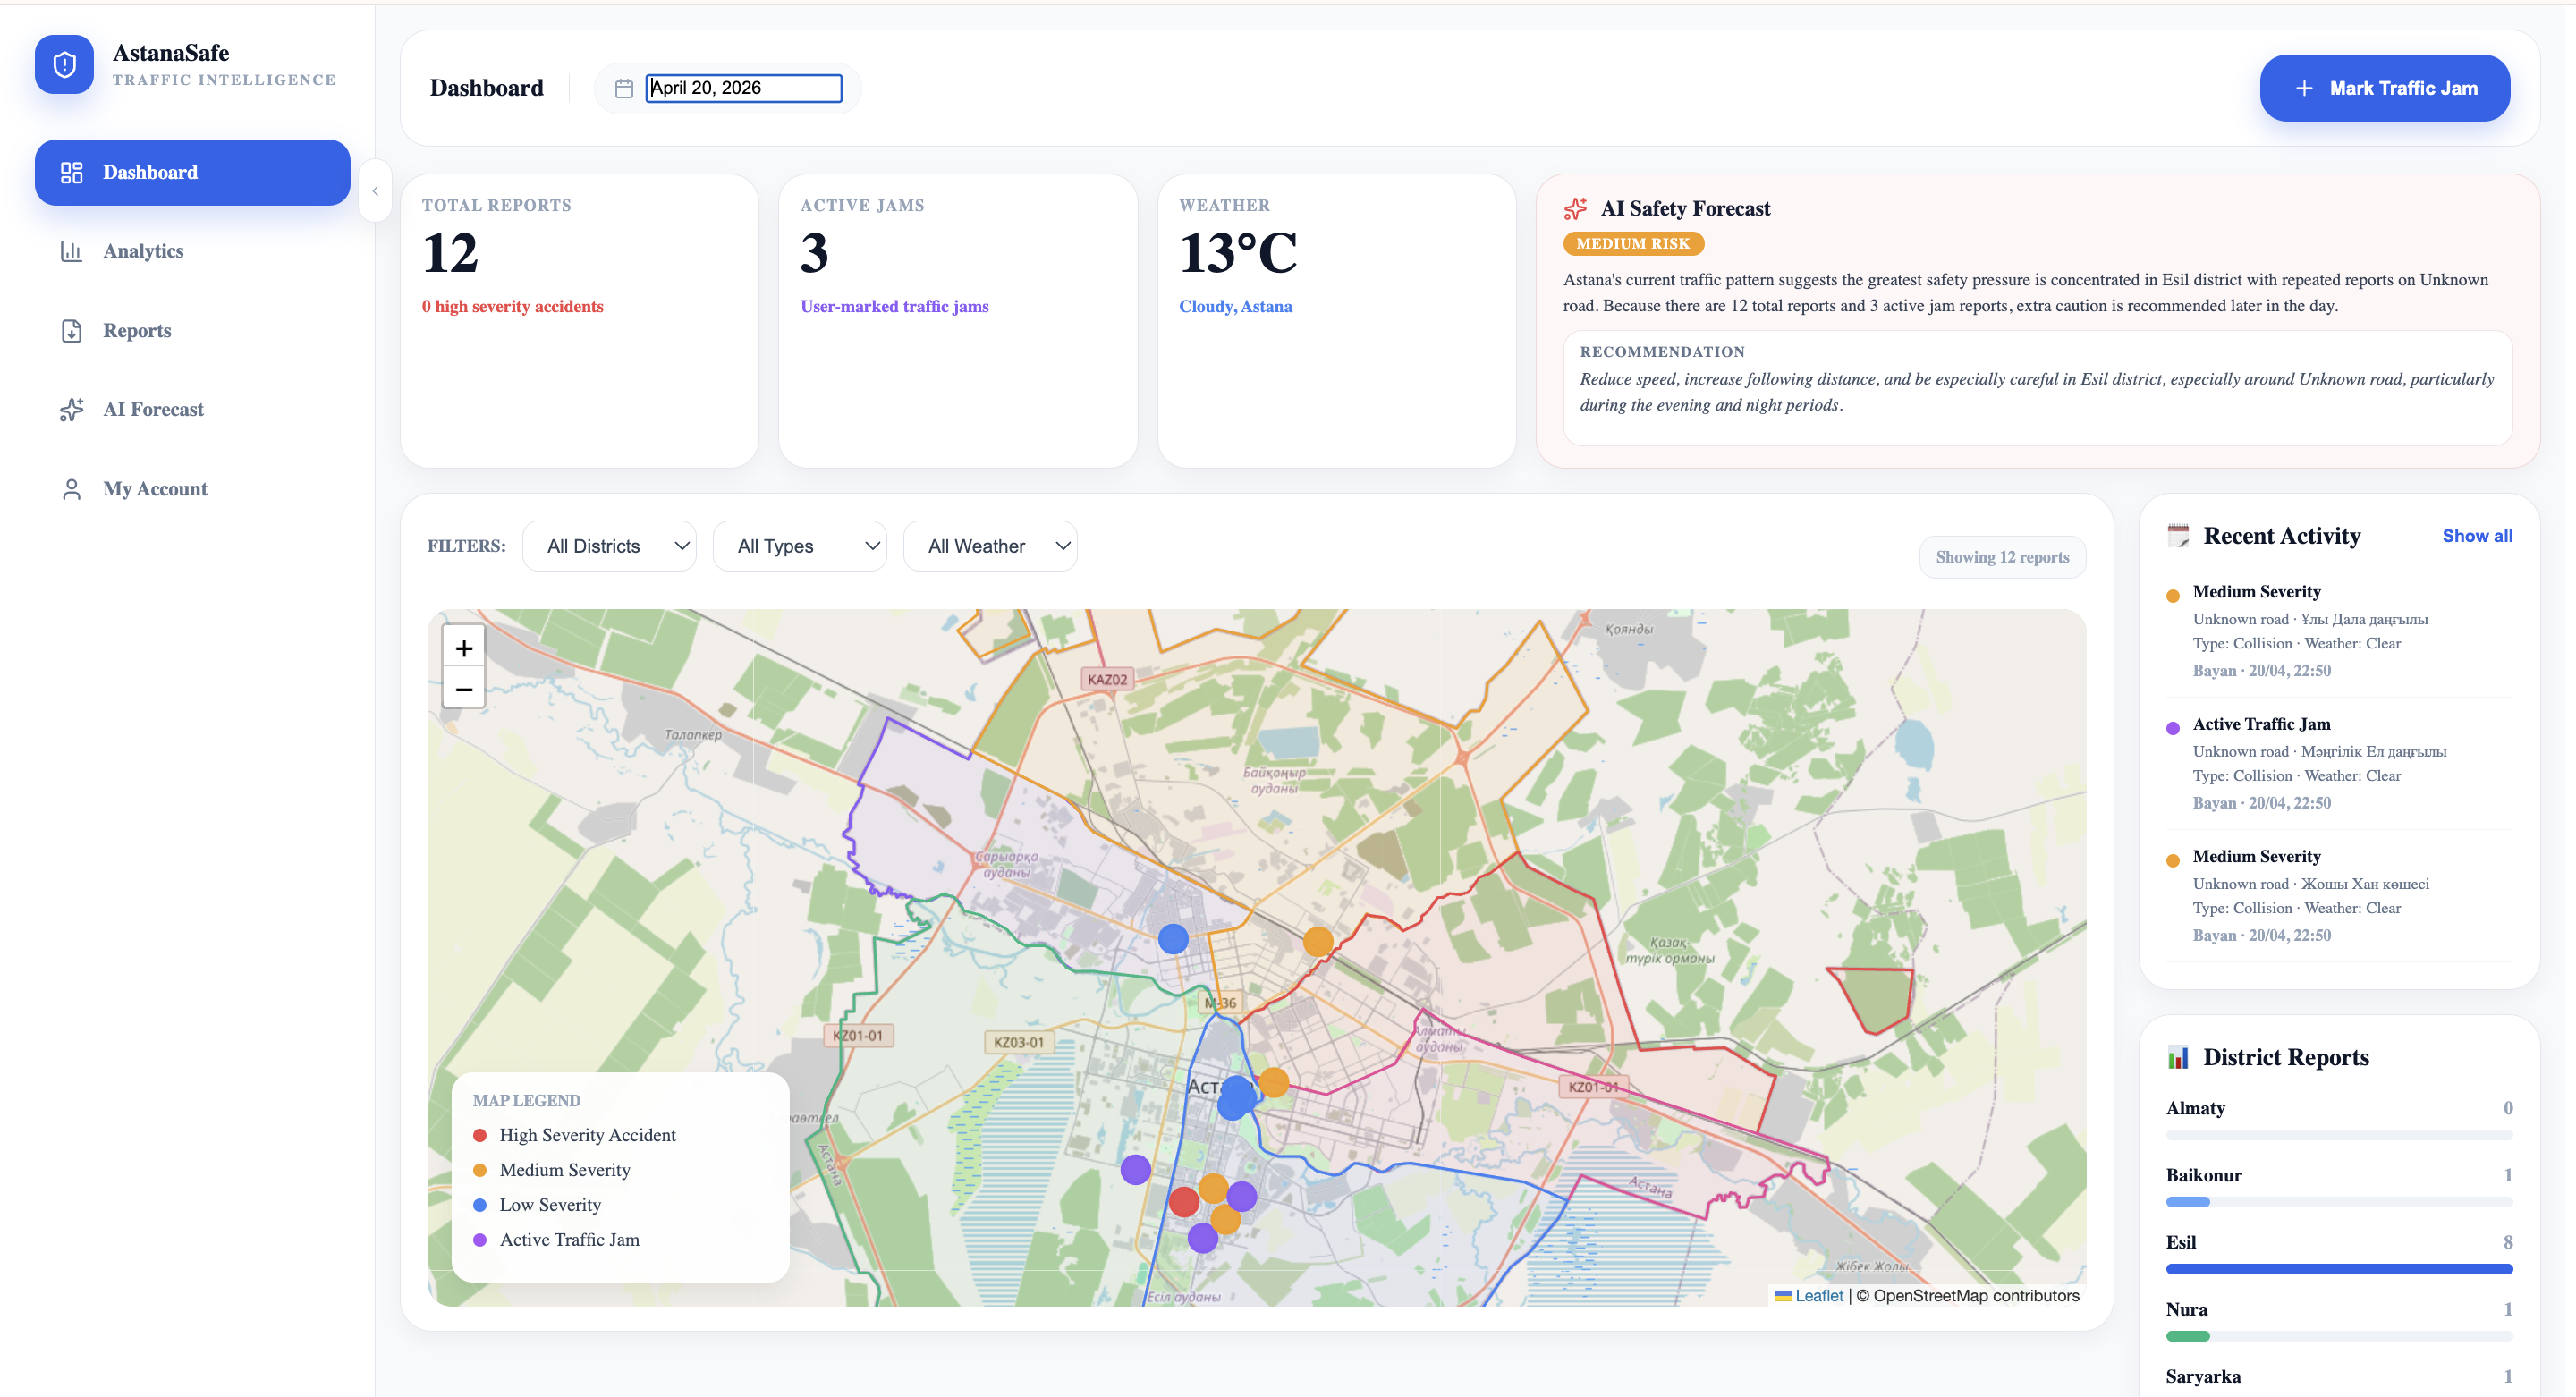
\includegraphics[width=\textwidth]{sc1_dashboard.png}
  \caption{\centering AstanaSafe Dashboard page: KPI cards, interactive map with incident markers, Recent Activity panel, and District Reports panel}
  \label{fig:dashboard}
\end{figure}

\subsection{Incident Reporting and Filtering System}

\textbf{Mark Traffic Jam modal.} Users can submit a new incident report at any time by clicking the blue Mark Traffic Jam button in the topbar. This opens a centred modal overlay above the current page. The form contains the following fields: a Select Road dropdown populated from the road database, a Crossroads / Intersection dropdown that becomes enabled once a road is selected, an Incident Category selector with four mutually exclusive options (Active Traffic Jam, Low Severity, Medium Severity, High Severity Accident), a Type dropdown (Collision, Pedestrian, Rollover), and a Weather dropdown. An informational notice below the form reads: "Your report will be pinned to the selected location and visible to all users in real-time." Submitting the form dispatches a POST request to the \texttt{/traffic-reports} endpoint, which stores the record with an automatic timestamp and the weather condition fetched from the Open-Meteo API at that moment~\cite{openmeteo2023}. The district is determined client-side by evaluating the submitted road coordinates against the GeoJSON polygon set. Figure~\ref{fig:mark_jam} shows the open modal for the Mark Traffic Jam action.

\begin{figure}[H]
  \centering
  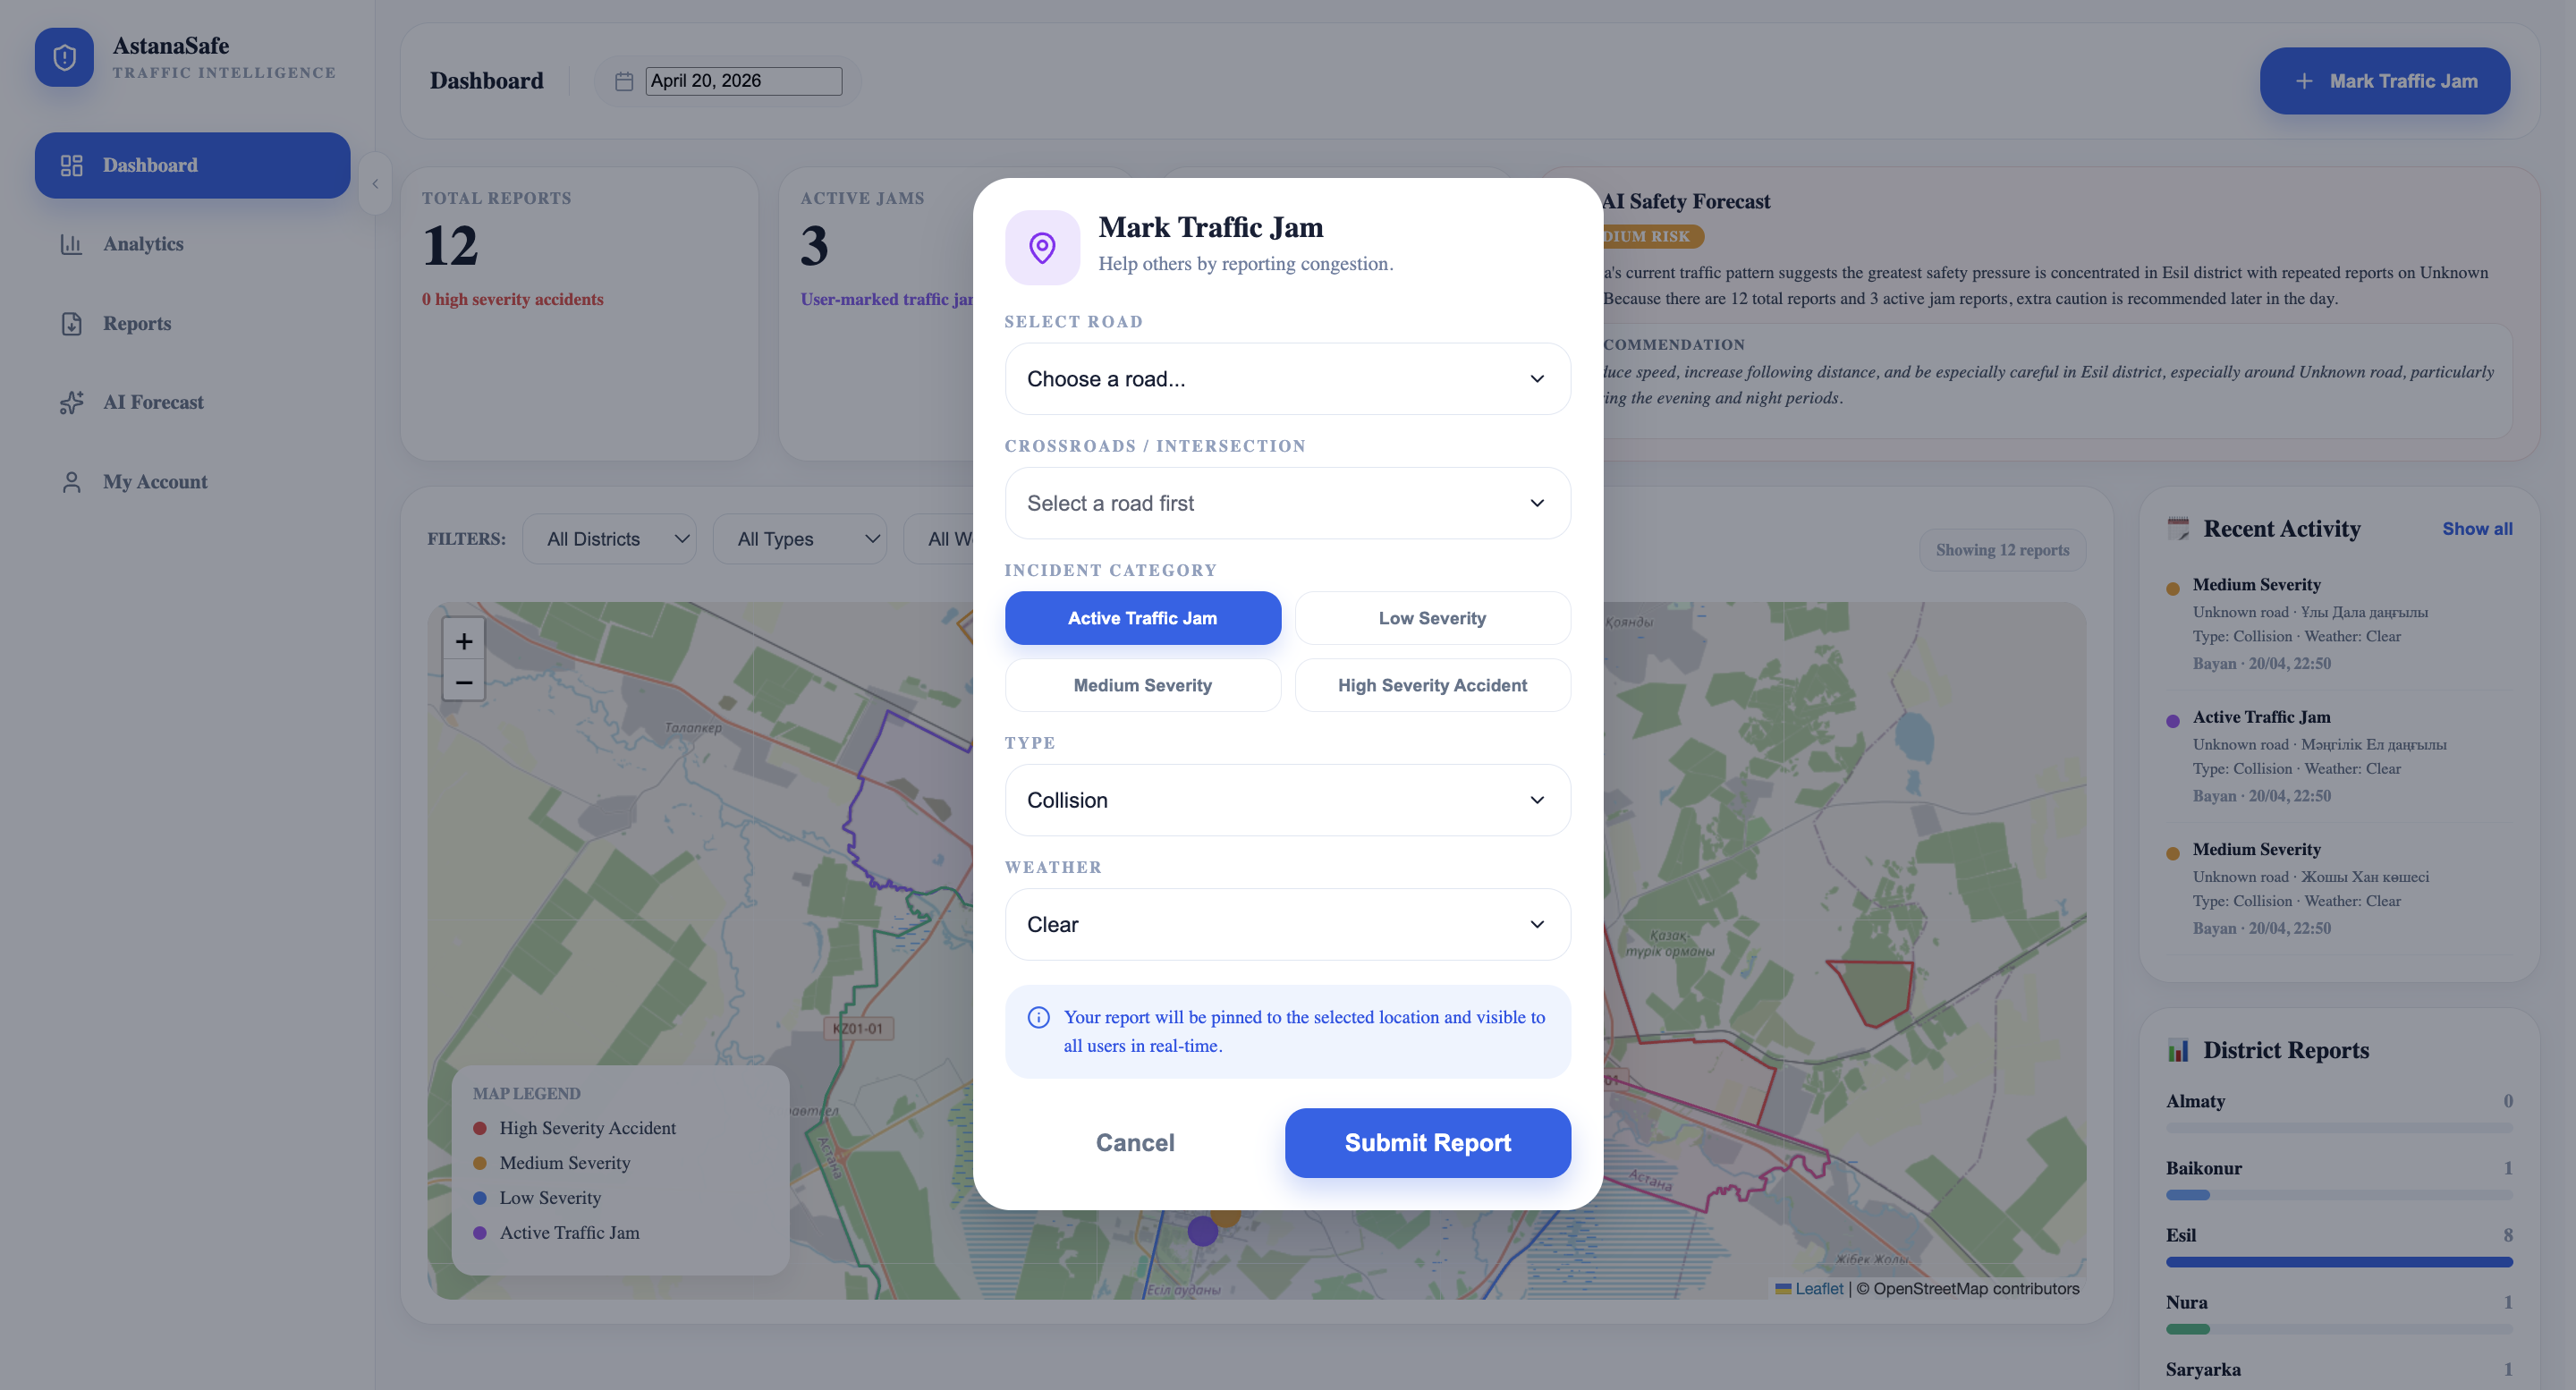
\includegraphics[width=0.72\textwidth]{sc2_mark_jam.png}
  \caption{\centering Mark Traffic Jam modal form, showing the incident category selector, type and weather dropdowns, and real-time notification message.}
  \label{fig:mark_jam}
\end{figure}

\textbf{Complete Activity Log.} Clicking "Show all" in the Recent Activity panel opens the Complete Activity Log modal. This panel displays a scrollable, searchable list of all reports for the selected date, filterable by type (All, Accident, Traffic). Summary statistics at the top of the modal show Total Logs: 12, Recent Hour: 0, Accidents: 9, Traffic Jams: 3. Each row in the log includes an icon reflecting severity, the incident category with a coloured badge, the road location, a description, and a precise timestamp. A close icon on each row allows the owner to remove their report directly from this view. Figure~\ref{fig:activity_log} presents the Complete Activity Log modal with the full list of reports for the test session.

\begin{figure}[H]
  \centering
  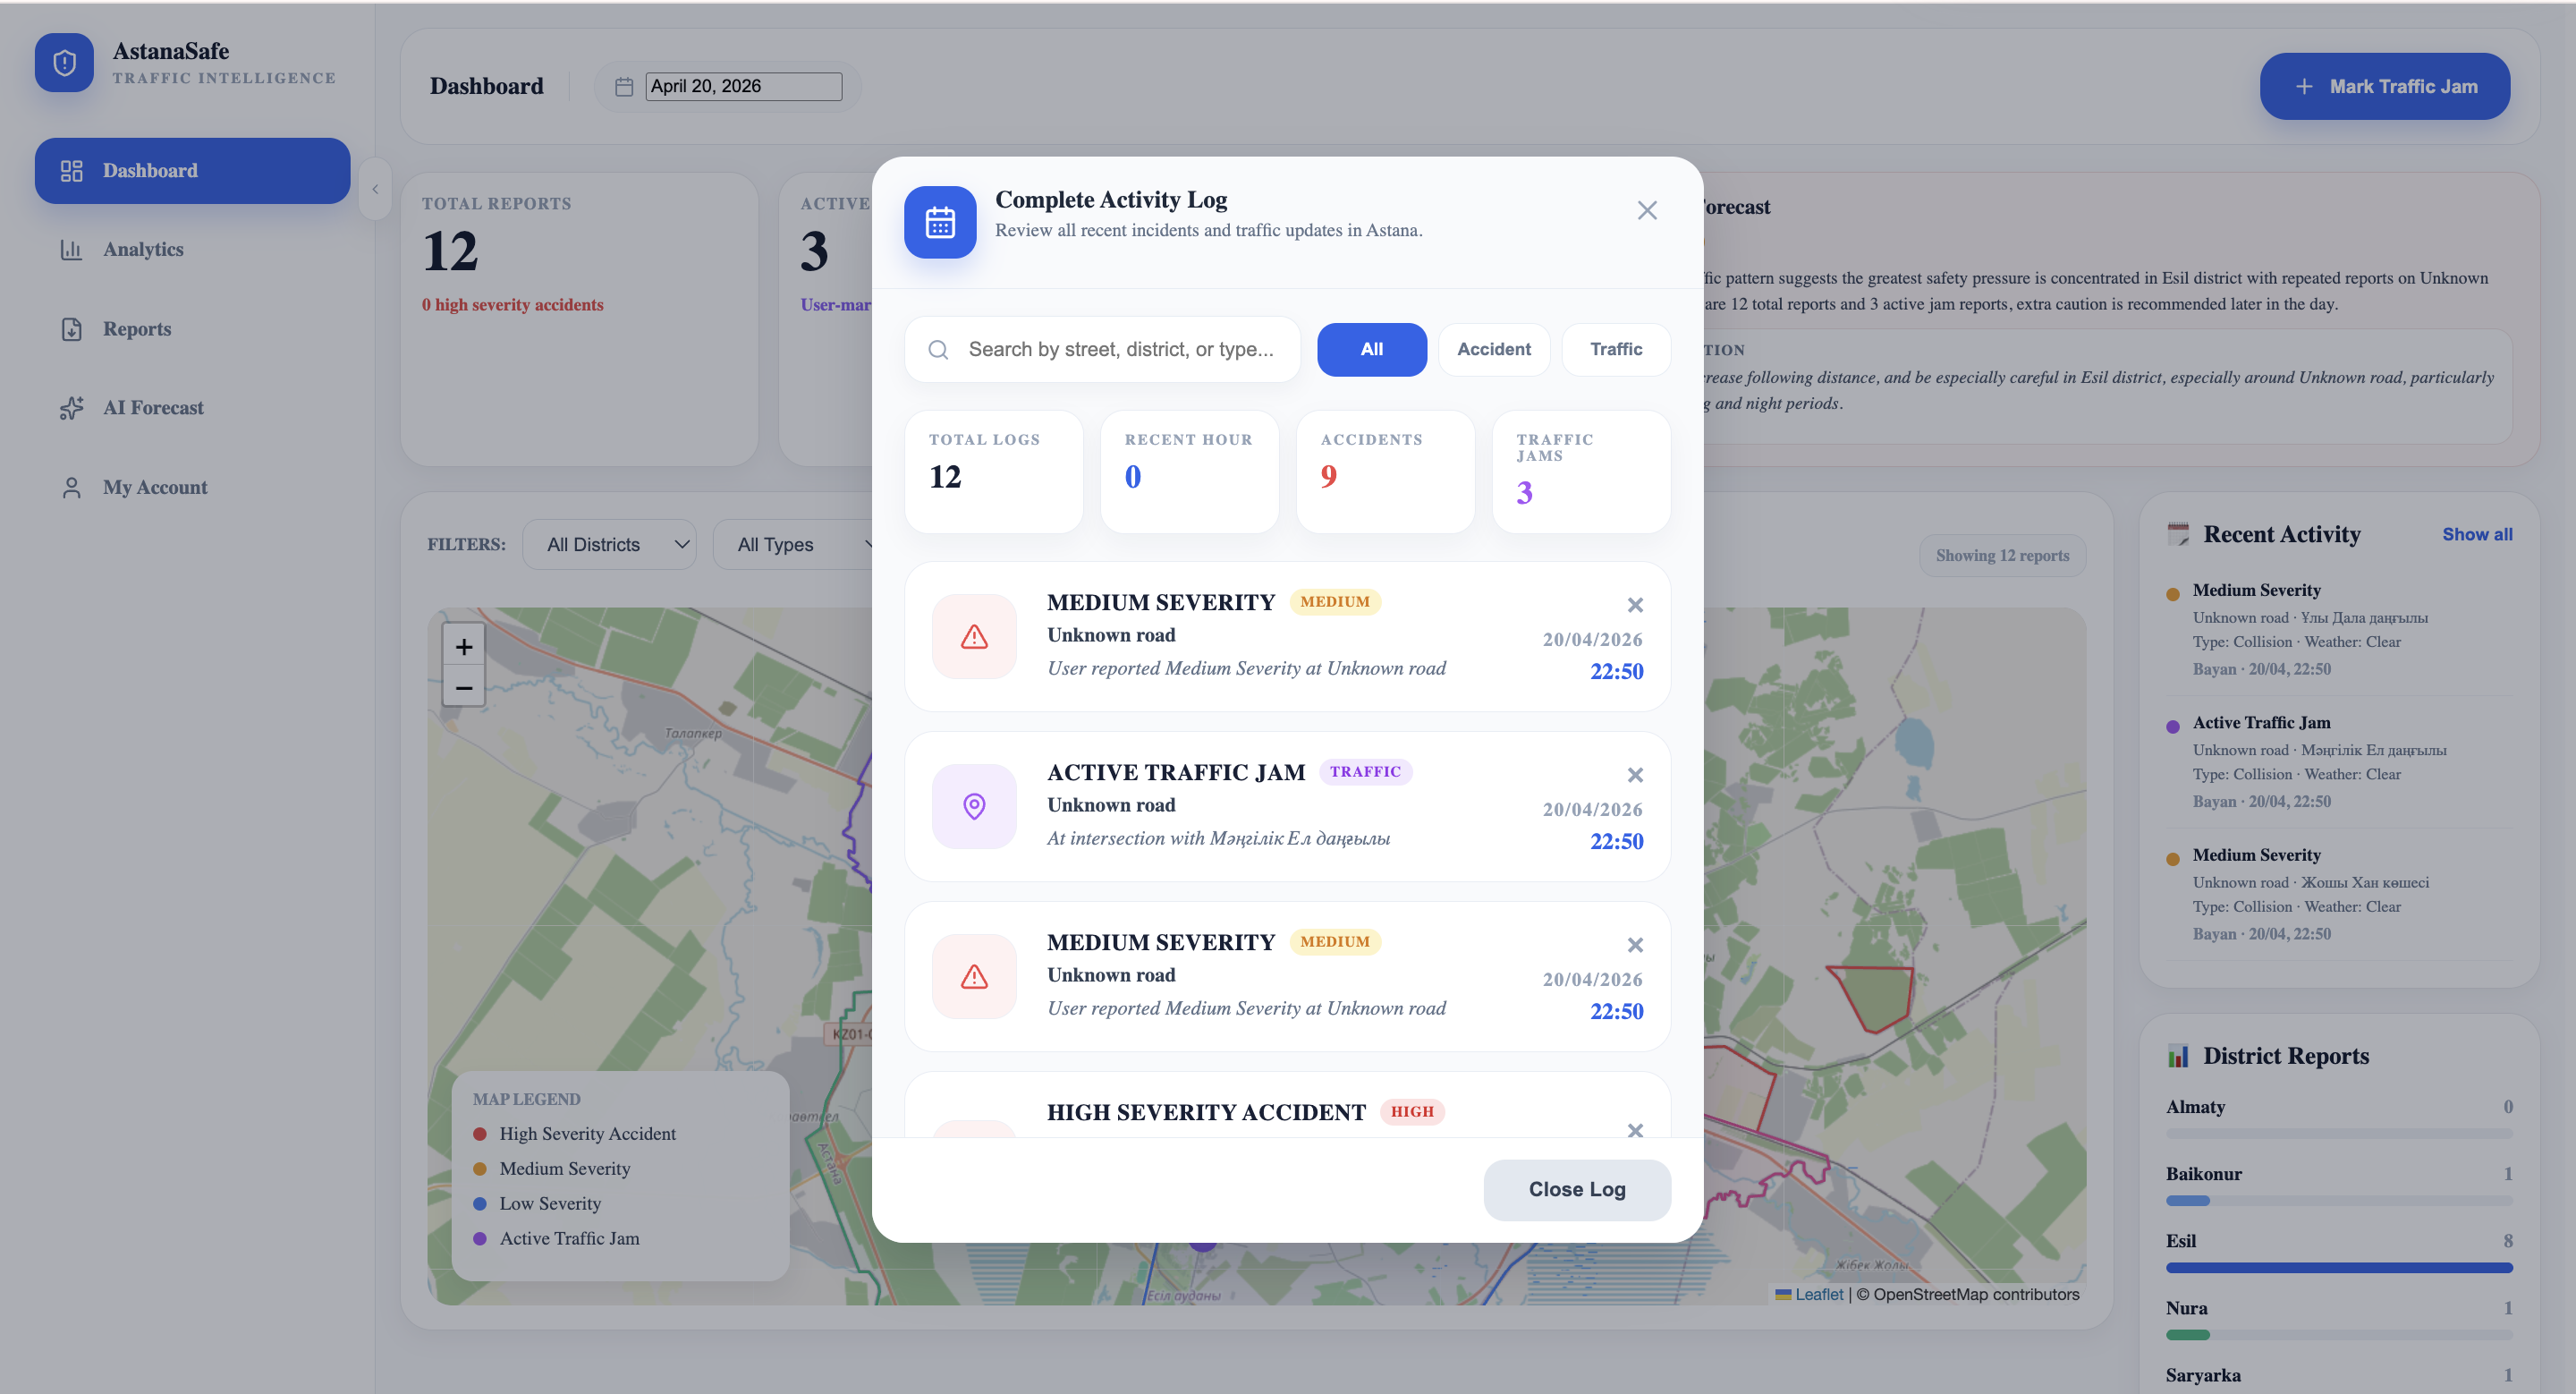
\includegraphics[width=0.72\textwidth]{sc3_activity_log.png}
  \caption{\centering Complete Activity Log modal, displaying 12 total logs including 9 accidents and 3 traffic jams, with search and filter controls.}
  \label{fig:activity_log}
\end{figure}

\textbf{Filtering system.} All pages in the system expose filtering controls appropriate to their context. On the Dashboard, three dropdown filters allow the user to restrict the visible map markers by district, incident type (collision, pedestrian, rollover, traffic jam), and weather condition (clear, rain, snow, fog). On the Analytics page, the global date picker updates all charts simultaneously. On the Reports page, a Start Date and End Date pair allows selection of an arbitrary date range, with a Clear Dates link to reset to the topbar date. On the Account page, the user can filter their personal report history by type, severity, and custom date range. These layered filtering mechanisms satisfy functional requirement FR-03 and were directly motivated by the priority given to district and time filters across all stakeholder segments in the interview study.

\subsection{Analytics Module and Advanced Analytics}

The Analytics page transforms the raw report database into a suite of visual insights designed to answer the questions identified as most important by stakeholder groups in Chapter 1: when do incidents happen, what types occur most frequently, which districts are most affected, and how do weather conditions correlate with incident rates~\cite{shu2023, miranda2024}.

\textbf{KPI metrics.} Four summary cards at the top of the page display the most important aggregate statistics for the selected date. For April 20, 2026, these values are: Total Incidents: 12 (Historical + User Reports), High Severity Ratio: 8.3\% (Combined Daily Severity), Peak Incident Hour: 12:00 (Combined Daily Activity), and Safe Districts: 4/6 (Based on all incidents). These figures provide an immediate situational overview before the user engages with the detailed charts below.

\textbf{Hourly Incident Distribution.} A blue line chart plots incident count against each hour of the 24-hour day. For the test session, a sharp peak is visible at 12:00, where the count reaches approximately 12, with all other hours at or near zero. This pattern provides direct evidence for which parts of the day require heightened attention and directly supports the temporal analysis requirements identified by transport specialists and researchers in the interview study.

\textbf{Incident Types.} A donut chart on the right side of the first chart row shows the distribution of incident types. In the test session, the chart is dominated by the collision category, illustrated in blue, indicating that vehicle-to-vehicle impacts account for the majority of reported incidents for this date.

Figure~\ref{fig:analytics} shows the Analytics page with KPI cards and the first row of charts.

\begin{figure}[H]
  \centering
  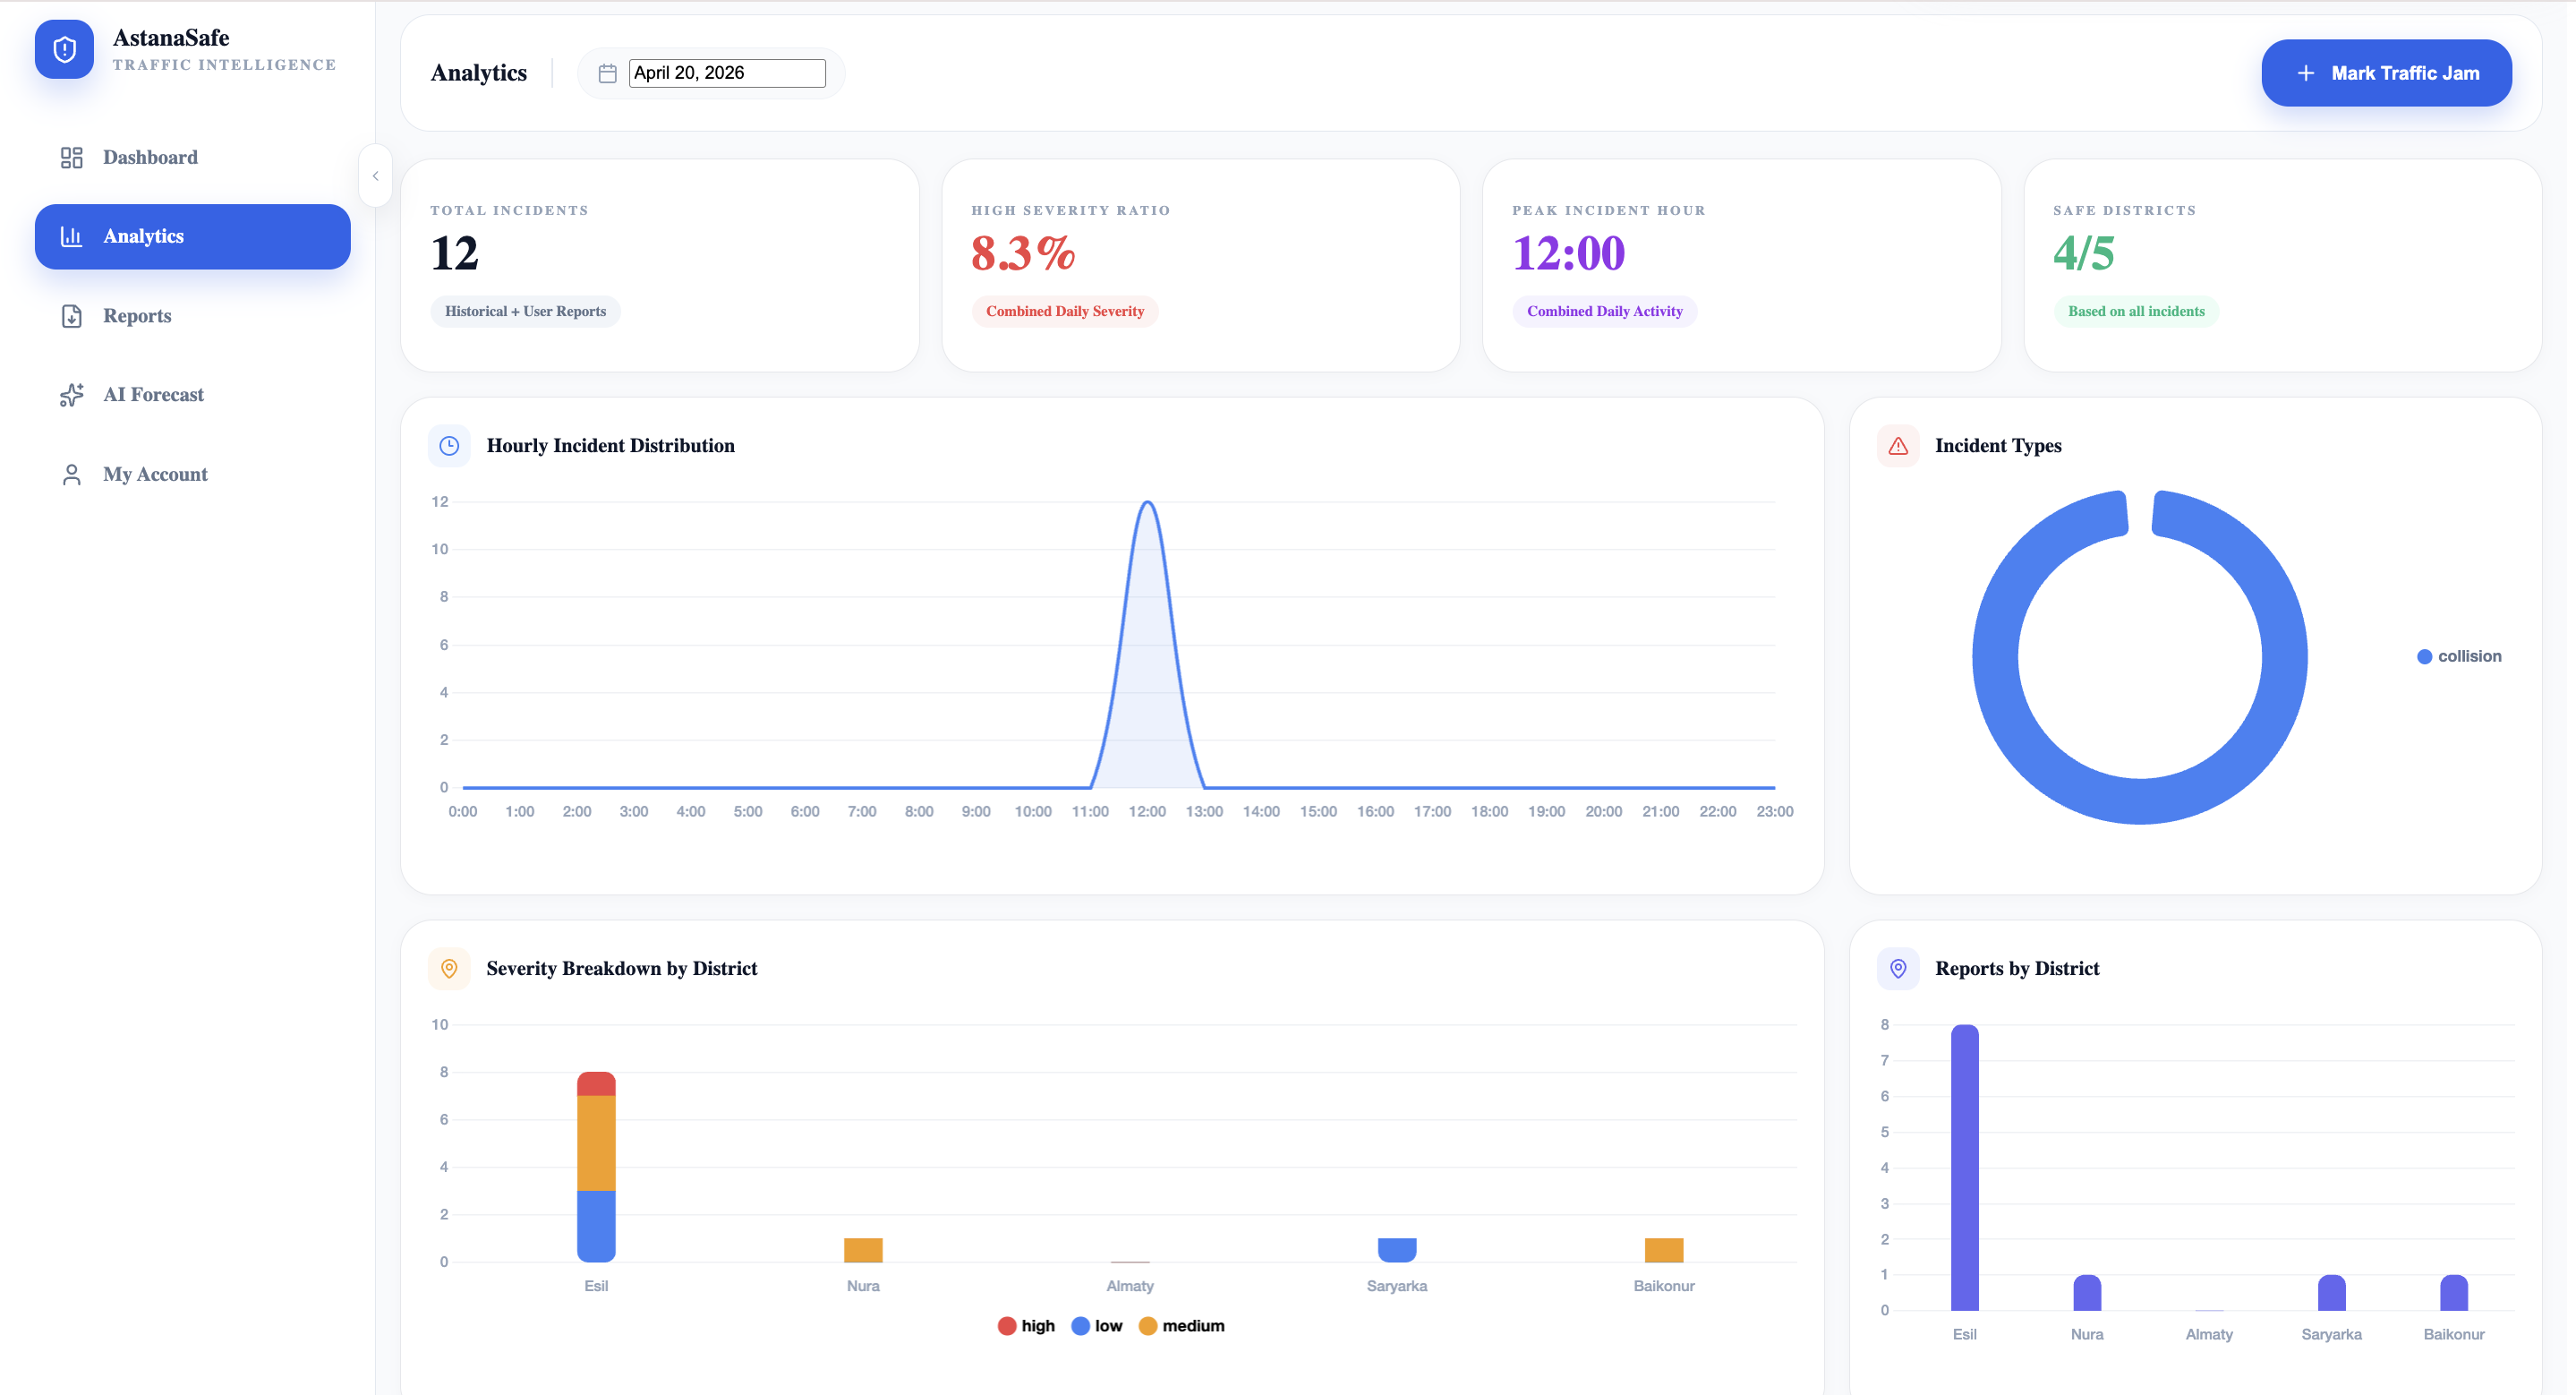
\includegraphics[width=\textwidth]{sc4_analytics.png}
  \caption{\centering Analytics page: KPI summary cards (12 total incidents, 8.3\% high severity, peak at 12:00, 4/6 safe districts), hourly incident distribution line chart, and incident types donut chart}
  \label{fig:analytics}
\end{figure}

\textbf{Severity Breakdown by District.} A stacked bar chart in the second row shows incident counts divided by severity for each of the six districts. Esil displays the tallest combined bar, composed of high, medium, and low severity segments, while Nura and Baikonur show smaller bars consisting of medium-severity incidents only, and Almaty, Saryarka, and Sarayshyq contribute minor bars. This visualisation allows an analyst to compare both the volume and the seriousness of incidents across districts in a single view.

\textbf{Reports by District.} A purple bar chart alongside the stacked severity chart shows the total report count per district without severity subdivision, confirming Esil as the most active district with 8 reports, followed by Nura and Saryarka.

\textbf{Top 8 Congested Arteries.} A horizontal bar chart in the third row ranks roads by the density of traffic jam reports submitted against them. In the test session the chart shows three entries: Unknown road with the longest bar, followed by M\k{a}ng\'{i}l\'{i}k El dan\u{g}y\l{}y and Ykshnam k\"{o}shes\'{i}. This ranking directly informs transport planners about the locations experiencing the greatest frequency of user-reported congestion, supporting the congestion monitoring objective established in Section 1.2.2.

\textbf{Weather Impact.} A bar and line combination chart on the right of the third row plots incident count against weather category. In the test session, clear weather accounts for the highest count (approximately 12 incidents), while all other categories (rain, ice, snow, fog, unknown) show zero incidents. This reflects the composition of the test dataset for this specific date and demonstrates that the weather correlation module functions correctly, attaching condition data to each record at submission time.

Figure~\ref{fig:analytics2} shows the lower portion of the Analytics page, including the severity breakdown, district report count, congested arteries chart, and weather impact chart.

\begin{figure}[H]
  \centering
  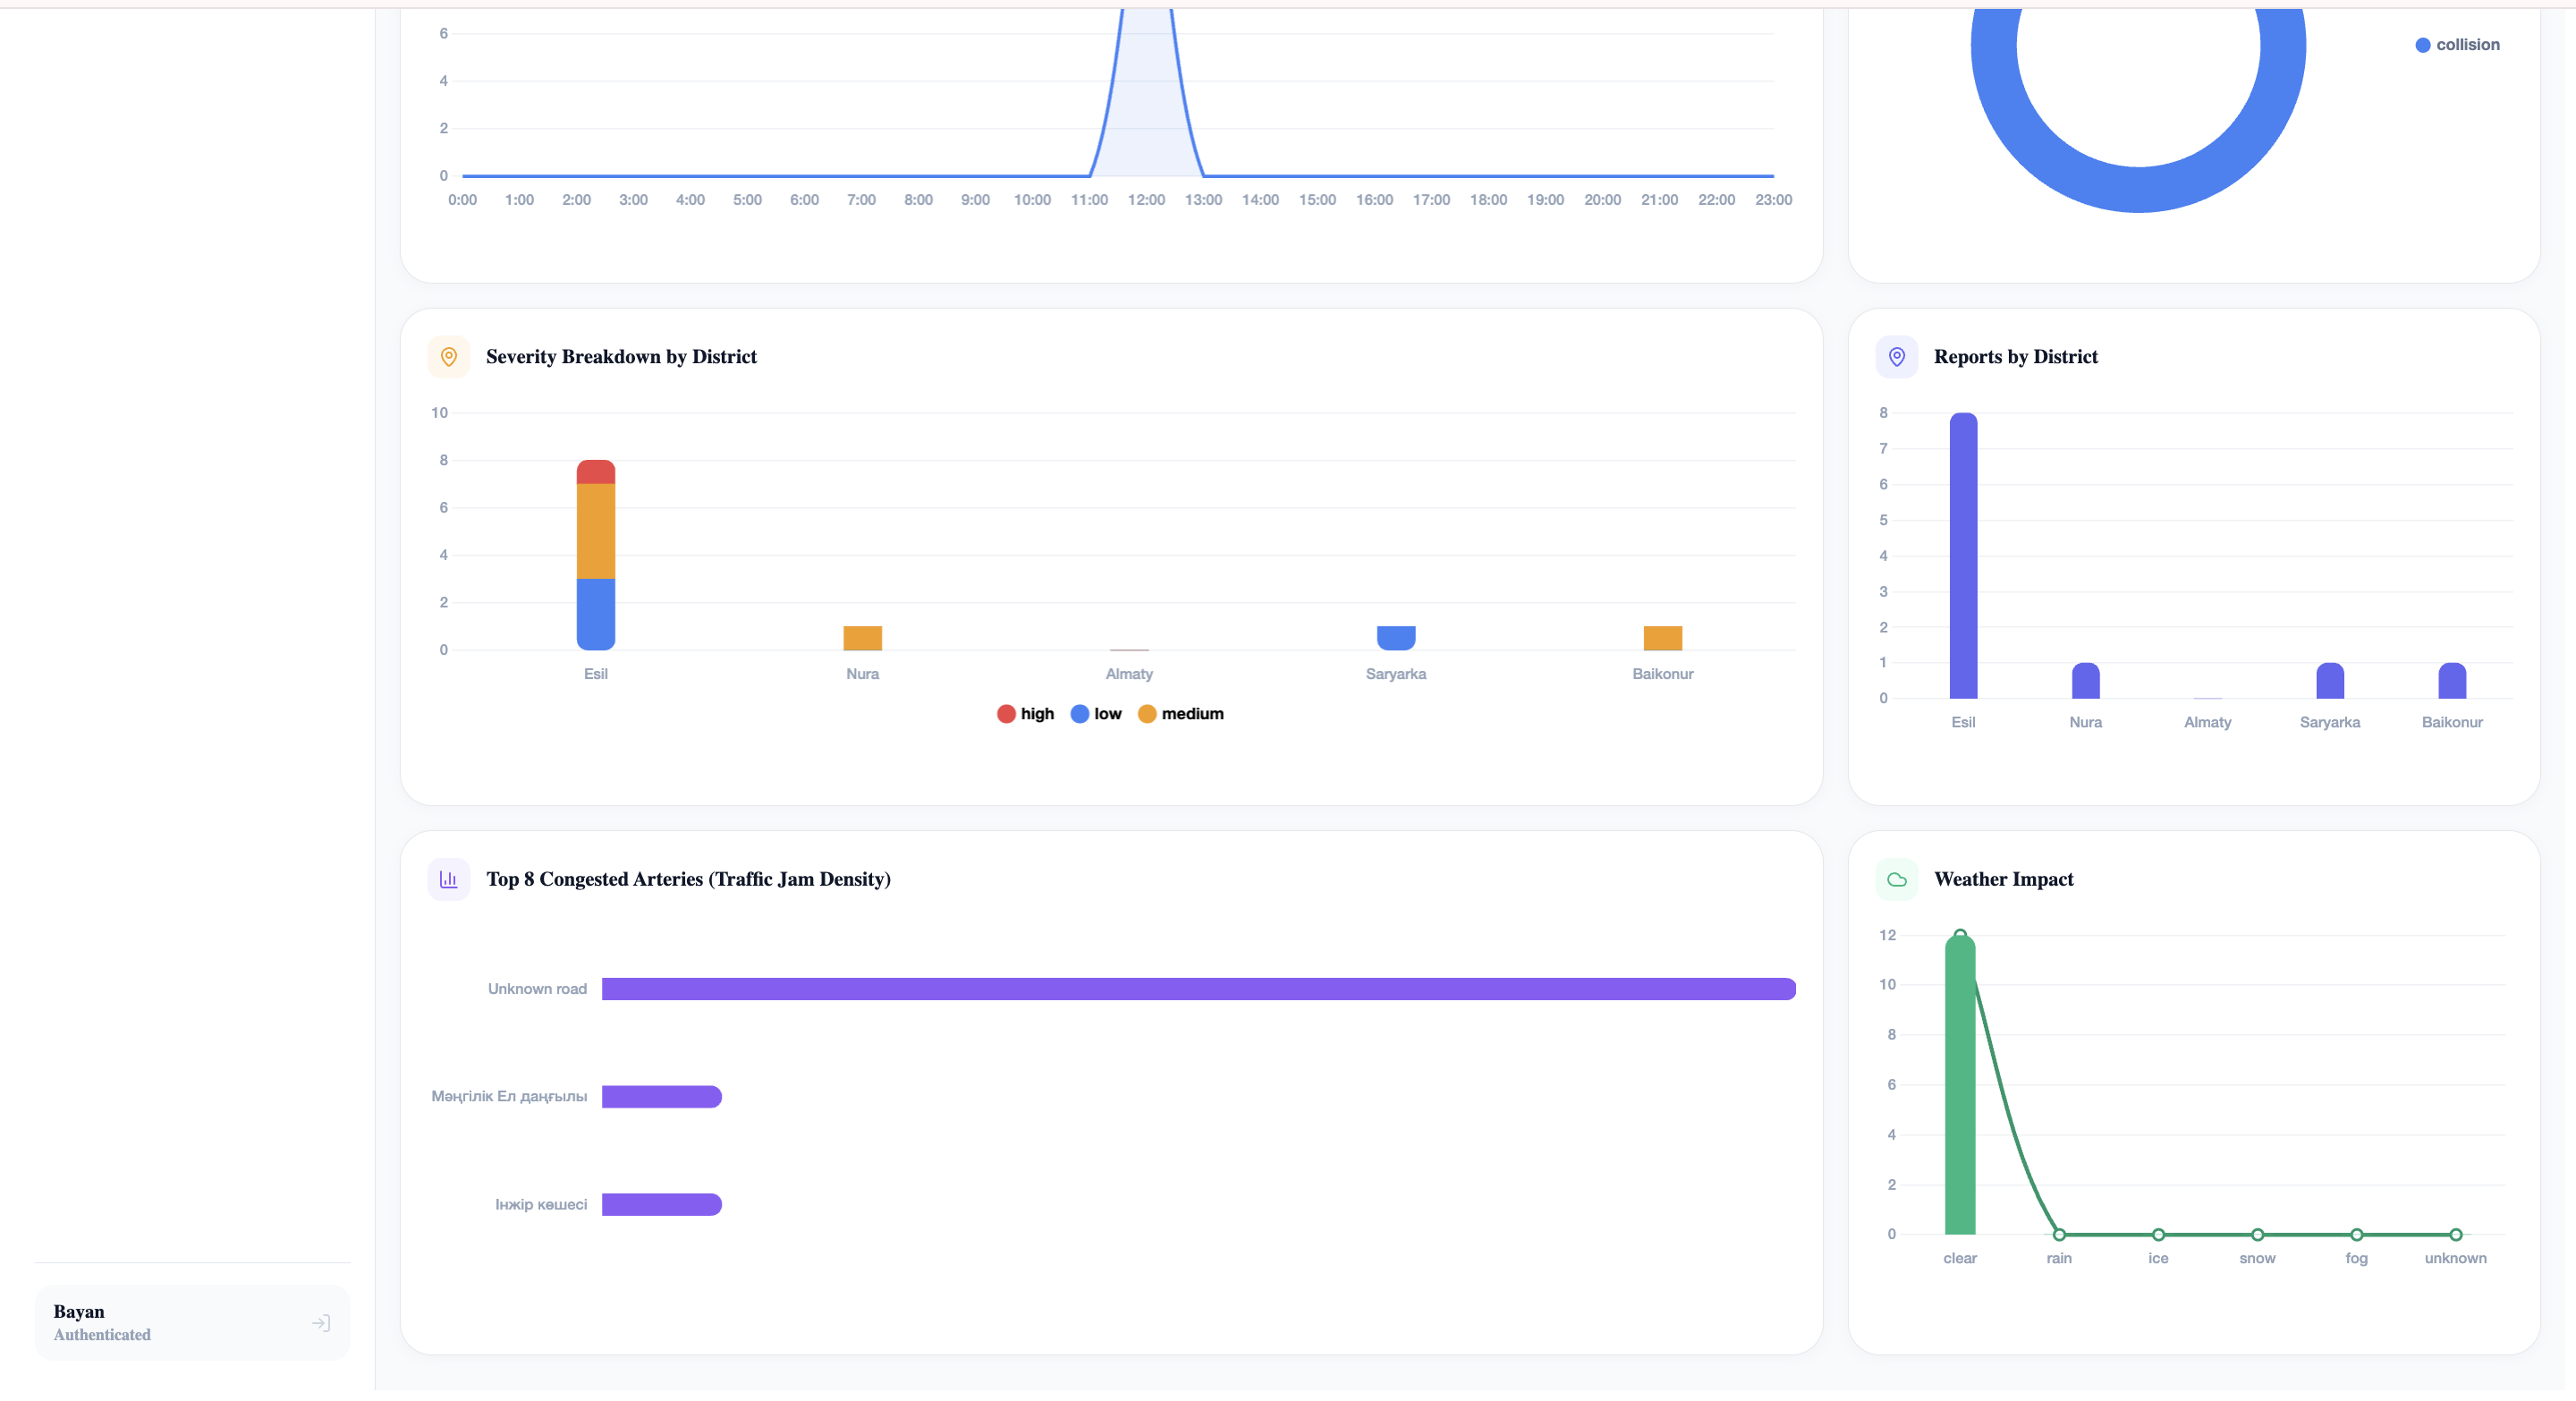
\includegraphics[width=\textwidth]{sc5_analytics2.png}
  \caption{\centering Analytics page (continued): severity breakdown by district, reports by district, top 8 congested arteries (traffic jam density), and weather impact chart.}
  \label{fig:analytics2}
\end{figure}

The analytics module directly addresses the advanced analysis requirements described in the project specification: the weather impact chart enables examination of how meteorological conditions relate to incident frequency; the congested arteries chart quantifies traffic jam density per road; the hourly distribution chart supports analysis by time of day; and the severity-by-district breakdown enables district-level comparison. Together, these charts constitute the core analytical value proposition of the dashboard relative to the navigation platforms reviewed in Section 1.3.2~\cite{guo2024}.

\subsection{Reports Module}

The Reports page provides an audit trail of all recorded incidents in a structured, filterable table format. Three KPI cards at the top summarise the current filter context: Total Filtered Reports: 12 (Historical + user data), High Severity Rate: 8\%, and Most Active District: Esil. The main content area is titled "Historical Safety Data" with the subtitle "Audit trail of historical accidents and live user reports in Astana."

Above the data table, a date range filter panel with Start Date and End Date fields enables the user to select an arbitrary historical window. Two export buttons - CSV and PDF Export - allow records matching the current filter to be downloaded in the respective format, satisfying FR-06 and the data export requirements cited by research and student users during the interviews.

The table itself contains seven columns: Date and Time, District, Type (displayed as a rounded badge), Severity (displayed with a coloured dot and text label), Weather, and Actions. The Actions column provides an arrow button that navigates the user to the Dashboard page and highlights the corresponding map marker for the selected record, creating a direct visual link between the tabular archive and the spatial representation. For the test session, eight records are visible on the page, all dated 20.04.2026, spanning Esil and Nura districts, with types including Collision, Traffic Jam, and Other, and severities ranging from LOW to HIGH. Figure~\ref{fig:reports} shows the Reports page with the populated data table.

\begin{figure}[H]
  \centering
  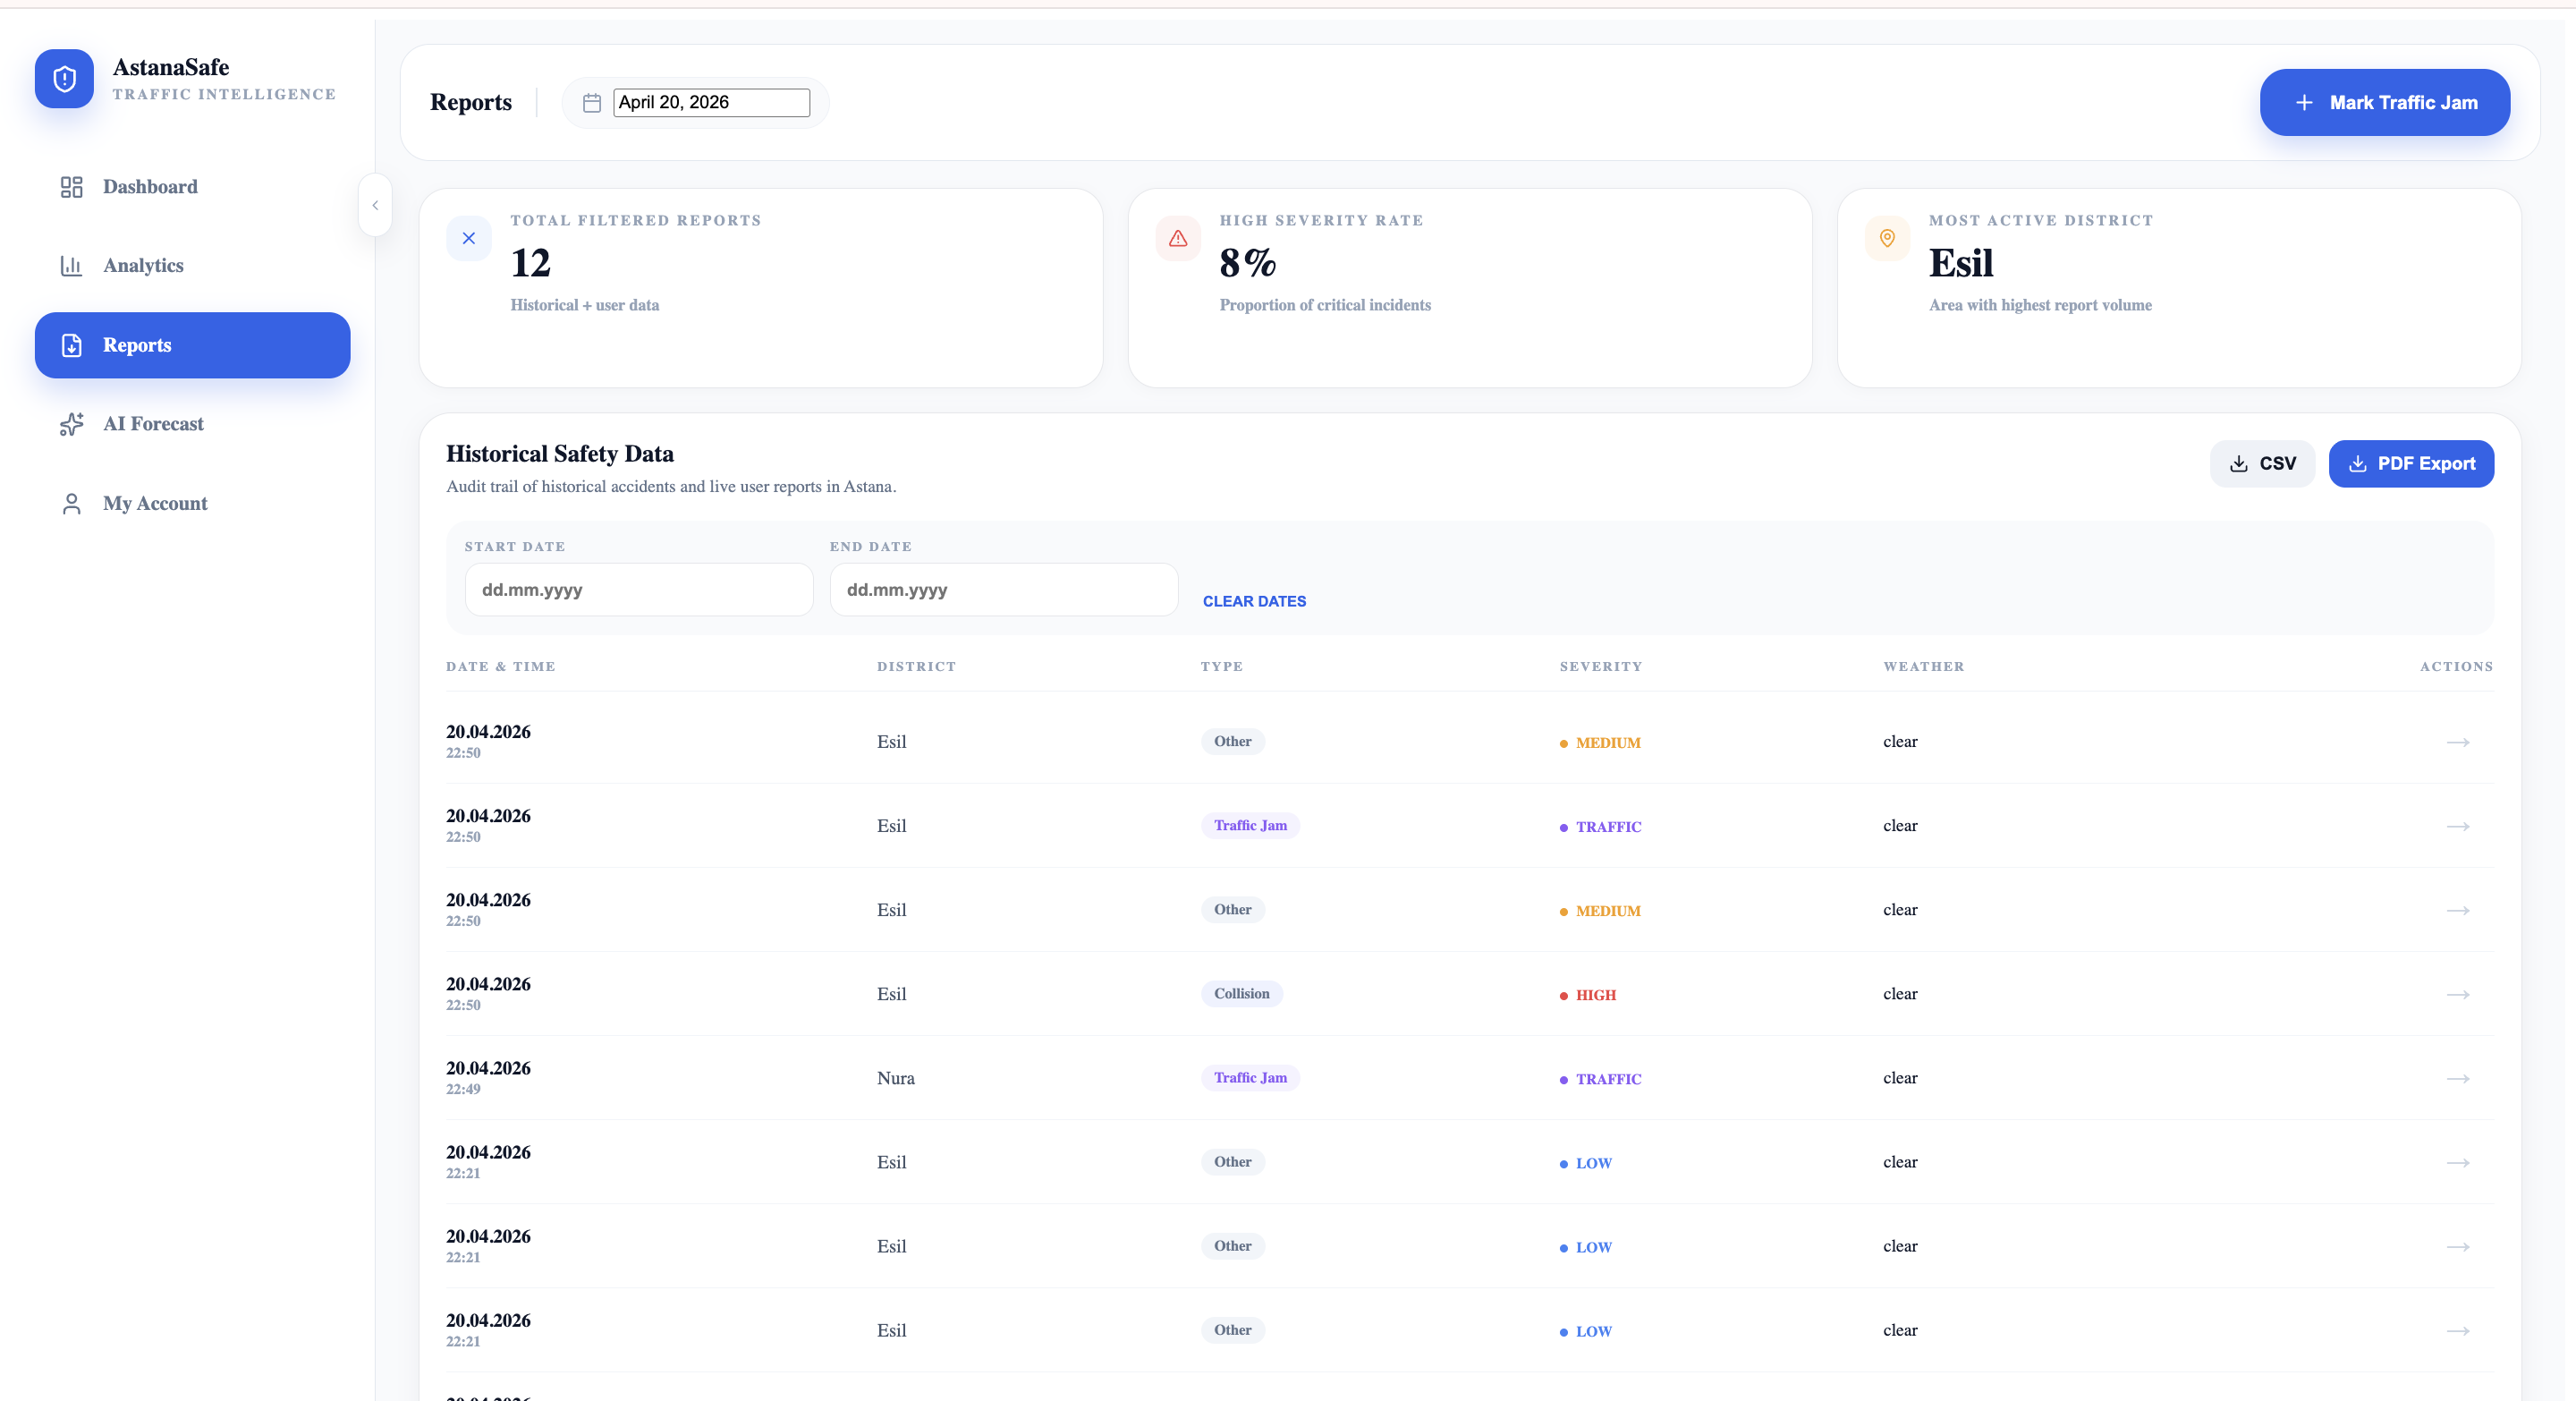
\includegraphics[width=\textwidth]{sc6_reports.png}
  \caption{\centering Reports page: KPI cards (12 total reports, 8\% high severity rate, Esil as most active district) and Historical Safety Data table with date filter and export controls}
  \label{fig:reports}
\end{figure}

\subsection{AI Safety Forecast Module}

The AI Forecast page provides forward-looking safety estimates derived from the current report dataset. The module uses a rule-based natural language generation approach rather than a trained machine learning model: it evaluates the total report count, the distribution of reports across districts, the count of active traffic jams, the dominant weather condition, and the hourly activity pattern, and produces structured textual assessments that are rendered in the interface as a premium gradient card~\cite{yin2021}.

The main panel displays an executive summary sentence explaining which district is under greatest pressure and why caution is recommended. For the test session dated April 20, 2026, the summary states that the greatest safety pressure is concentrated in Esil district, that there are 12 total reports and 3 active jam reports, and that extra caution is recommended later in the day.

Below the summary, four semi-transparent cards divide the risk assessment by time of day. Morning is rated LOW RISK, with the advice that conditions are expected to remain manageable though users in Esil should stay attentive. Afternoon is rated MEDIUM RISK, noting that pressure may build near Esil particularly as clear conditions continue to affect traffic flow. Evening is rated HIGH RISK, as it coincides with the strongest concentration of reports. Night is also rated HIGH RISK, reflecting reduced visibility and the persistence of active jams on the network.

The Predicted Danger Zones card identifies Esil and Baikonur as WATCH ZONE districts for the next 12 hours, with short descriptions of why each district is flagged. The AI Analysis panel on the right displays the overall risk level as MEDIUM and provides a REASONING paragraph that transparently explains the forecast basis: Esil is the busiest district, the most common type is collision, the weather is mostly clear, and there are 3 active jam reports in the backend. A Safety Recommendation panel in dark navy at the bottom advises drivers to reduce speed, increase following distance, and be especially careful in Esil district during evening and night periods. Figure~\ref{fig:forecast} shows the complete AI Forecast page.

\begin{figure}[H]
  \centering
  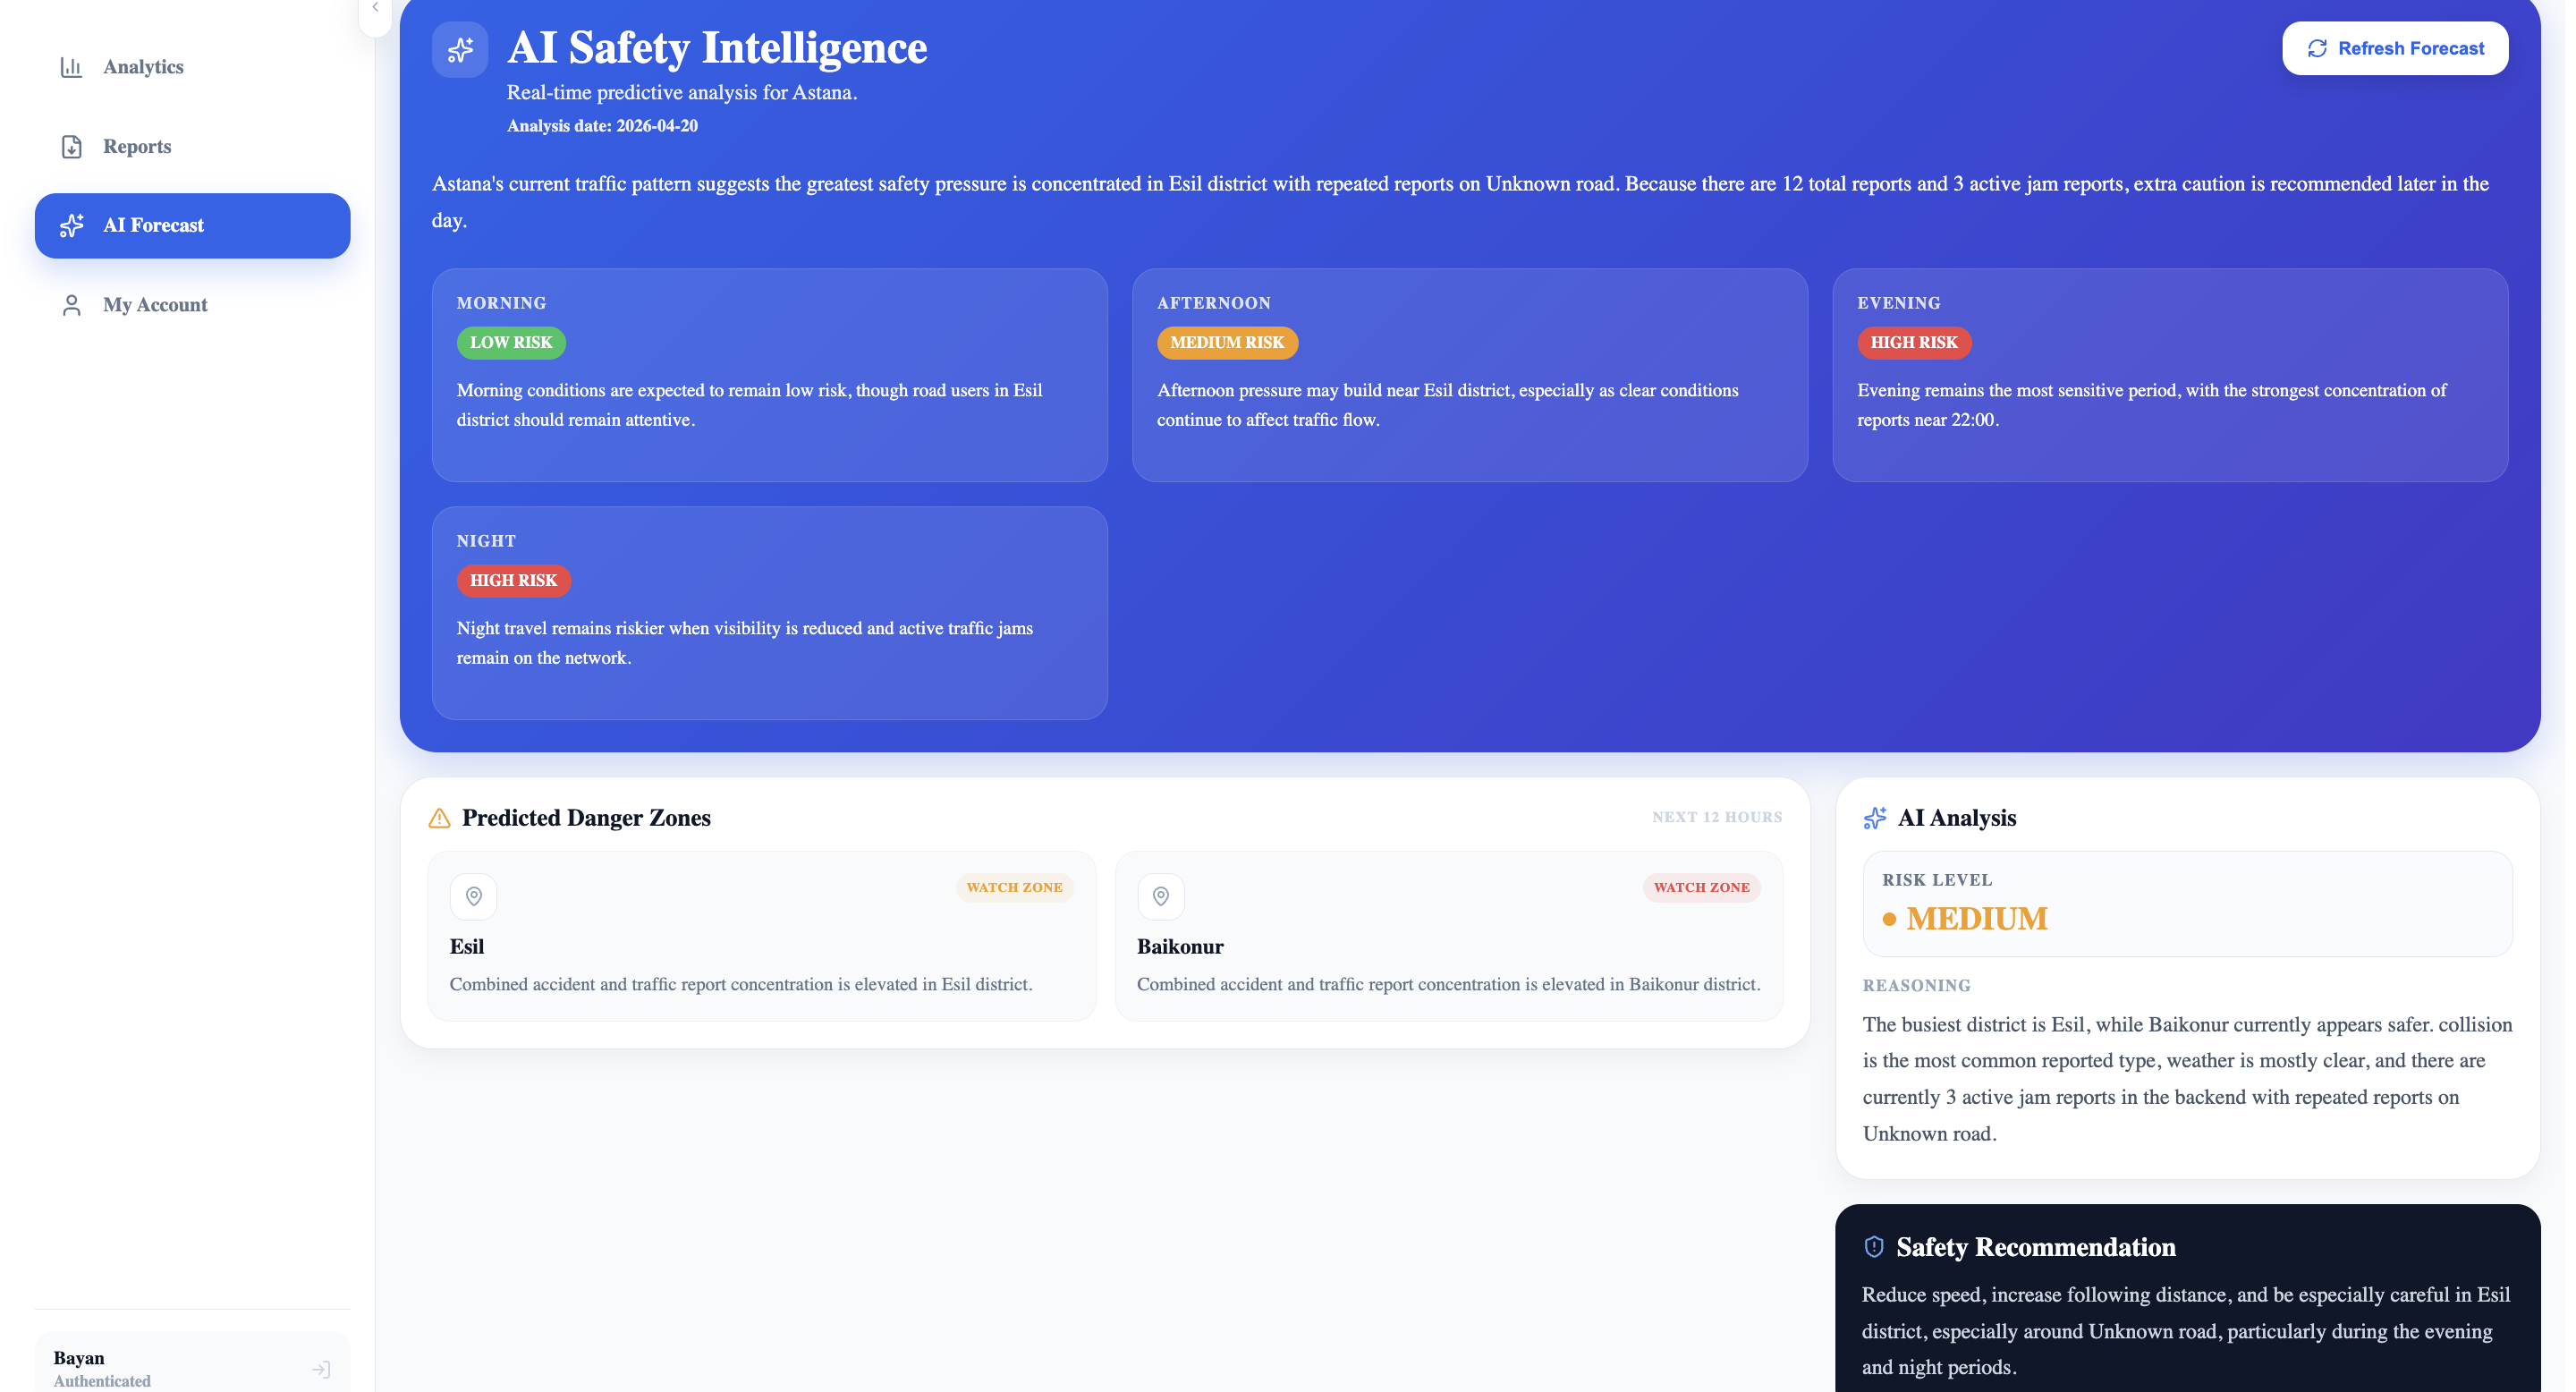
\includegraphics[width=\textwidth]{sc7_forecast.png}
  \caption{\centering AI Forecast page: time-of-day risk cards, predicted danger zones, AI analysis panel with MEDIUM overall risk, and safety recommendation.}
  \label{fig:forecast}
\end{figure}

\subsection{Account and Settings Module}

The Account page allows authenticated users to manage their identity, review their contribution history, and control their personal data. The profile summary card at the top of the page displays the user's avatar placeholder, name, contact number, and two contribution badges: 19 Total Reports and Active Contributor. Two action buttons in the upper right open the Settings modal and initiate a sign-out.

The My Recent Marks section below the profile card presents the user's submitted reports in a chronological list grouped by date. Each row shows the road name, the intersecting street, the date, a coloured severity badge, and a trash icon for deletion. Filter controls above the list allow filtering by type, severity, and custom date range. This section gives users direct management over the data they have contributed and satisfies the personal data control requirement identified in the privacy-related interview questions. Figure~\ref{fig:account} shows the Account page for the active test user.

\begin{figure}[H]
  \centering
  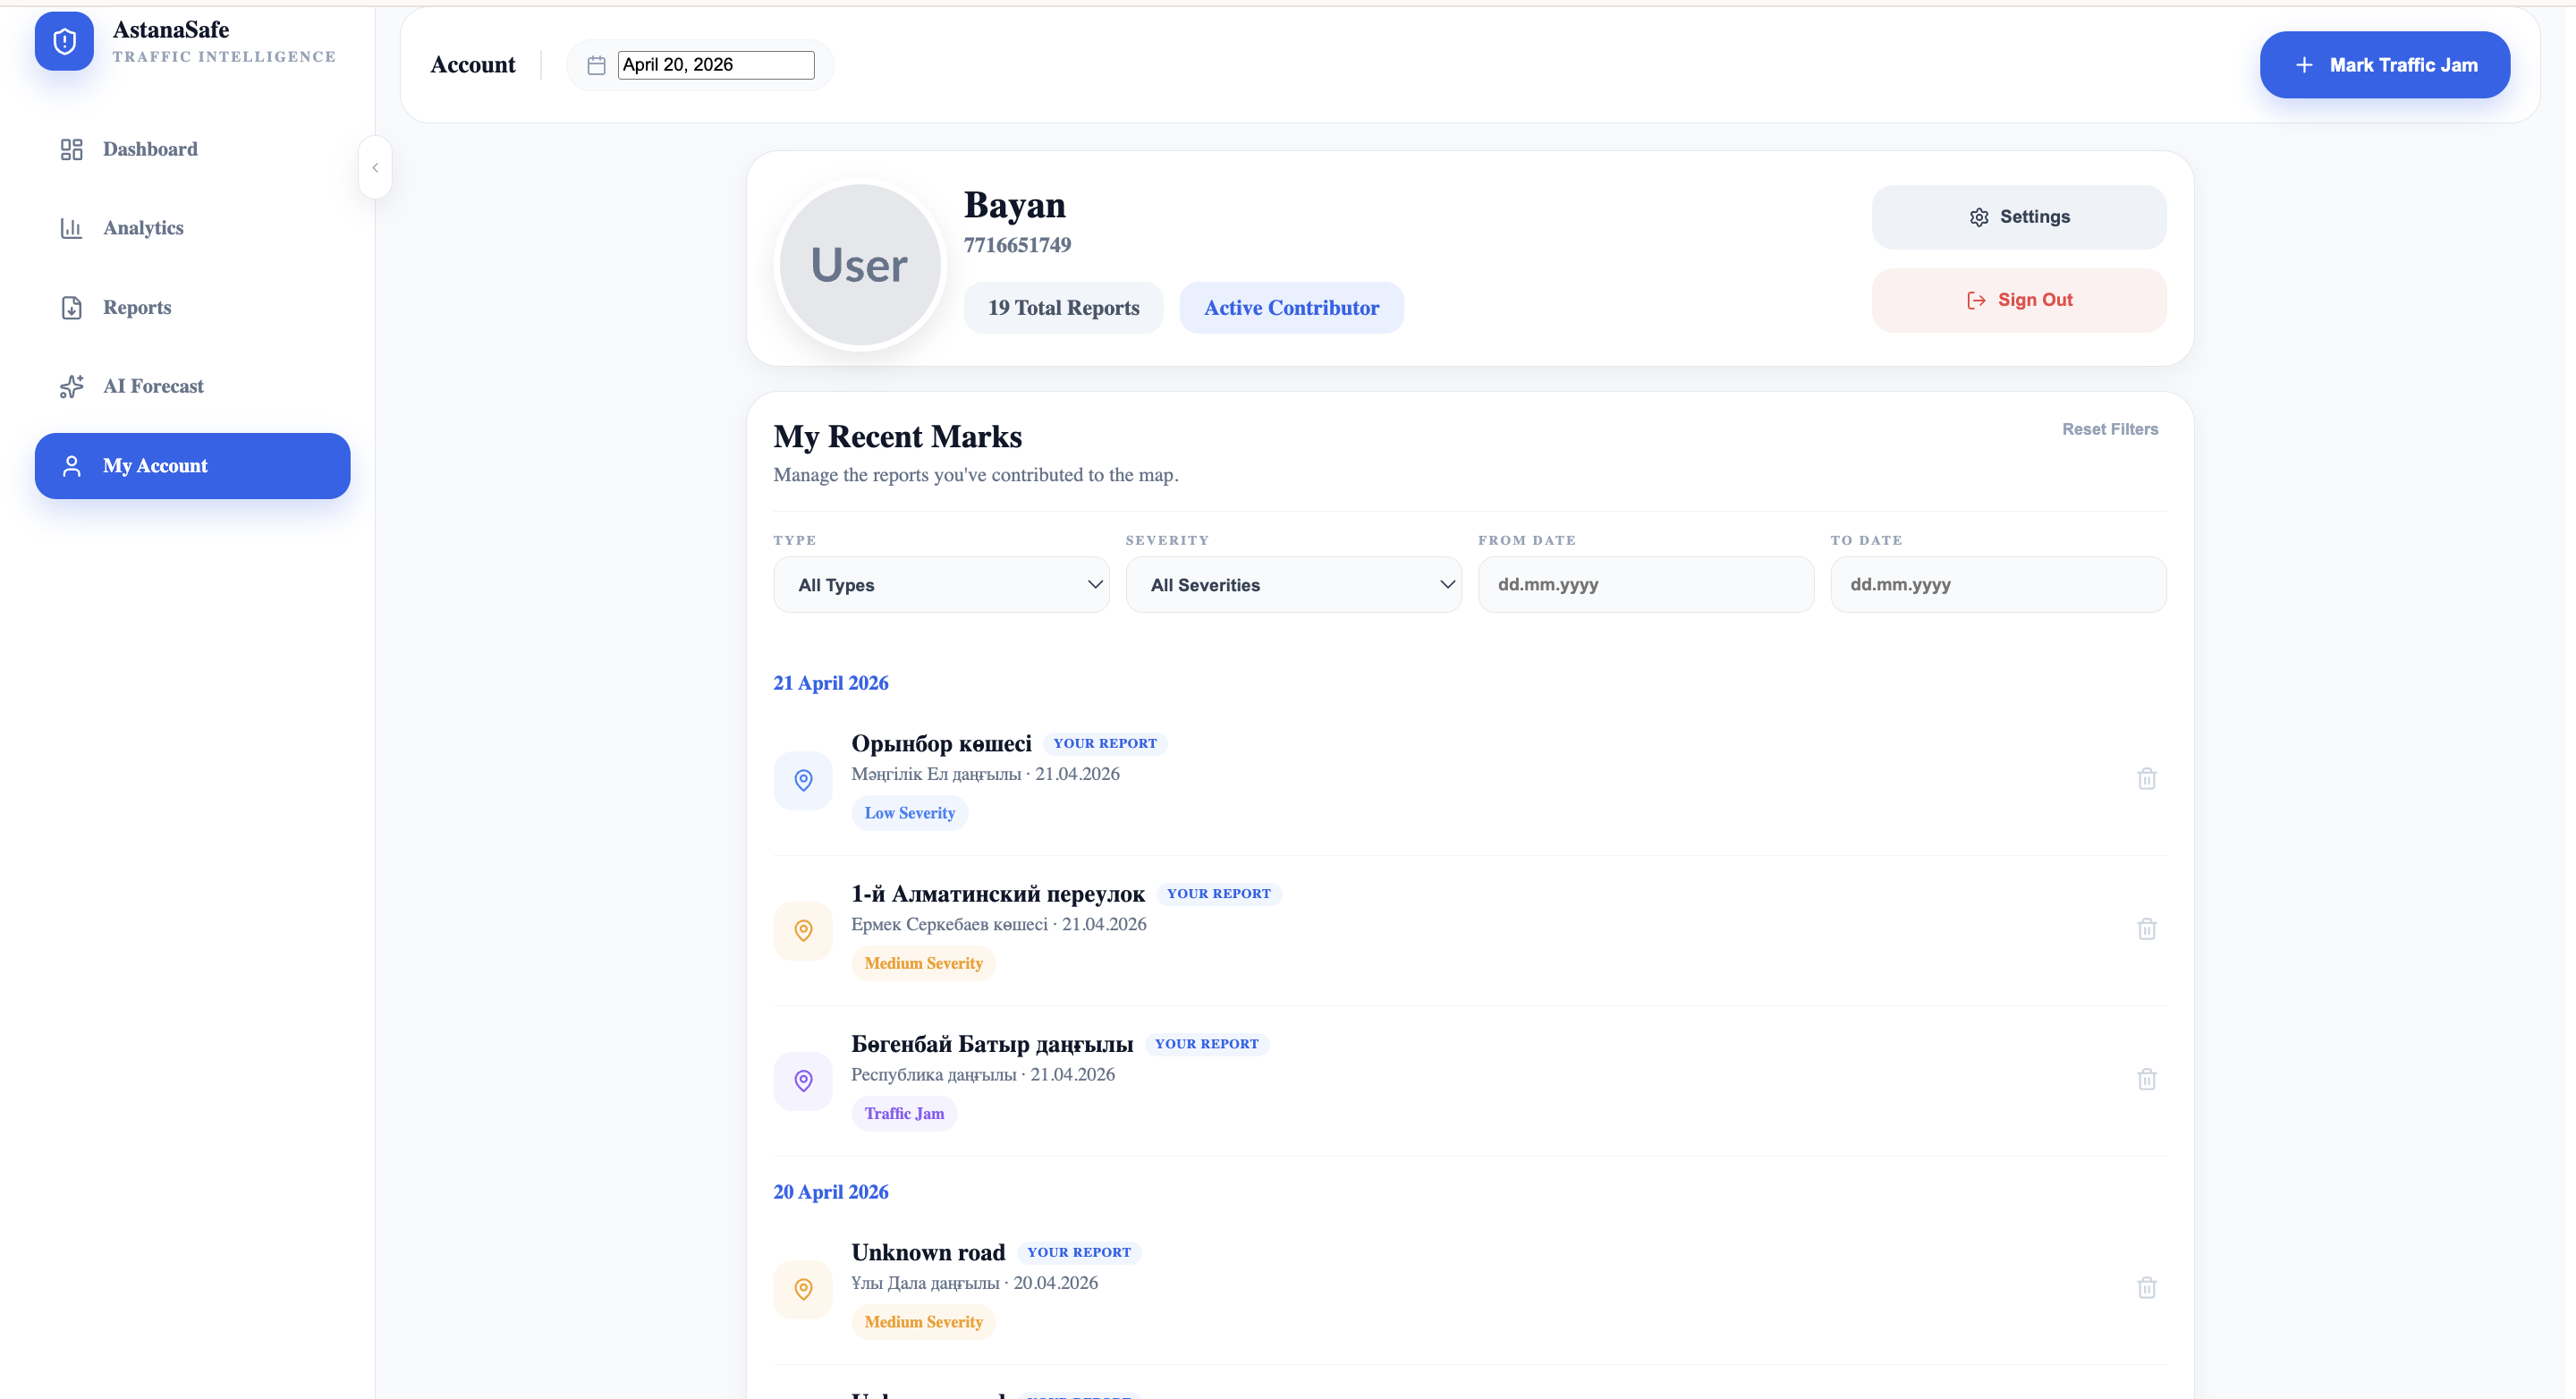
\includegraphics[width=\textwidth]{sc8_account.png}
  \caption{\centering Account page: user profile card, My Recent Marks list with severity badges, and filter controls.}
  \label{fig:account}
\end{figure}

The Settings modal is accessible from the Account page and is divided into two tabs: Profile and Privacy \& Data. The Profile tab allows the user to edit their display name and contact number, and to change their password through a three-field form (current password, new password, confirm new password). A Save Profile button commits changes to the backend. Figure~\ref{fig:settings_profile} shows the Profile tab of the Settings modal.

\begin{figure}[H]
  \centering
  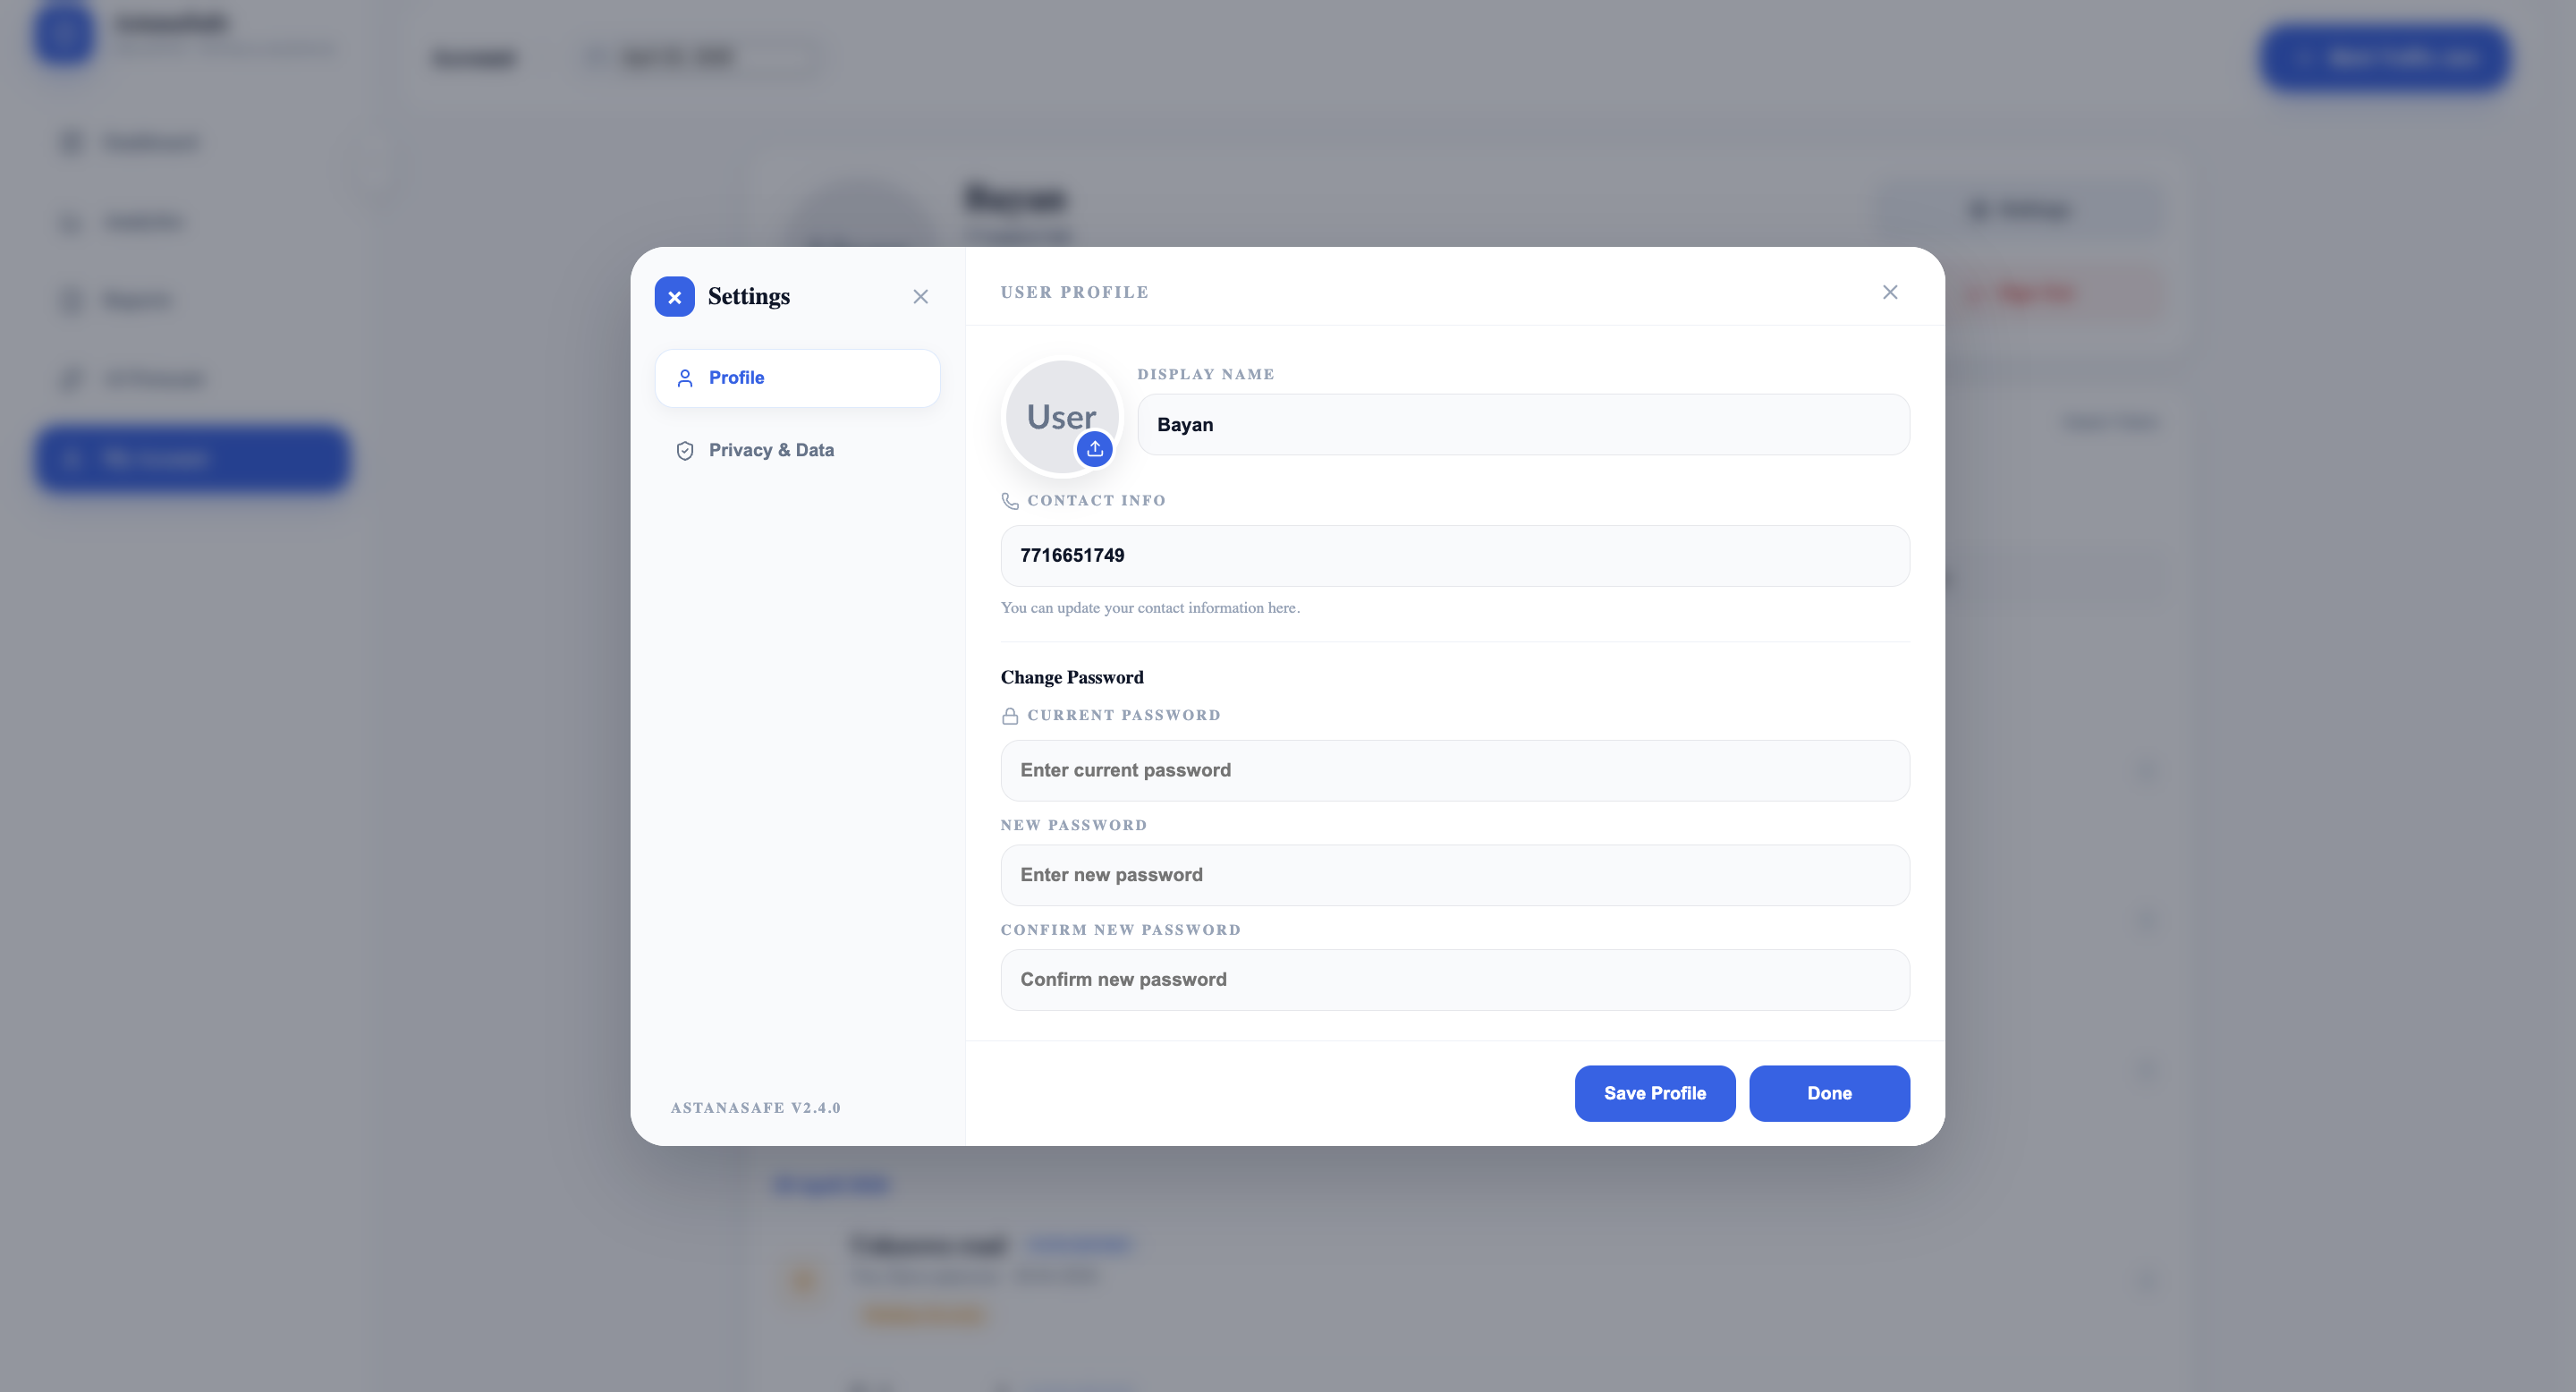
\includegraphics[width=0.75\textwidth]{sc9_settings_profile.png}
  \caption{\centering Settings modal - Profile tab: display name editor, contact information field, and change password form for the authenticated user.}
  \label{fig:settings_profile}
\end{figure}

The Privacy \& Data tab provides three data management options: an Anonymous Reporting toggle that hides the submitting user's name from public markers when enabled; a Data Management section with buttons to export the user's markers as a JSON file and to clear locally cached data; and a Danger Zone section containing a red button to permanently delete the user's account and all associated data. The application version is displayed in the lower left of both settings tabs as ASTANASAFE V2.4.0. Figure~\ref{fig:settings_privacy} shows the Privacy \& Data tab.

\begin{figure}[H]
  \centering
  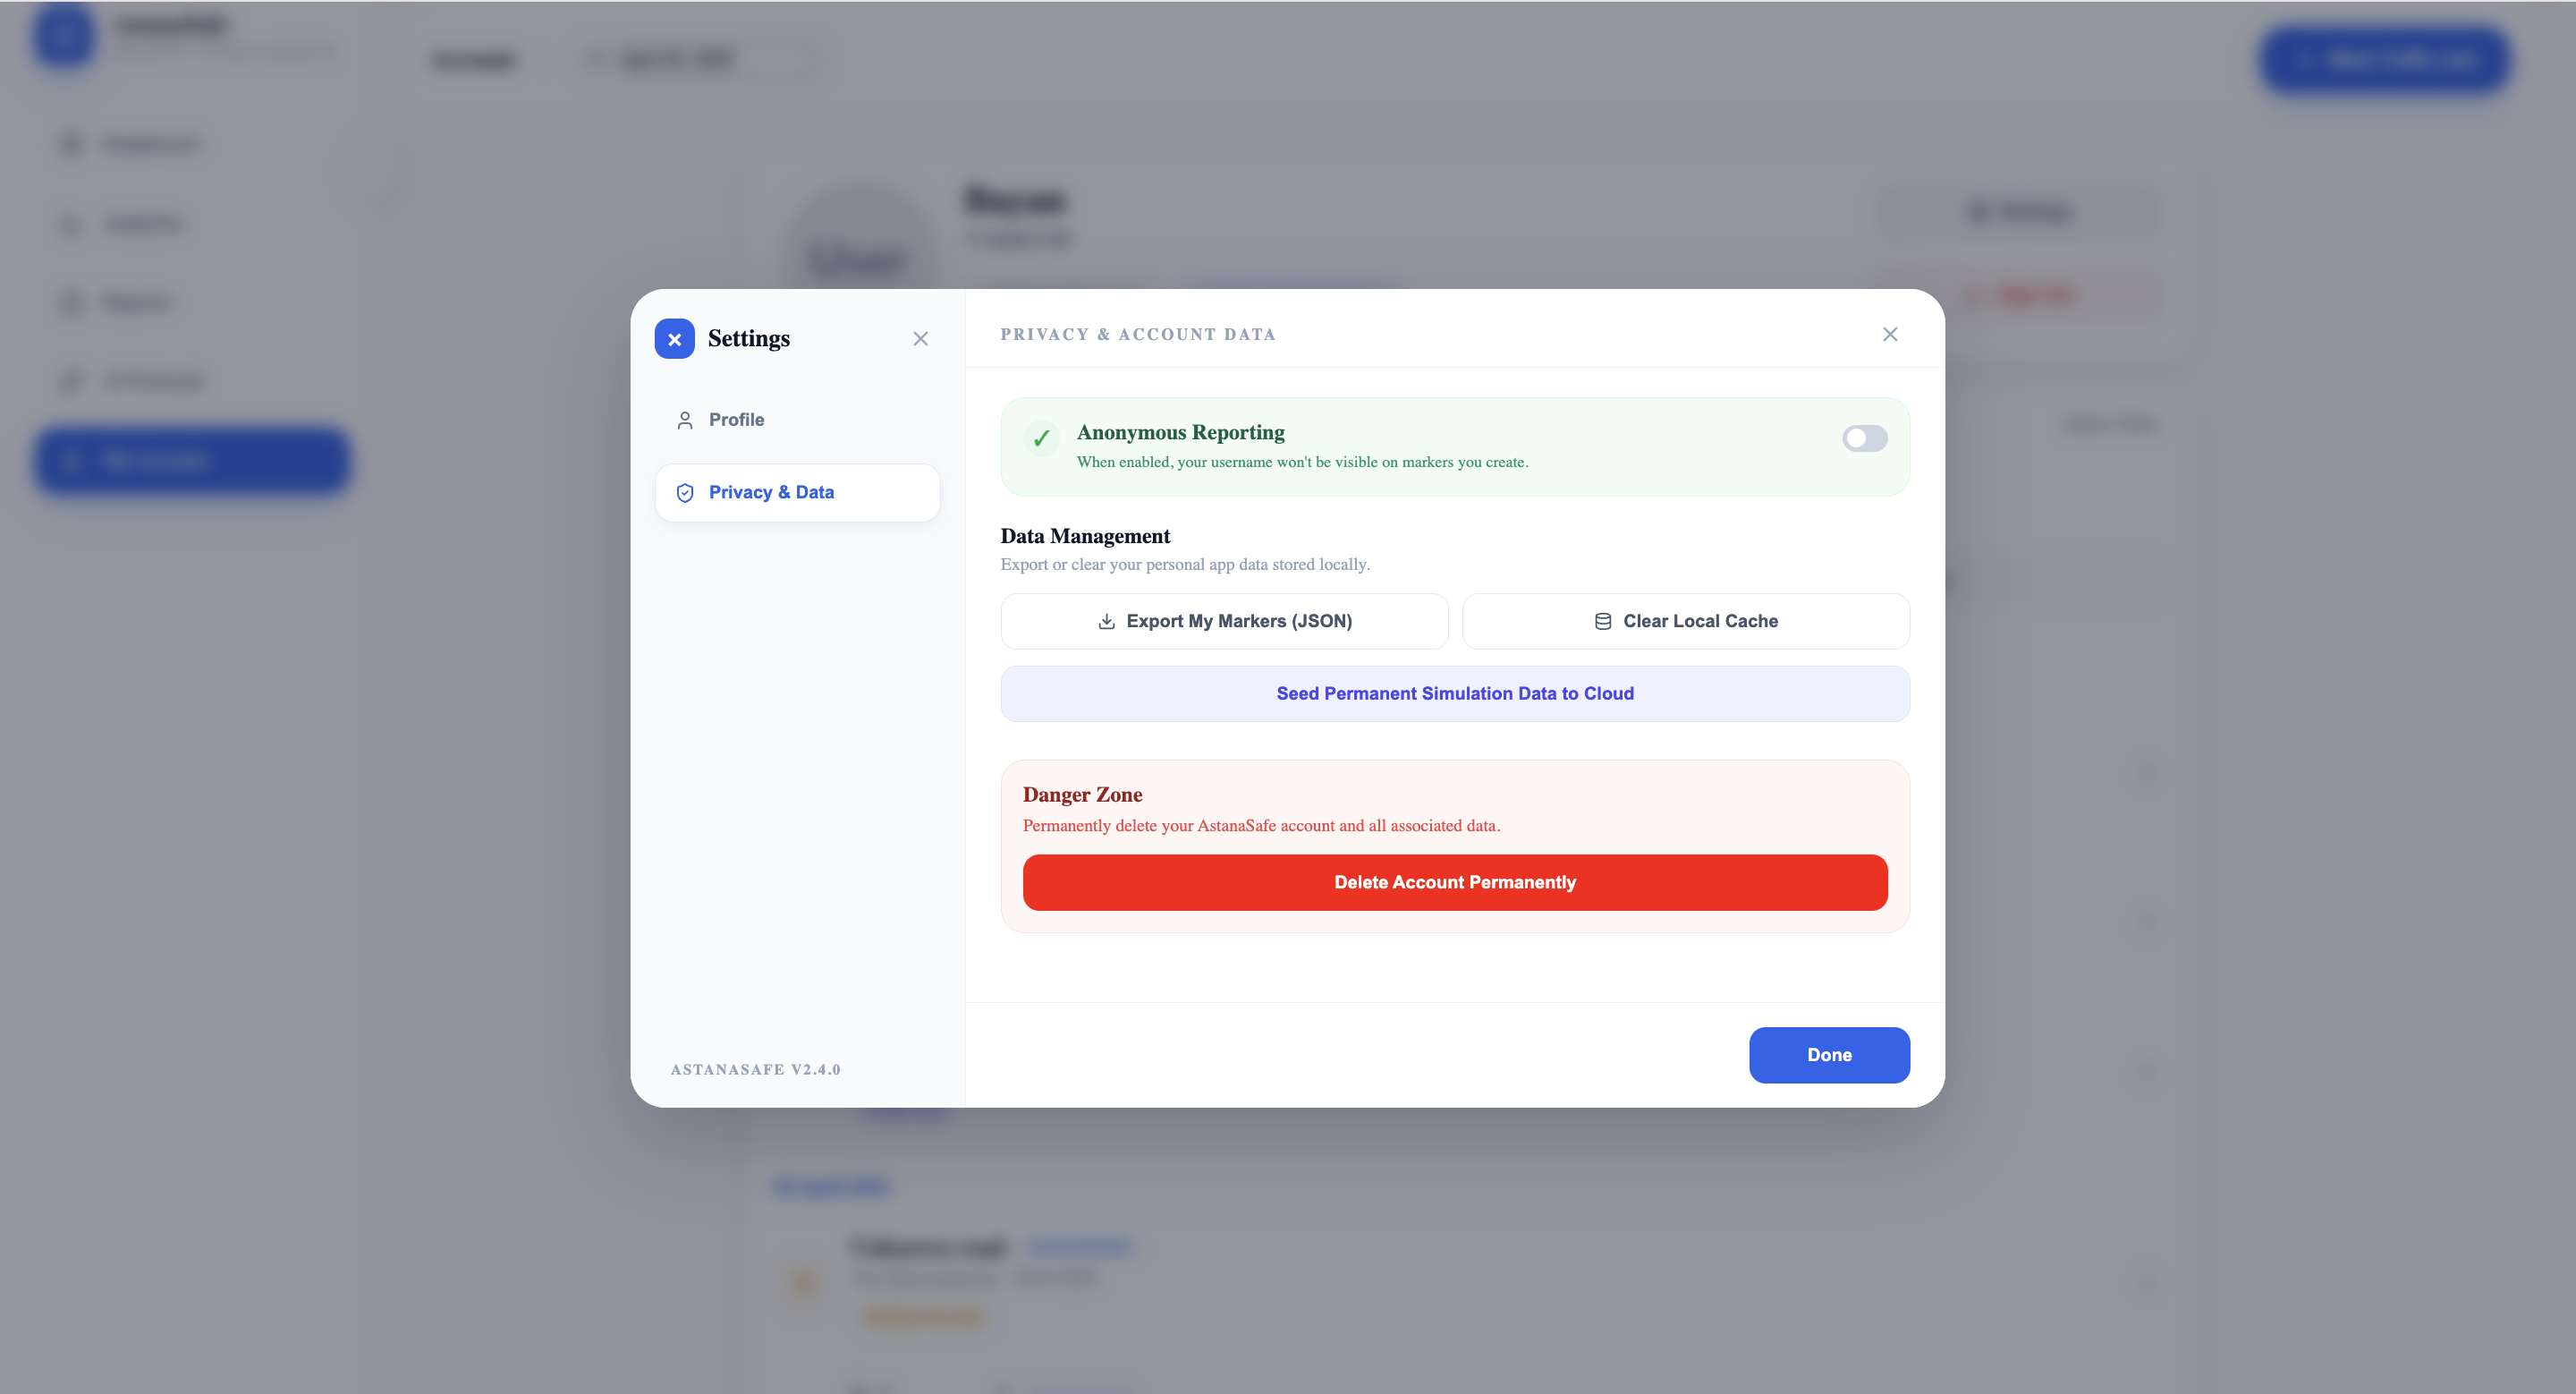
\includegraphics[width=0.75\textwidth]{sc10_settings_privacy.png}
  \caption{\centering Settings modal - Privacy \& Data tab: anonymous reporting toggle, data export and cache controls, and permanent account deletion option.}
  \label{fig:settings_privacy}
\end{figure}

\section{System Testing}

Testing of the AstanaSafe dashboard was conducted manually by the developers throughout the implementation stage, following a test-driven review of each functional requirement after it was implemented. No automated testing framework, continuous integration pipeline, or external user testing programme was employed within the project timeline. The test dataset comprised a combination of seeded accident records loaded into the database for April 2026 and live user-submitted traffic reports created during UI testing sessions, resulting in up to 12 active records visible on the dashboard at a time.

Table~\ref{tab:test_cases} presents the set of test cases executed against the system, along with the expected and actual results observed during testing.

\renewcommand{\arraystretch}{1.4}

\begin{tabularx}{\textwidth}{|p{1.4cm}
                  |p{4cm}
                  |X
                  |p{1.2cm}|}


\hline
\textbf{TC ID} & \textbf{Test Case} & \textbf{Expected and Observed Result} & \textbf{Status} \\
\hline
\endfirsthead

\hline
\textbf{TC ID} & \textbf{Test Case} & \textbf{Expected and Observed Result} & \textbf{Status} \\
\hline
\endhead

    TC-01 & Submit a traffic report via the Mark Traffic Jam modal &
    New marker appears on the map immediately after submission; record stored in database with correct timestamp and weather data &
    Pass \\
    \hline

    TC-02 & Apply district filters (Almaty, Baikonur, Esil, Nura, Saryarka, Sarayshyq) on Dashboard &
    Only records belonging to the selected district are rendered on the map;  
    visible report counter updates accordingly for each district &
    Pass \\
    \hline

    TC-03 & Change global date picker &
    All KPI cards, map markers, and activity log refresh to reflect records for selected date &
    Pass \\
    \hline

    TC-04 & Apply weather filter "Clear" on Dashboard &
    Only records with weather condition "clear" are shown on the map;  
    markers for rain/unknown weather are hidden &
    Pass \\
    \hline

    TC-05 & Open Complete Activity Log &
    Modal displays correct counts: 12 total logs, 9 accidents, 3 traffic jams;  
    search and type filters function correctly &
    Pass \\
    \hline

    TC-06 & Export records as CSV from Reports page &
    CSV file downloads containing all filtered records with correct columns and values &
    Pass \\
    \hline

    TC-07 & Click "View on Map" from Reports table row &
    Application navigates to Dashboard; corresponding map marker is highlighted at correct location &
    Pass \\
    \hline

    TC-08 & Refresh AI Forecast &
    New forecast and risk levels generated based on most recent database records &
    Pass \\
    \hline

    TC-09 & Delete user-submitted report from Account page &
    Report removed from "My Recent Marks"; corresponding map marker disappears from Dashboard &
    Pass \\
    \hline

    TC-10 & Toggle Anonymous Reporting in Settings &
    New submissions do not display user name on public markers; existing data remains unchanged &
    Pass \\
    \hline

  \caption{\centering Manual test cases and results}
  \label{tab:test_cases}
  
\end{tabularx}

All ten test cases passed without defects requiring structural changes to the system. Minor cosmetic adjustments to filter label alignment and modal spacing were addressed during the testing phase but did not affect functional behaviour. The testing results confirm that the core user workflows - report submission, spatial filtering, analytics viewing, forecast generation, and data management - operate as intended with the current test dataset.

The principal limitation of the testing approach is the absence of automated regression testing, which means that future modifications to the codebase cannot be validated against the current behaviour in a systematic way. This limitation is acknowledged as a direction for future development, where the implementation of a unit and integration test suite using frameworks such as pytest and React Testing Library would substantially improve long-term maintainability.

\section{Practical Significance of the Web Dashboard}

The AstanaSafe dashboard addresses a well-defined gap in the current landscape of traffic and road safety information tools available to users in Astana. As established in Chapter 1, existing commercial platforms - 2GIS, Yandex Maps, and Google Maps - provide real-time navigation assistance but do not retain historical incident records, do not support structured user data submission in a research context, and do not offer weather-correlated analytics or district-level comparative analysis. The proposed system fills each of these gaps through a purpose-built analytical interface that uses exclusively open-source components and stores all user-contributed data in a persistent relational database.

For the research and academic community, the dashboard provides an accessible entry point to spatial traffic data analysis. Students and researchers at institutions such as Astana IT University can use the platform to conduct district-level comparisons, investigate temporal incident patterns, and analyse the relationship between weather conditions and accident frequency without requiring GIS software licences or data preprocessing skills. The data export functionality in the Reports module further supports academic workflows by allowing records to be extracted in CSV format for use in external statistical tools.

For urban planners and transport specialists, the combination of the heatmap visualisation, the severity breakdown by district, and the congested arteries ranking provides a structured evidence base for identifying infrastructure priorities. The ability to filter by incident type and severity and to view records across a custom date range allows decision-makers to isolate specific problem categories and compare conditions across different periods.

For general users and commuters, the dashboard offers a clear, visually intuitive view of traffic conditions and safety risks at the city level. The AI Forecast module translates complex data patterns into actionable behavioural advice - reduced speed, increased following distance, district-specific caution - presented in plain language accessible to users without technical backgrounds.

The system is architecturally designed for extensibility. The separation of frontend and backend, the modular router structure in the API, and the use of standardised data formats mean that additional data sources - such as official accident records from government agencies, integration with real-time sensor networks, or extended weather history - can be incorporated without restructuring the existing codebase. The open-source technology stack eliminates licensing barriers for any future developer who wishes to extend, fork, or adapt the platform for other Kazakhstani cities or for academic collaboration. These properties position AstanaSafe as a practical foundation for continued smart-city development in the context of Astana's ongoing urban expansion~\cite{praharaj2022, miranda2024}.






\chapter{Proposed System Improvements}

\subsection*{1. Traffic Jam Module Enhancements}
The traffic jam module will be extended by introducing more detailed classification and filtering options. Severity levels will be added to the incident category, and congestion levels will be introduced for traffic jams. In addition, the system will include expanded incident types, weather conditions, and external factors such as holidays and public events.

\begin{itemize}
    \item Add severity filters in \textit{Incident Category}:
    \begin{itemize}
        \item Low severity accident
        \item Medium severity accident
        \item High severity accident
    \end{itemize}
    
    \item Add congestion level filters in \textit{Traffic Jam Category}:
    \begin{itemize}
        \item Low traffic jam
        \item Medium traffic jam
        \item Active (high) traffic jam
    \end{itemize}
    
    \item Expand incident types:
    \begin{itemize}
        \item Collision
        \item Vehicle breakdown
        \item Road construction
        \item Lane closure
        \item Other additional types
    \end{itemize}
    
    \item Expand contextual factors:
    \begin{itemize}
        \item Weather conditions:
        \begin{itemize}
            \item Rainy
            \item Snowy
            \item Icy
            \item Foggy
            \item Windy
        \end{itemize}
        
        \item External impacts:
        \begin{itemize}
            \item Holidays
            \item Public events
            \item Other city-level factors
        \end{itemize}
    \end{itemize}
\end{itemize}

\subsection*{2. Map Interaction Improvement}
The map interface will be improved by introducing hover-based interaction with markers. When a user points at a traffic object, a small tooltip will appear showing key information. This allows faster access to data without requiring additional clicks.

\begin{itemize}
    \item Add hover-based preview on map markers
    \item Display a small information tooltip when the user points at a marker without clicking
\end{itemize}

\subsection*{3. AI System Extension}
The current AI component based on Gemini will be extended with an additional machine learning layer. This enhancement will allow more advanced data processing and support future analytical features. The combination of approaches will improve system flexibility.

\begin{itemize}
    \item Keep Gemini AI integration
    \item Add an additional Machine Learning layer
\end{itemize}

\subsection*{4. Admin Panel}
An administrative panel will be introduced to manage system data and user-generated content. The admin will be able to review, edit, and remove incorrect entries. This ensures better control over data quality.

\begin{itemize}
    \item Add admin account functionality
    \item Enable editing of user-submitted markers
    \item Enable deletion of incorrect or misleading reports
\end{itemize}

\subsection*{5. Fake Information Control}
A trust-based system will be implemented to reduce the impact of incorrect data. Users will be evaluated based on the accuracy of their previous submissions. This allows prioritization of reliable contributors.

\begin{itemize}
    \item Add user trust/reputation system
    \item Track accuracy of user submissions
    \item Prioritize trusted users
\end{itemize}

\subsection*{6. Progressive Web App (PWA)}
The system will be adapted to function as a Progressive Web App. This will allow users to install the application on mobile devices. The interface will remain accessible across different platforms.

\begin{itemize}
    \item Enable installation on mobile devices
    \item Add PWA support for the web dashboard
\end{itemize}

\subsection*{7. Data Export}
A data export feature will be added to support external usage of system data. Users will be able to download information in structured formats. This enables integration with other tools.

\begin{itemize}
    \item Add export functionality:
    \begin{itemize}
        \item PDF format
        \item CSV format
    \end{itemize}
\end{itemize}

\subsection*{8. UI/UX Improvements}
The user interface will be enhanced to improve usability and visual consistency. Additional animations and design refinements will be introduced. These changes will make interaction smoother.

\begin{itemize}
    \item Improve animations
    \item Improve overall design
\end{itemize}

\subsection*{9. Reports Page Update}
The reports page will be extended with more flexible filtering options. Instead of only date-based filters, additional parameters will be introduced. This allows more detailed analysis of historical data.

\begin{itemize}
    \item Replace current filters (day, month, year)
    \item Add new filters:
    \begin{itemize}
        \item Time
        \item Day
        \item Month
        \item Category
    \end{itemize}
\end{itemize}

\subsection*{10. Data and Database Description}
A detailed description of data sources will be included in the system documentation. The database structure and organization will also be explained. This ensures transparency of data handling.

\begin{itemize}
    \item Add description of data sources
    \item Add database description
    \item Add database structure explanation
\end{itemize}

\subsection*{11. System Testing}
The system testing process will be formally described. This includes validation of functionality and performance. Testing ensures system reliability.

\begin{itemize}
    \item Add description of system testing process
\end{itemize}

\subsection*{12. Expert Validation}
Expert feedback will be incorporated into the system evaluation. This includes opinions from TODD and Zeret. Their input will support validation of system effectiveness.

\begin{itemize}
    \item Add expert opinion (TODD)
    \item Add Zeret evaluation/feedback
\end{itemize}

% ============================================================
% CONCLUSION
% ============================================================
\chapter*{Conclusion}
\addcontentsline{toc}{chapter}{Conclusion}

The present project addressed a well-defined gap in the landscape of traffic
information tools available to users in Astana: the absence of a publicly accessible,
analytically capable platform for exploring spatial and temporal patterns in road
accidents and congestion. In response to this gap, the work set out to design and
implement a web-based dashboard - AstanaSafe - integrating interactive mapping,
structured incident reporting, multi-dimensional analytics, and an AI-powered safety
forecast into a coherent interface accessible to specialist and non-specialist users
alike.
 
\textbf{Fulfilment of objectives.} All five project objectives defined in Section~1.1 were achieved. A systematic review confirmed that existing commercial tools - 2GIS, Yandex Maps, and Google Maps - serve as navigation assistants rather than analytical systems. The system architecture was specified as a client-server application with clearly delineated layers and a documented REST API. The interactive mapping interface was implemented using Leaflet and OpenStreetMap, supporting colour-coded incident submission with full metadata. The analytical module delivers hourly distribution, severity breakdowns, congested arteries ranking, and weather impact views. Functional testing across ten test cases confirmed that all core workflows operate correctly.

\textbf{Research findings.} Semi-structured interviews with 19 participants across four stakeholder segments identified data fragmentation as the primary shared barrier. Interactive maps were the most universally requested feature, temporal and district filtering was considered essential by all user groups, and interface accessibility for non-technical audiences emerged as equally important as analytical depth. Weather context was raised independently by multiple segments, validating the decision to integrate the Open-Meteo API.

\textbf{Significance of the developed system.} AstanaSafe demonstrates that a single open-source dashboard can serve multiple user communities. Researchers gain a structured, exportable incident dataset without requiring GIS skills; planners gain a spatial evidence base for infrastructure prioritisation; and commuters receive plain-language safety advice through the AI Forecast module. The fully open-source stack allows the platform to be extended or adapted for other cities without licensing constraints.

\textbf{Limitations.} The system lacks an automated regression testing suite, limiting validation of future code changes. The AI forecast relies on rule-based generation rather than a trained model, and the database remains on SQLite pending migration to PostgreSQL. The analytical value of the crowdsourced archive will grow only as the contributor base expands.

\textbf{Future directions.} Chapter~3 outlines twelve proposed improvements, including a machine learning forecasting layer, an administrative panel, a user trust and reputation system, and Progressive Web App support. Together these enhancements would advance AstanaSafe from a working prototype to a production-grade platform suitable for deployment by municipal authorities across Kazakhstan.

\clearpage

% ============================================================
% BIBLIOGRAPHY
% ============================================================

\begin{thebibliography}{99}
\addcontentsline{toc}{chapter}{Bibliography}

\bibitem{who2023}
World Health Organization. (2023). \textit{Global status report on road
safety 2023}. WHO Press.
\href{https://www.who.int/publications/i/item/9789240086517}
{https://www.who.int/publications/i/item/9789240086517}

\bibitem{kzstat2023}
Bureau of National Statistics of the Agency for Strategic Planning and
Reforms of the Republic of Kazakhstan. (2023). \textit{Statistical
yearbook: Kazakhstan in figures 2023}.
\href{https://stat.gov.kz/en/}{https://stat.gov.kz/en/}

\bibitem{endashaw2025}
Endashaw, D.~K., Habtegiorgis, K.~A., Al-Ramadan, B.~M., Al-Ahmadi,
H.~M., \& Deressa, B.~F. (2025). A systematic review on GIS-based road
traffic accidents analysis and road safety audit.
\textit{Computational Urban Science}, \textit{5}, 53.
\href{https://doi.org/10.1007/s43762-025-00221-w}
{https://doi.org/10.1007/s43762-025-00221-w}

\bibitem{salameh2024}
Alsahfi, T. (2024). Spatial and temporal analysis of road traffic
accidents in major Californian cities using a geographic information
system. \textit{ISPRS International Journal of Geo-Information},
\textit{13}(5), 157.
\href{https://doi.org/10.3390/ijgi13050157}
{https://doi.org/10.3390/ijgi13050157}

\bibitem{oecd2022}
Organisation for Economic Co-operation and Development / International
Transport Forum. (2022). \textit{Road safety annual report 2022}.
OECD Publishing.
\href{https://www.itf-oecd.org/sites/default/files/docs/irtad-road-safety-annual-report-2022.pdf}
{https://www.itf-oecd.org/sites/default/files/docs/irtad-road-safety-annual-report-2022.pdf}

\bibitem{becker2022}
Becker, N., Rust, H.~W., \& Ulbrich, U. (2022). Weather impacts on
various types of road crashes: a quantitative analysis using generalized
additive models. \textit{European Transport Research Review},
\textit{14}, 37.
\href{https://doi.org/10.1186/s12544-022-00561-2}
{https://doi.org/10.1186/s12544-022-00561-2}

\bibitem{liang2023}
Liang, C.~W., Chang, C.~C., \& Liang, J.~J. (2023). The impacts of
air quality and secondary organic aerosols formation on traffic accidents
in heavy fog-haze weather. \textit{Heliyon}, \textit{9}(4), e14631.
\href{https://doi.org/10.1016/j.heliyon.2023.e14631}
{https://doi.org/10.1016/j.heliyon.2023.e14631}

\bibitem{janez2022}
Jane\v{z}, M., Verov\v{s}ek, \v{S}., Zupan\v{c}i\v{c}, T., \&
Mo\v{s}kon, M. (2022). Citizen science for traffic monitoring:
investigating the potentials for complementing traffic counters with
crowdsourced data. \textit{Sustainability}, \textit{14}(2), 622.
\href{https://doi.org/10.3390/su14020622}
{https://doi.org/10.3390/su14020622}

\bibitem{herfort2021}
Herfort, B., Lautenbach, S., Porto de Albuquerque, J., Anderson, J.,
\& Zipf, A. (2021). The evolution of humanitarian mapping within the
OpenStreetMap community. \textit{Scientific Reports}, \textit{11},
3037.
\href{https://doi.org/10.1038/s41598-021-82404-z}
{https://doi.org/10.1038/s41598-021-82404-z}

\bibitem{tzavella2022}
Tzavella, K., Skopeliti, A., \& Fekete, A. (2024). Volunteered geographic
information use in crisis, emergency and disaster management: a scoping
review and a web atlas. \textit{Geo-spatial Information Science},
\textit{27} (2), 423-454.
\href{https://doi.org/10.1080/10095020.2022.2139642}
{https://doi.org/10.1080/10095020.2022.2139642}

\bibitem{praharaj2022}
Praharaj, S., Solis, P., \& Wentz, E. A. (2022). Deploying geospatial visualization
dashboards to combat the socioeconomic impacts of COVID-19.
\textit{Environment and Planning B: Urban Analytics and City Science},
\textit{50}(5), 1262-1279.
\href{https://doi.org/10.1177/23998083221142863}
{https://doi.org/10.1177/23998083221142863}

\bibitem{miranda2024}
Miranda, F., Ortner, T., Moreira, G., Hosseini, M., Vuckovic, M., Biljecki, F., Silva, C.T., Lage, M. and Ferreira, N. (2024). The state of the art in visual
analytics for 3D urban data. \textit{Computer Graphics Forum},
\textit{43}(3), e15112.
\href{https://doi.org/10.1111/cgf.15112}
{https://doi.org/10.1111/cgf.15112}

\bibitem{osm2024}
OpenStreetMap contributors. (2024). \textit{OpenStreetMap}.
OpenStreetMap Foundation.
\href{https://www.openstreetmap.org}{https://www.openstreetmap.org}

\bibitem{openmeteo2023}
Zippenfenig, P. (2023). \textit{Open-Meteo.com weather API} [Data
set]. Zenodo.
\href{https://doi.org/10.5281/zenodo.7970649}
{https://doi.org/10.5281/zenodo.7970649}

\bibitem{fastapi2024}
Ramirez, S. (2024). \textit{FastAPI documentation: Modern, fast
(high-performance) web framework for building APIs with Python}.
\href{https://fastapi.tiangolo.com}{https://fastapi.tiangolo.com}


\bibitem{swebok2014}
Washizaki, H. (eds.,). (2024). \textit{Guide to the Software Engineering Body of Knowledge (SWEBOK Guide) Version 4.0}. IEEE Computer Society. \url{https://www.computer.org/education/bodies-of-knowledge/software-engineering}

\bibitem{iso25010}
Sheppard, E. (2025). ISO/IEC 25010:2023 Systems and software engineering - Systems and software Quality Requirements and Evaluation (SQuaRE) - Product quality model characteristics, sub-characteristics, definitions, and their proposed application to electric vehicle supply equipment (EVSE) software.  \textit{}. Zenodo. \url{https://doi.org/10.5281/zenodo.14758339}

\bibitem{react2024}
Meta Open Source. (2024). \textit{React: The library for web and native user interfaces}. \url{https://react.dev}

\bibitem{vitejs2024}
You, E., \& Vite contributors. (2024). \textit{Vite: Next generation frontend tooling}. \url{https://vitejs.dev/}

\bibitem{leaflet2024}
Agafonkin, V. (2024). \textit{Leaflet: An open-source JavaScript library for mobile-friendly interactive maps}. \url{https://leafletjs.com}


\bibitem{chartjs2024}
Chart.js contributors. (2024). \textit{Chart.js documentation: Simple yet flexible JavaScript charting library}. \url{https://www.chartjs.org/docs/latest/}

\bibitem{pydantic2024}
Colvin, S. (2024). \textit{Pydantic documentation: Data validation using Python type hints}. \url{https://docs.pydantic.dev/}

\bibitem{sqlalchemy2024}
Bayer, M. (2024). \textit{SQLAlchemy: The Python SQL toolkit and object relational mapper}. \url{https://www.sqlalchemy.org/}

\bibitem{postgresql2024}
PostgreSQL Global Development Group. (2024). \textit{PostgreSQL 16 documentation}. \url{https://www.postgresql.org/docs/}

\bibitem{yin2021}
Yin, X., Wu, G., Wei, J., Shen, Y., Qi, H., \& Yin, B. (2022). Deep learning on traffic Prediction: methods, analysis, and future directions.\textit{IEEE Transactions on Intelligent Transportation Systems,}, \textit{23}(6), 4927-4943. \url{https://doi.org/10.1109/tits.2021.3054840}

\bibitem{shu2023}
Shu, L., \& Zheng, D. (2023). Exploring the application of big data visualization platform in urban traffic data analysis. \textit{Journal of Global Humanities and Social Sciences}, \textit{4}, 176-180. \url{https://doi.org/10.61360/BoniGHSS232014170805}

\bibitem{guo2024}
Kim, J., Jeon, W., \& Kim, S. (2024). Analyzing the relationship between user feedback and traffic accidents through crowdsourced data. \textit{Sustainability}, \textit{16}(22), 9867. \url{https://doi.org/10.3390/su16229867}

\end{thebibliography}

% ============================================================
%  APPENDICES  —  paste after Chapter 3, before \end{document}
%  Requires \usepackage{subcaption} in your preamble
% ============================================================

\appendix

% -----------------------------------------------------------
%  APPENDIX A — INTERVIEW EVIDENCE
% -----------------------------------------------------------

\chapter*{Appendix A}
\addcontentsline{toc}{chapter}{Appendix A}

\section*{Interview Evidence: Segment A and Segment~B}
\addcontentsline{toc}{section}{Interview Evidence: Segment A and Segment~B}
\label{app:interviews}

This appendix presents screenshot evidence from the semi-structured interviews
conducted in January 2026 with participants belonging to Stakeholder Segments~A
and~B. For each respondent, four consecutive screenshots document the interview
session in chronological order. Stakeholder Segments~C (urban planners and
researchers) and D (drivers and commuters) participated via audio recording only;
no visual evidence is included for those segments.

% -----------------------------------------------------------
%  SEGMENT A
% -----------------------------------------------------------

\section*{Segment A - City Transport and Road Infrastructure Specialists}
\addcontentsline{toc}{section}{Segment A - Transport and Road Infrastructure Specialists}

Segment~A comprised students and professionals with expertise in urban mobility,
transport engineering, and road safety policy. Respondents were asked about their
current data sources, the attributes they consider most critical, and the analytical
features they would prioritise in a dedicated traffic dashboard.

% ---- A / Respondent 1 -----------------------------------------------

\subsection*{Respondent A1 - Transport Engineering Student}
\addcontentsline{toc}{subsection}{Respondent A1: Transport Engineering Student}

\begin{figure}[H]
\centering
\begin{subfigure}{0.48\textwidth}
    \centering
    
\includegraphics[height=0.32\textheight, keepaspectratio]{1.1.png}
\end{subfigure}
\hfill
\begin{subfigure}{0.48\textwidth}
    \centering
    
\includegraphics[height=0.32\textheight, keepaspectratio]{1.2.png}
\end{subfigure}

\vspace{0.3cm}

\begin{subfigure}{0.48\textwidth}
    \centering
    
\includegraphics[height=0.32\textheight, keepaspectratio]{1.3.png}
\end{subfigure}
\hfill
\begin{subfigure}{0.48\textwidth}
    \centering
    
\includegraphics[height=0.32\textheight, keepaspectratio]{1.4.png}
\end{subfigure}

\caption{\centering Interview with Respondent A1}
\end{figure}

% ---- A / Respondent 2 -----------------------------------------------

\subsection*{Respondent A2 - Urban Planning Student}
\addcontentsline{toc}{subsection}{Respondent A2: Urban Planning Student}

\begin{figure}[H]
\centering
\begin{subfigure}{0.48\textwidth}
    \centering
    
\includegraphics[height=0.32\textheight, keepaspectratio]{2.1.png}
\end{subfigure}
\hfill
\begin{subfigure}{0.48\textwidth}
    \centering
    
\includegraphics[height=0.32\textheight, keepaspectratio]{2.2.png}
\end{subfigure}

\vspace{0.3cm}

\begin{subfigure}{0.48\textwidth}
    \centering
    
\includegraphics[height=0.32\textheight, keepaspectratio]{2.3.png}
\end{subfigure}
\hfill
\begin{subfigure}{0.48\textwidth}
    \centering
    
\includegraphics[height=0.32\textheight, keepaspectratio]{2.4.png}
\end{subfigure}

\caption{\centering Interview with Respondent A2 }
\end{figure}

% ---- A / Respondent 3 -----------------------------------------------

\subsection*{Respondent A3 - Road Infrastructure Intern}
\addcontentsline{toc}{subsection}{Respondent A3: Road Infrastructure Intern}

\begin{figure}[H]
\centering

% верх (3)
\begin{subfigure}{0.32\textwidth}
    \centering
    
\includegraphics[height=0.28\textheight, keepaspectratio]{3.1.png}
\end{subfigure}
\hfill
\begin{subfigure}{0.32\textwidth}
    \centering
    
\includegraphics[height=0.28\textheight, keepaspectratio]{3.2.png}
\end{subfigure}
\hfill
\begin{subfigure}{0.32\textwidth}
    \centering
    
\includegraphics[height=0.28\textheight, keepaspectratio]{3.3.png}
\end{subfigure}

\vspace{0.3cm}

% низ (2)
\begin{subfigure}{0.32\textwidth}
    \centering
    
\includegraphics[height=0.28\textheight, keepaspectratio]{3.4.png}
\end{subfigure}
\hfill
\begin{subfigure}{0.32\textwidth}
    \centering
    
\includegraphics[height=0.28\textheight, keepaspectratio]{3.5.png}
\end{subfigure}

\caption{\centering Interview with Respondent A3}
\end{figure}

% -----------------------------------------------------------
%  SEGMENT B
% -----------------------------------------------------------

\section*{Segment B - Monitoring and Dispatch Users}
\addcontentsline{toc}{section}{Segment B - Monitoring and Dispatch Users}

Segment~B comprised personnel familiar with call-centre and dispatch operations,
including participants with experience in iKOMEK-type monitoring environments.
Respondents were asked about their information channels, the data attributes most
critical during active operations, and the features they would value in a centralised
incident dashboard.

% ---- B / Respondent 1 -----------------------------------------------

\subsection*{Respondent B1 - Call Centre / Monitoring Student}
\addcontentsline{toc}{subsection}{Respondent B1: Call Centre / Monitoring Student}

\begin{figure}[H]
\centering
\begin{subfigure}{0.48\textwidth}
    \centering
    
\includegraphics[height=0.32\textheight, keepaspectratio]{4.1.png}
\end{subfigure}
\hfill
\begin{subfigure}{0.48\textwidth}
    \centering
    
\includegraphics[height=0.32\textheight, keepaspectratio]{4.2.png}
\end{subfigure}

\vspace{0.3cm}

\begin{subfigure}{0.48\textwidth}
    \centering
    
\includegraphics[height=0.32\textheight, keepaspectratio]{4.3.png}
\end{subfigure}
\hfill
\begin{subfigure}{0.48\textwidth}
    \centering
    
\includegraphics[height=0.32\textheight, keepaspectratio]{4.4.png}
\end{subfigure}

\caption{\centering Interview with Respondent B1 }
\end{figure}

% ---- B / Respondent 2 -----------------------------------------------

\subsection*{Respondent B2 - Public Service Dispatch Intern}
\addcontentsline{toc}{subsection}{Respondent B2: Public Service Dispatch Intern}

\begin{figure}[H]
\centering

% верх (3)
\begin{subfigure}{0.32\textwidth}
    \centering
    
\includegraphics[height=0.28\textheight, keepaspectratio]{5.1.png}
\end{subfigure}
\hfill
\begin{subfigure}{0.32\textwidth}
    \centering
    
\includegraphics[height=0.28\textheight, keepaspectratio]{5.2.png}
\end{subfigure}
\hfill
\begin{subfigure}{0.32\textwidth}
    \centering
    
\includegraphics[height=0.28\textheight, keepaspectratio]{5.3.png}
\end{subfigure}

\vspace{0.3cm}

% низ (2)
\begin{subfigure}{0.32\textwidth}
    \centering
    
\includegraphics[height=0.28\textheight, keepaspectratio]{5.4.png}
\end{subfigure}
\hfill
\begin{subfigure}{0.32\textwidth}
    \centering
    
\includegraphics[height=0.28\textheight, keepaspectratio]{5.5.png}
\end{subfigure}

\caption{\centering Interview with Respondent B2}
\end{figure}

% -----------------------------------------------------------
%  Note on Segments C and D
% -----------------------------------------------------------

\section*{Note on Segments C and D}
\addcontentsline{toc}{section}{Note on Segments C and D}

Interviews with Segment~C participants (urban planners and researchers) and
Segment~D participants (drivers and commuters) were conducted in audio format only.
Participants in these segments did not consent to or were unavailable for
screen-recorded sessions. Their contributions are reflected in the narrative and
quantitative analysis presented in Sections~1.4.3 and~1.4.4 of the thesis.


% -----------------------------------------------------------
%  APPENDIX B — SYSTEM INTERFACE FIGURES
% -----------------------------------------------------------
\appendix

% -----------------------------------------------------------
%  APPENDIX A — INTERVIEW EVIDENCE
% -----------------------------------------------------------

\chapter*{Appendix B}
\addcontentsline{toc}{chapter}{Appendix B}
\section* {System Interface Screenshots}
\label{app:screenshots}

This appendix collects all system interface screenshots produced during the
functional testing phase of the AstanaSafe dashboard. The screenshots document
the visual state of each page and module for the test session dated April~20, 2026.
All figures are reproduced at full page width for legibility.

\begin{figure}[H]
  \centering
  \addcontentsline{toc}{subsection}{Figure 6}
  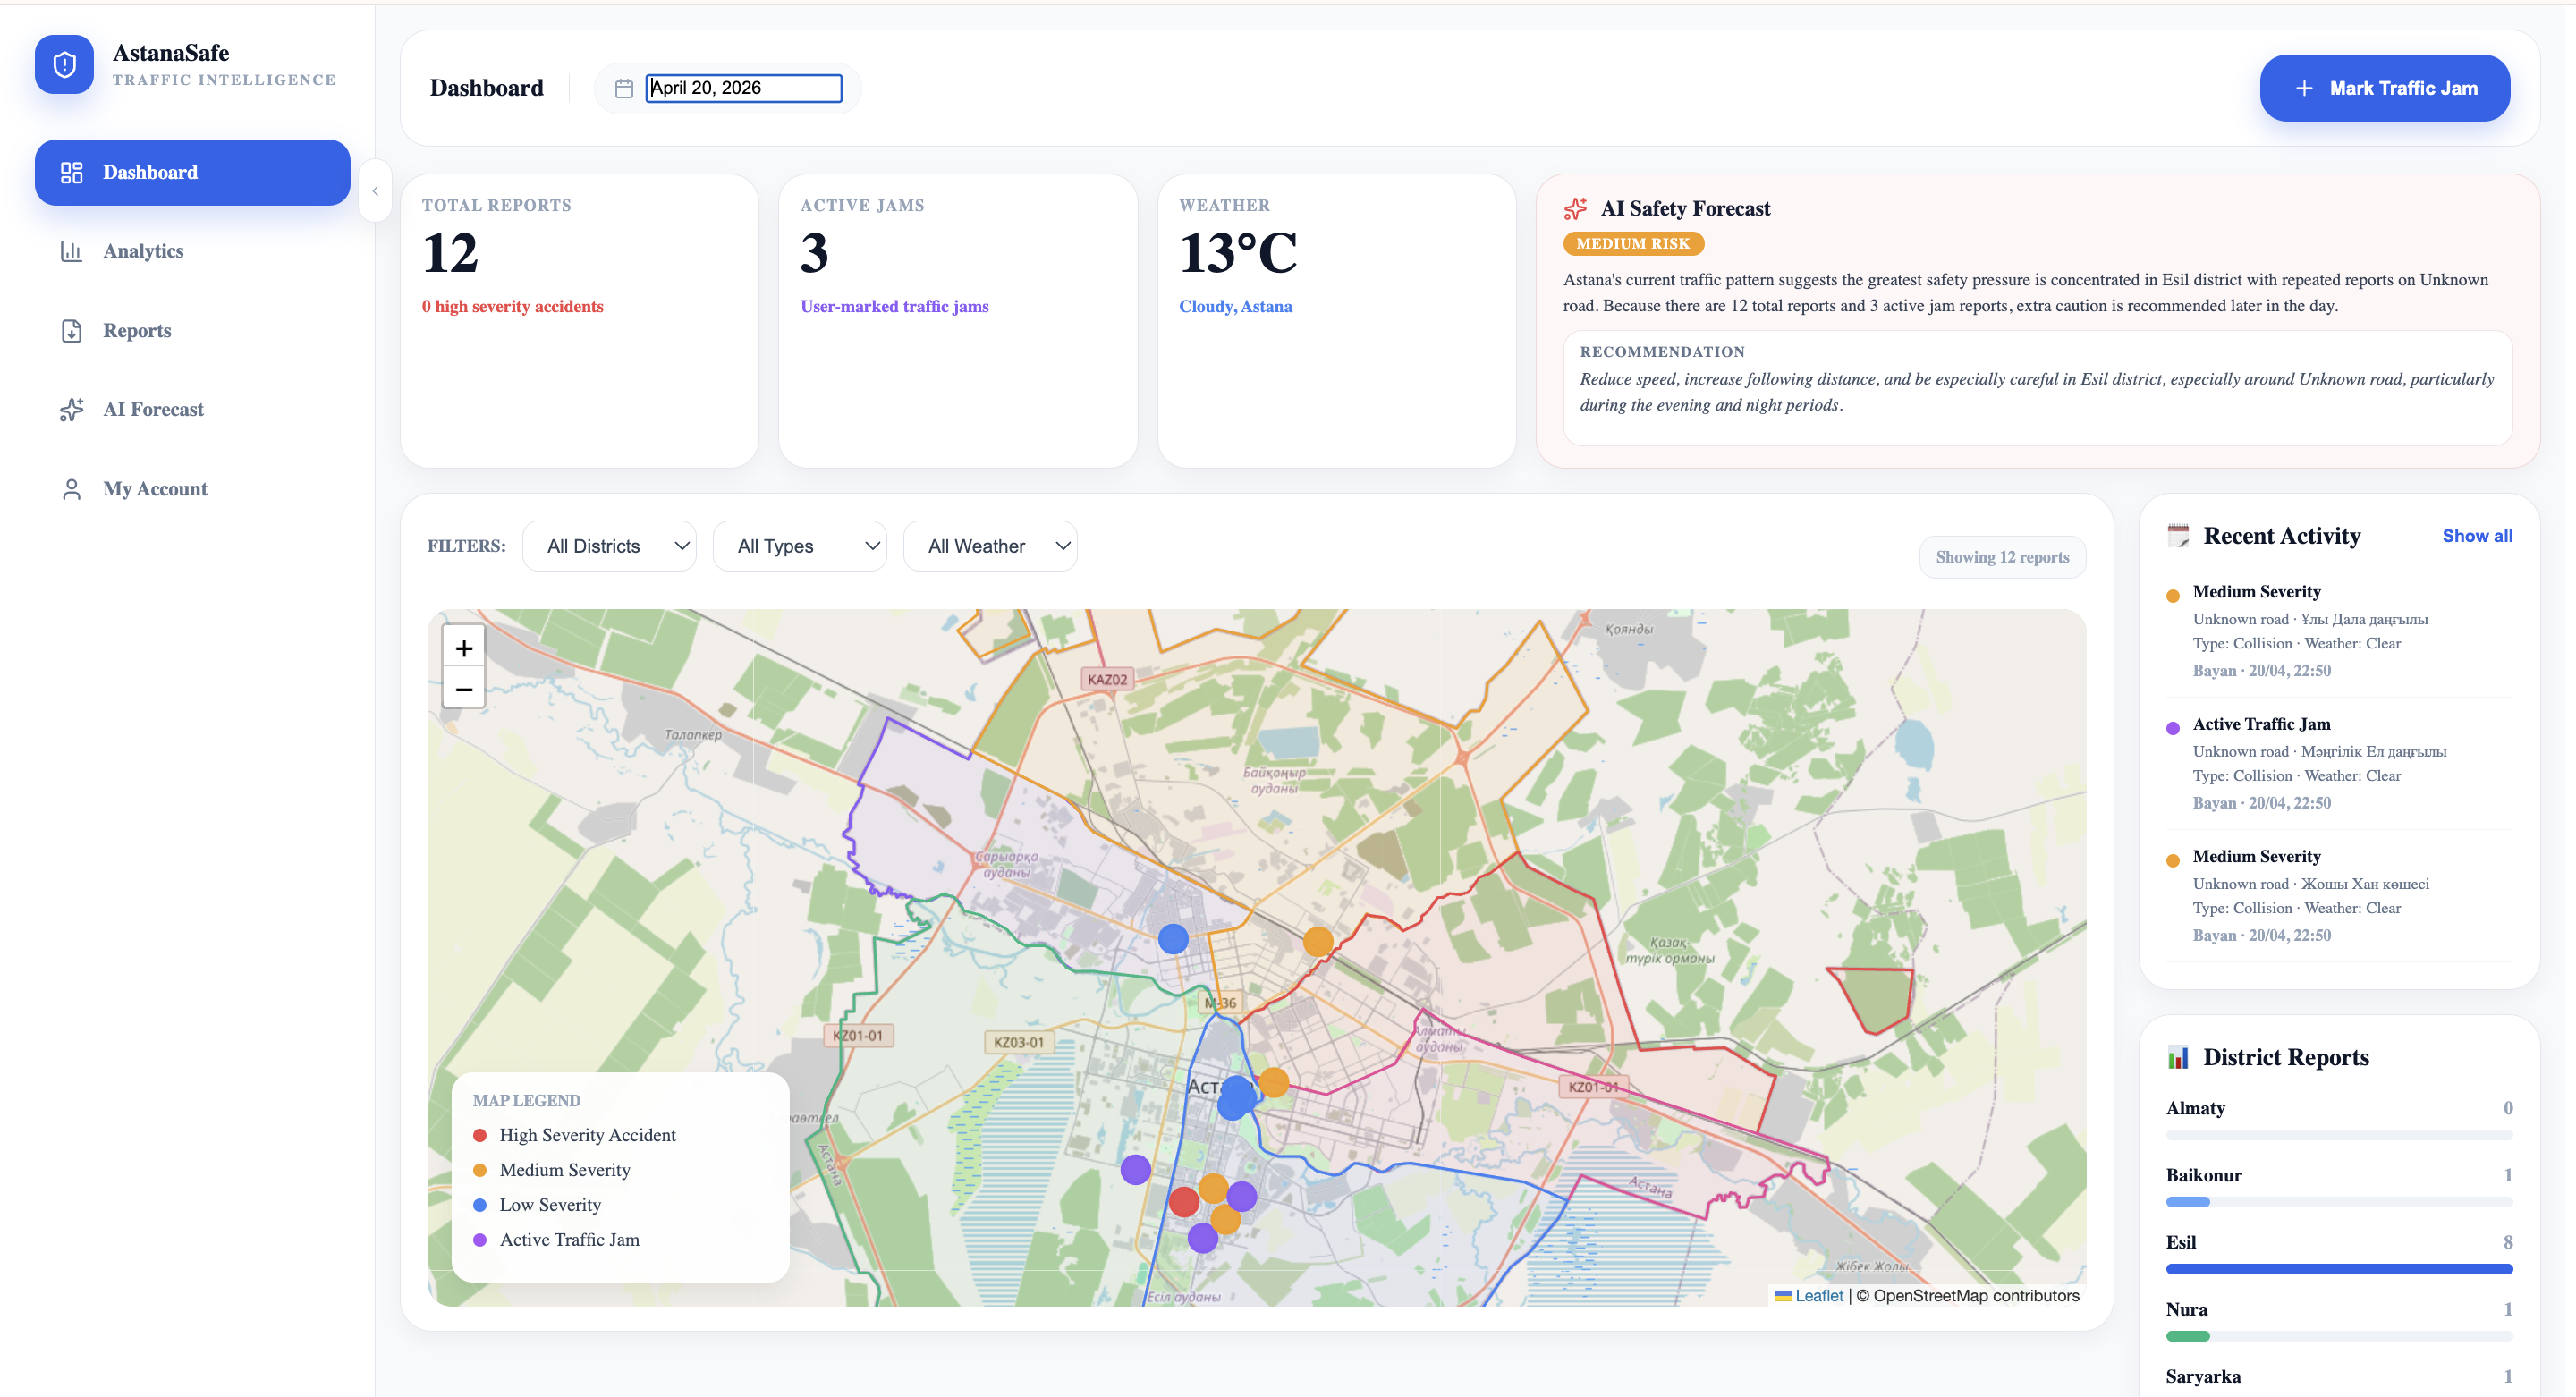
\includegraphics[width=\textwidth]{sc1_dashboard}
  \caption{\centering AstanaSafe Dashboard page displaying KPI summary cards,
           the interactive incident map with colour-coded severity markers and
           district boundary overlays, the Recent Activity timeline panel,
           and the District Reports proportional bar panel.}
  \label{fig:app_dashboard}
\end{figure}

\begin{figure}[H]
  \centering
  \addcontentsline{toc}{subsection}{Figure 7}
  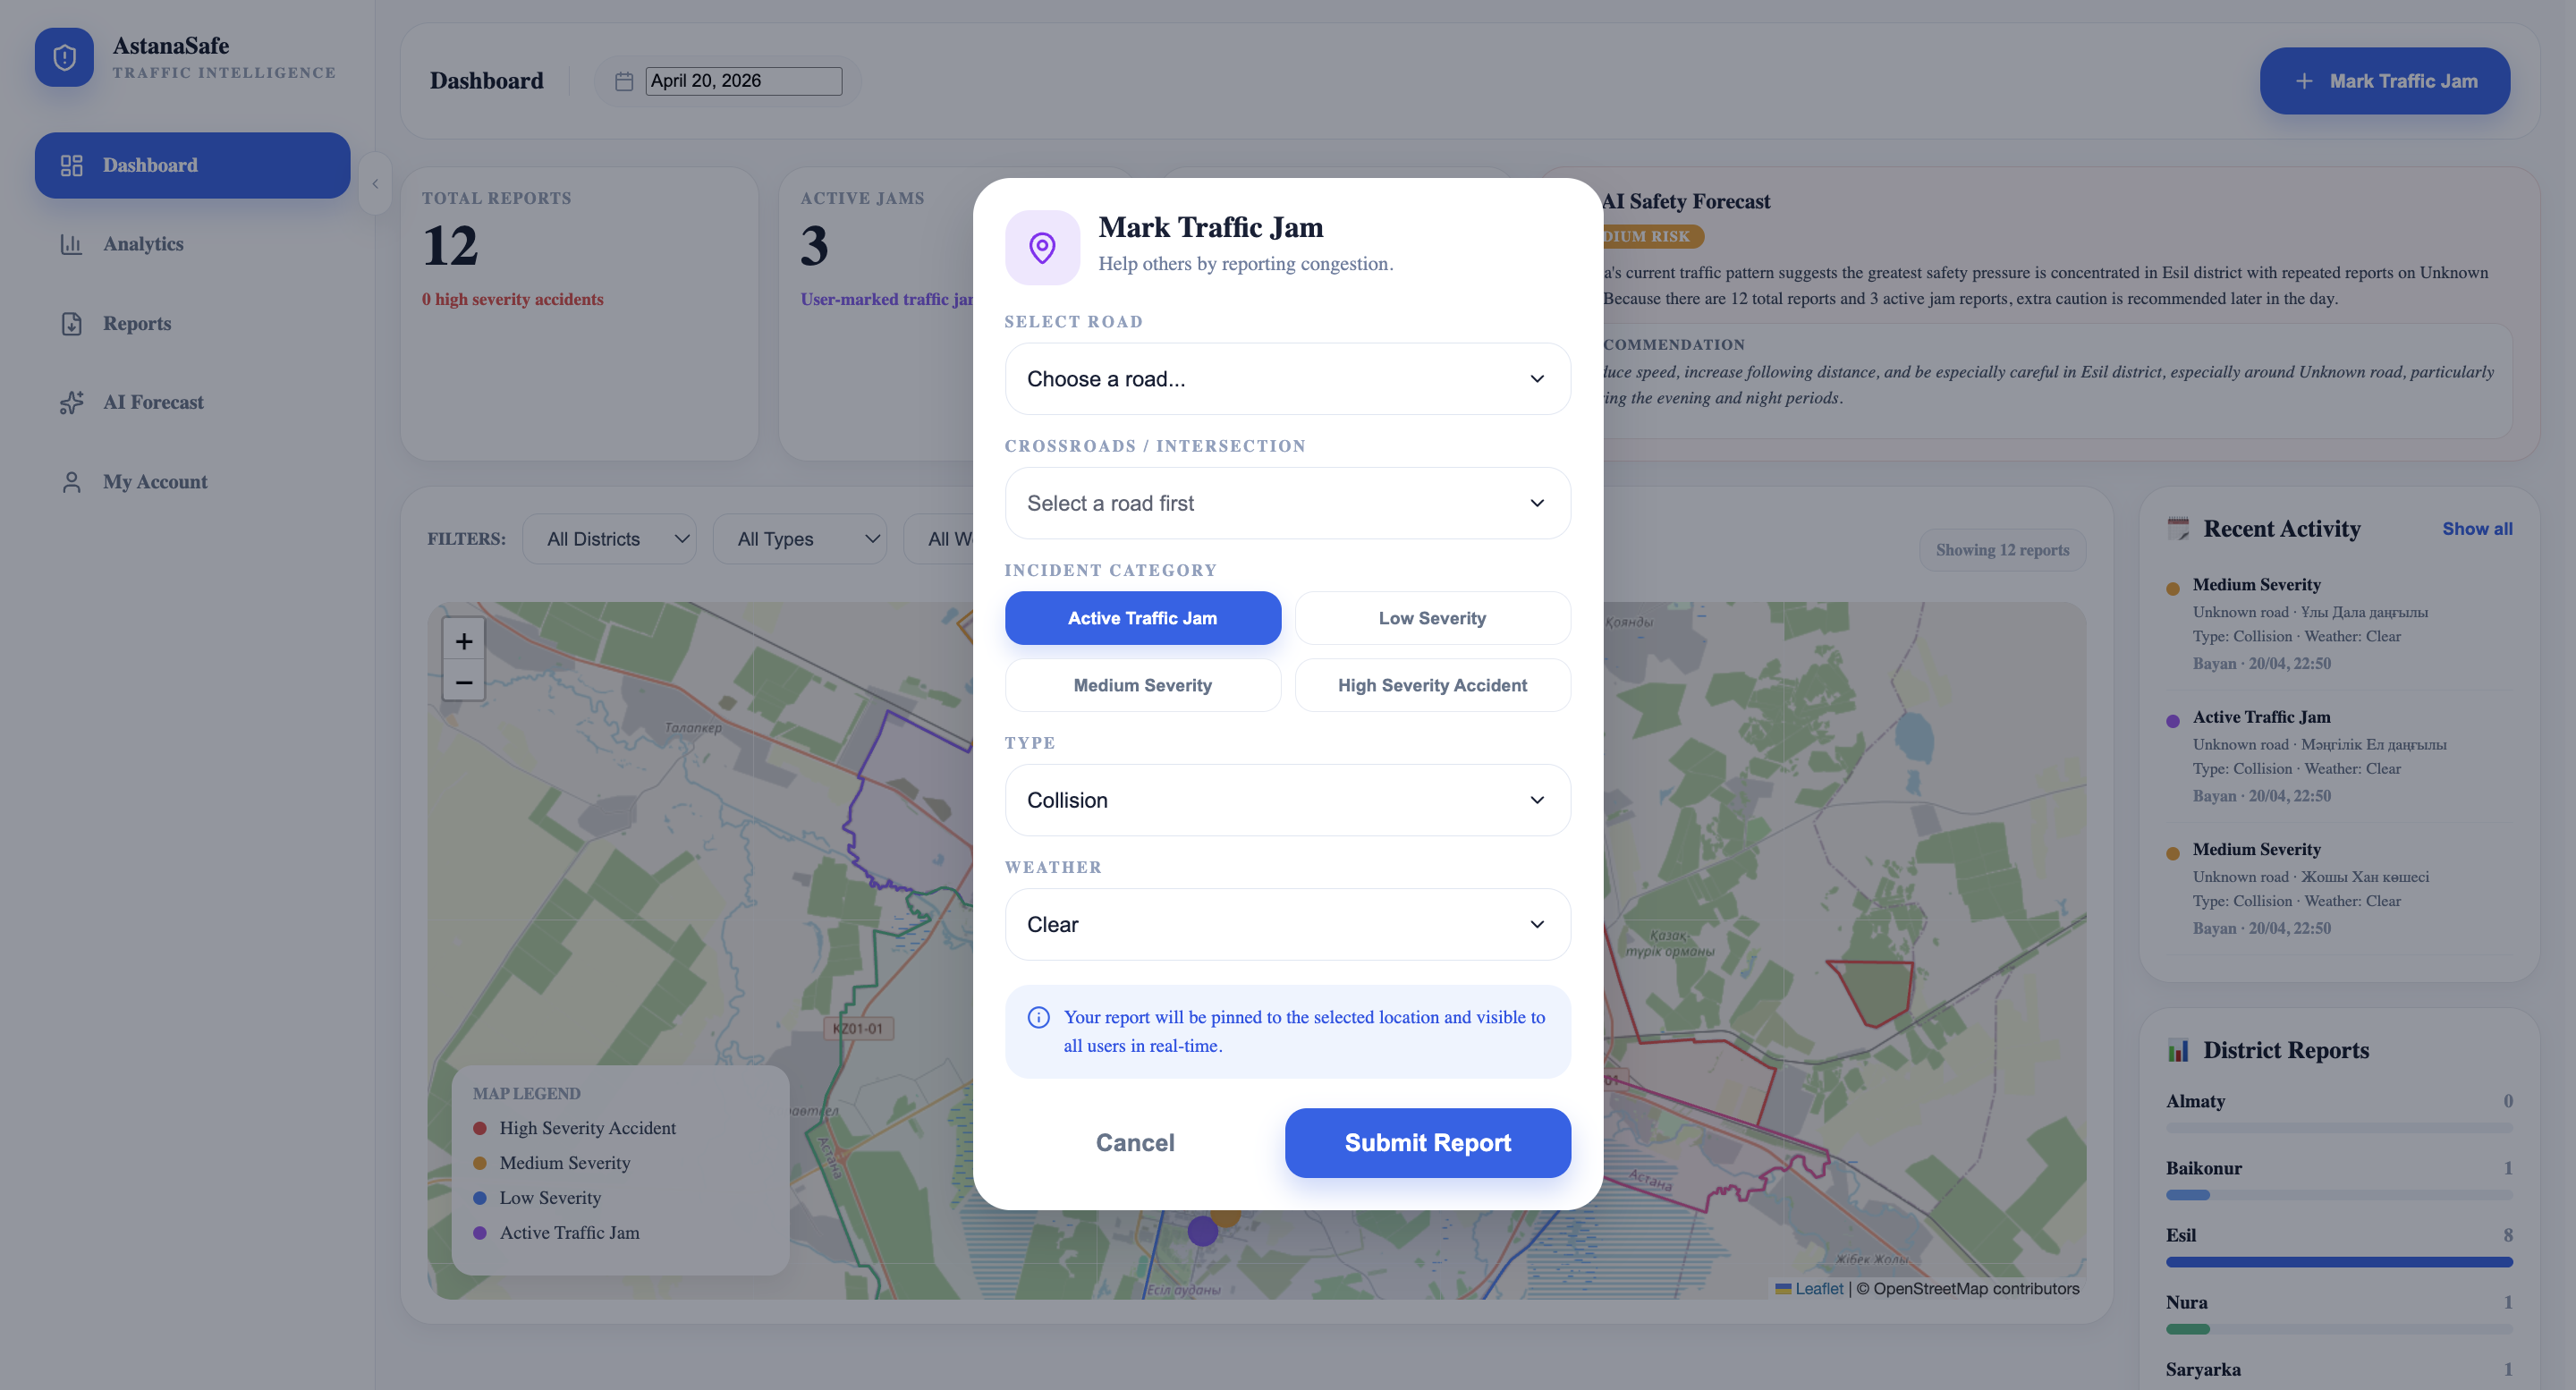
\includegraphics[width=0.82\textwidth]{sc2_mark_jam}
  \caption{\centering Mark Traffic Jam modal form, showing the road selector,
           crossroads dropdown, incident category selector
           (Active Traffic Jam, Low / Medium / High Severity), type and weather
           dropdowns, and the real-time visibility notification.}
  \label{fig:app_mark_jam}
\end{figure}

\begin{figure}[H]
  \centering
  \addcontentsline{toc}{subsection}{Figure 8}
  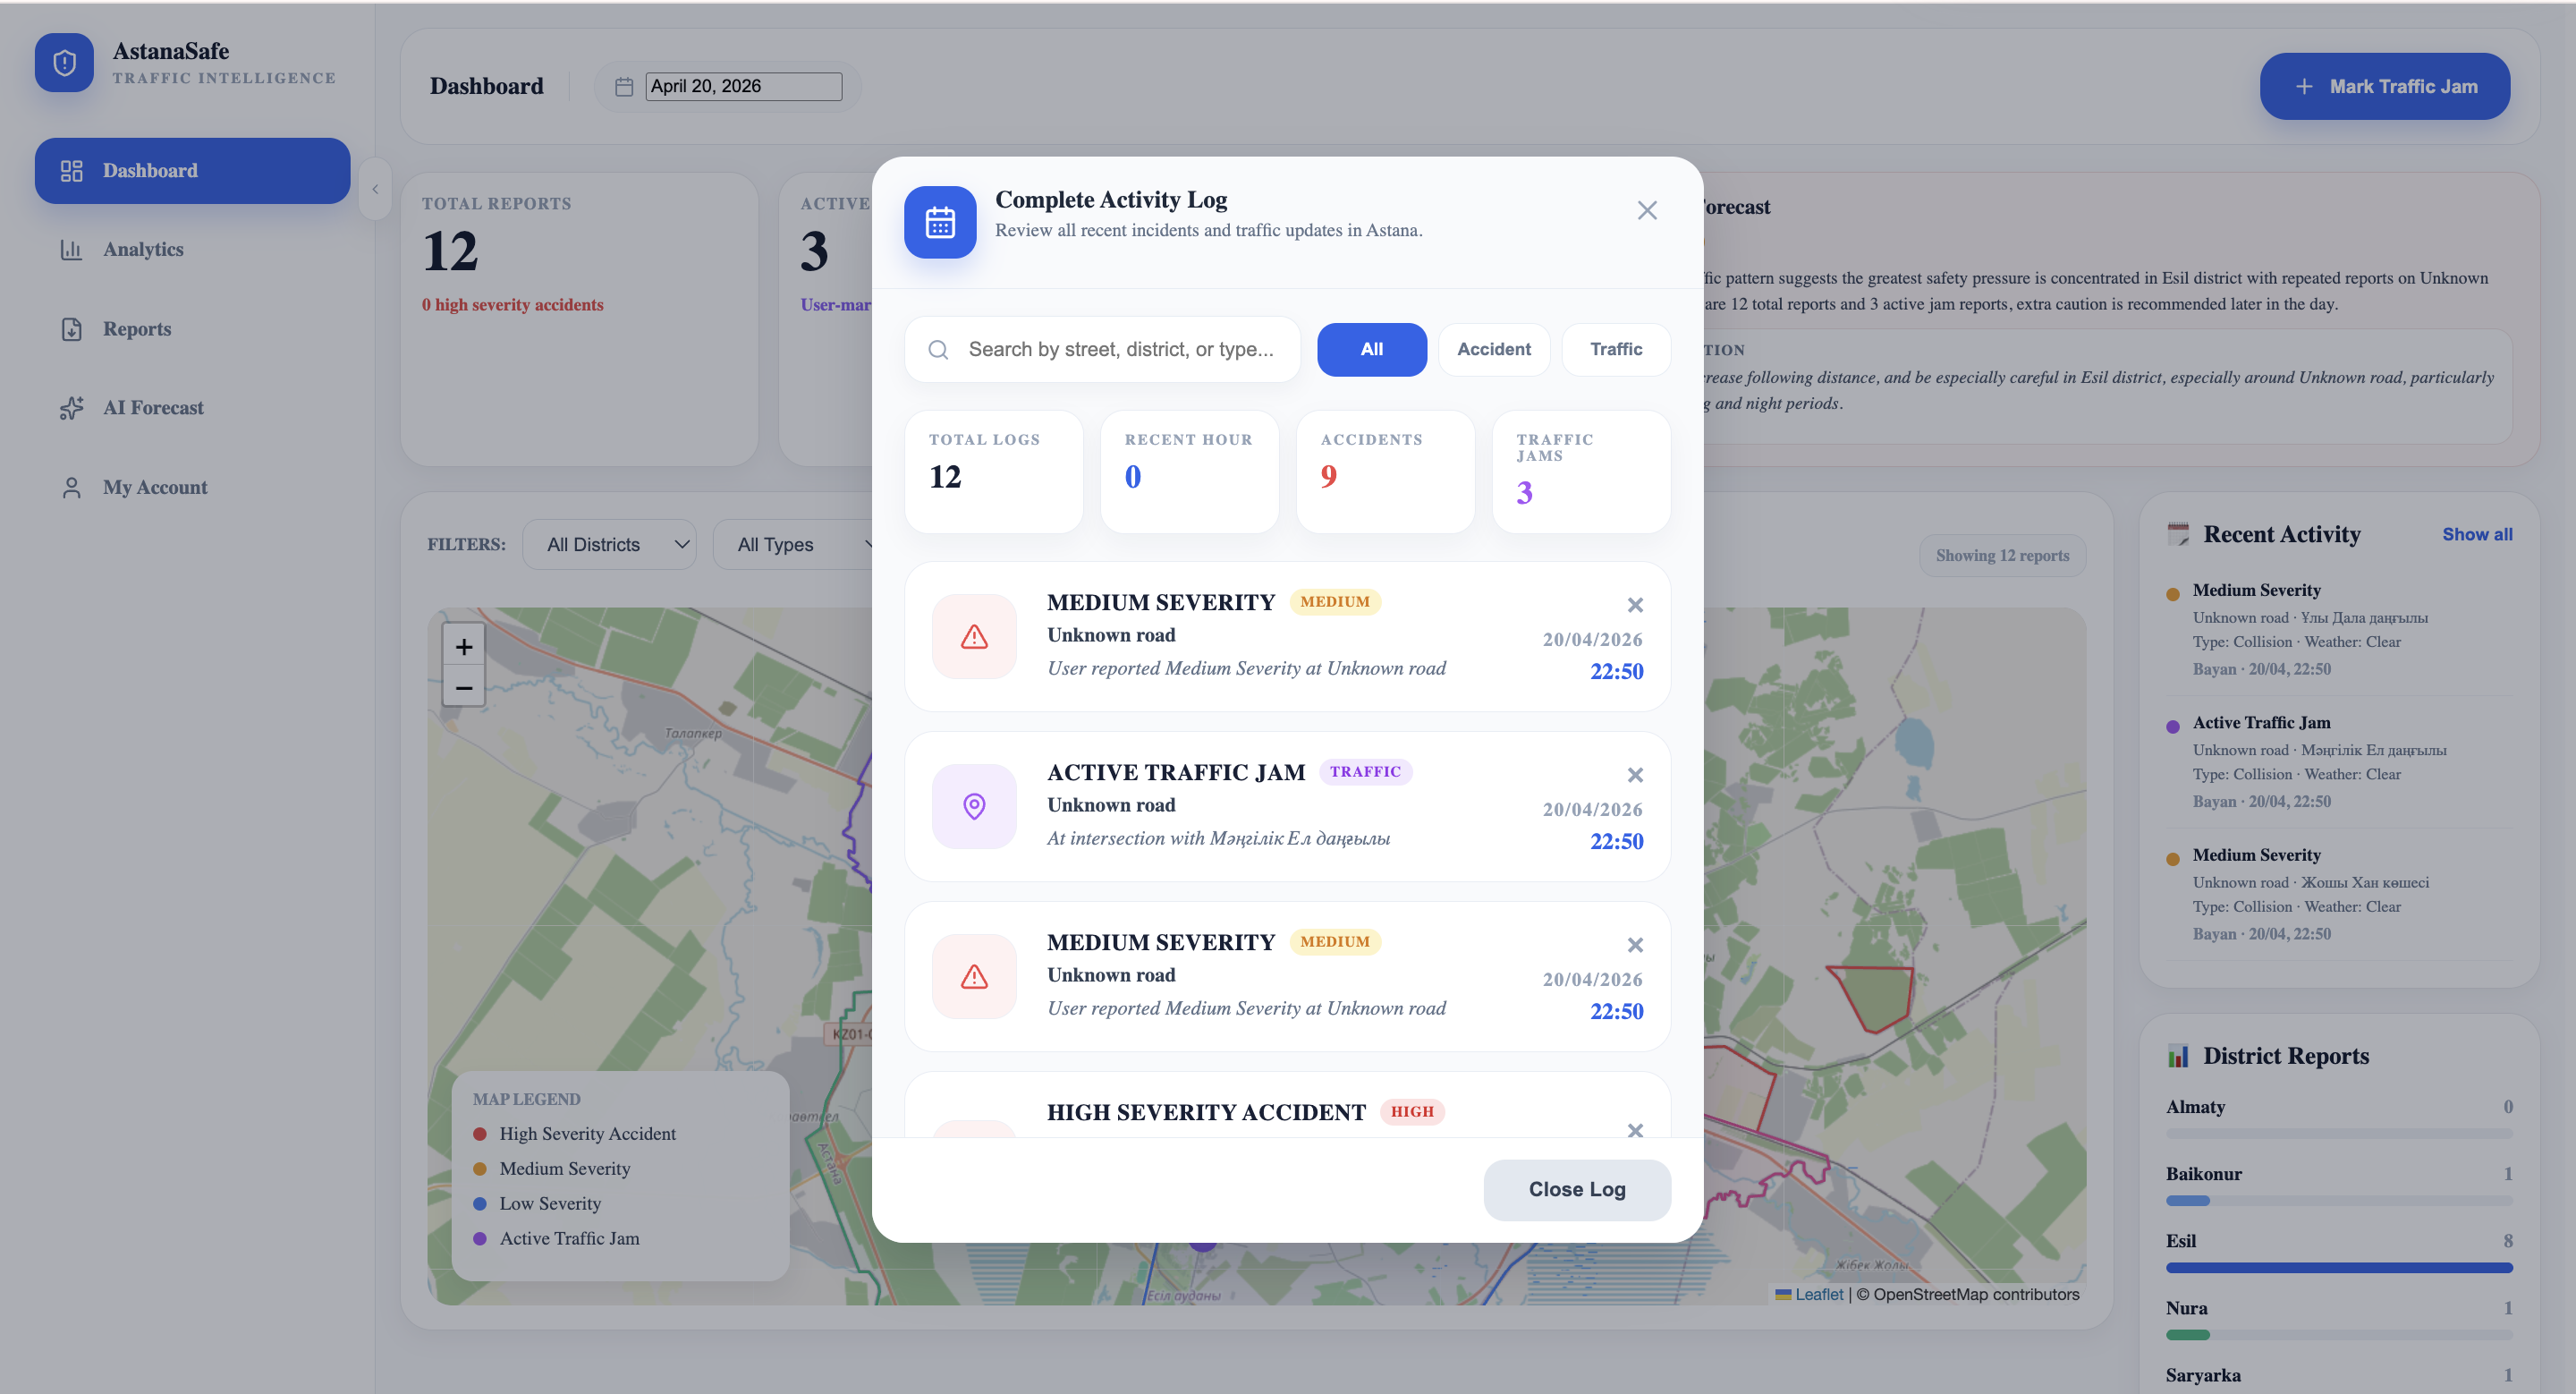
\includegraphics[width=0.82\textwidth]{sc3_activity_log}
  \caption{\centering Complete Activity Log modal displaying 12 total logs
           (9 accidents, 3 traffic jams) for the selected date, with search field,
           type filter tabs, and per-entry severity badges, road names,
           and deletion controls.}
  \label{fig:app_activity_log}
\end{figure}

\begin{figure}[H]
  \centering
  \addcontentsline{toc}{subsection}{Figure 9}
  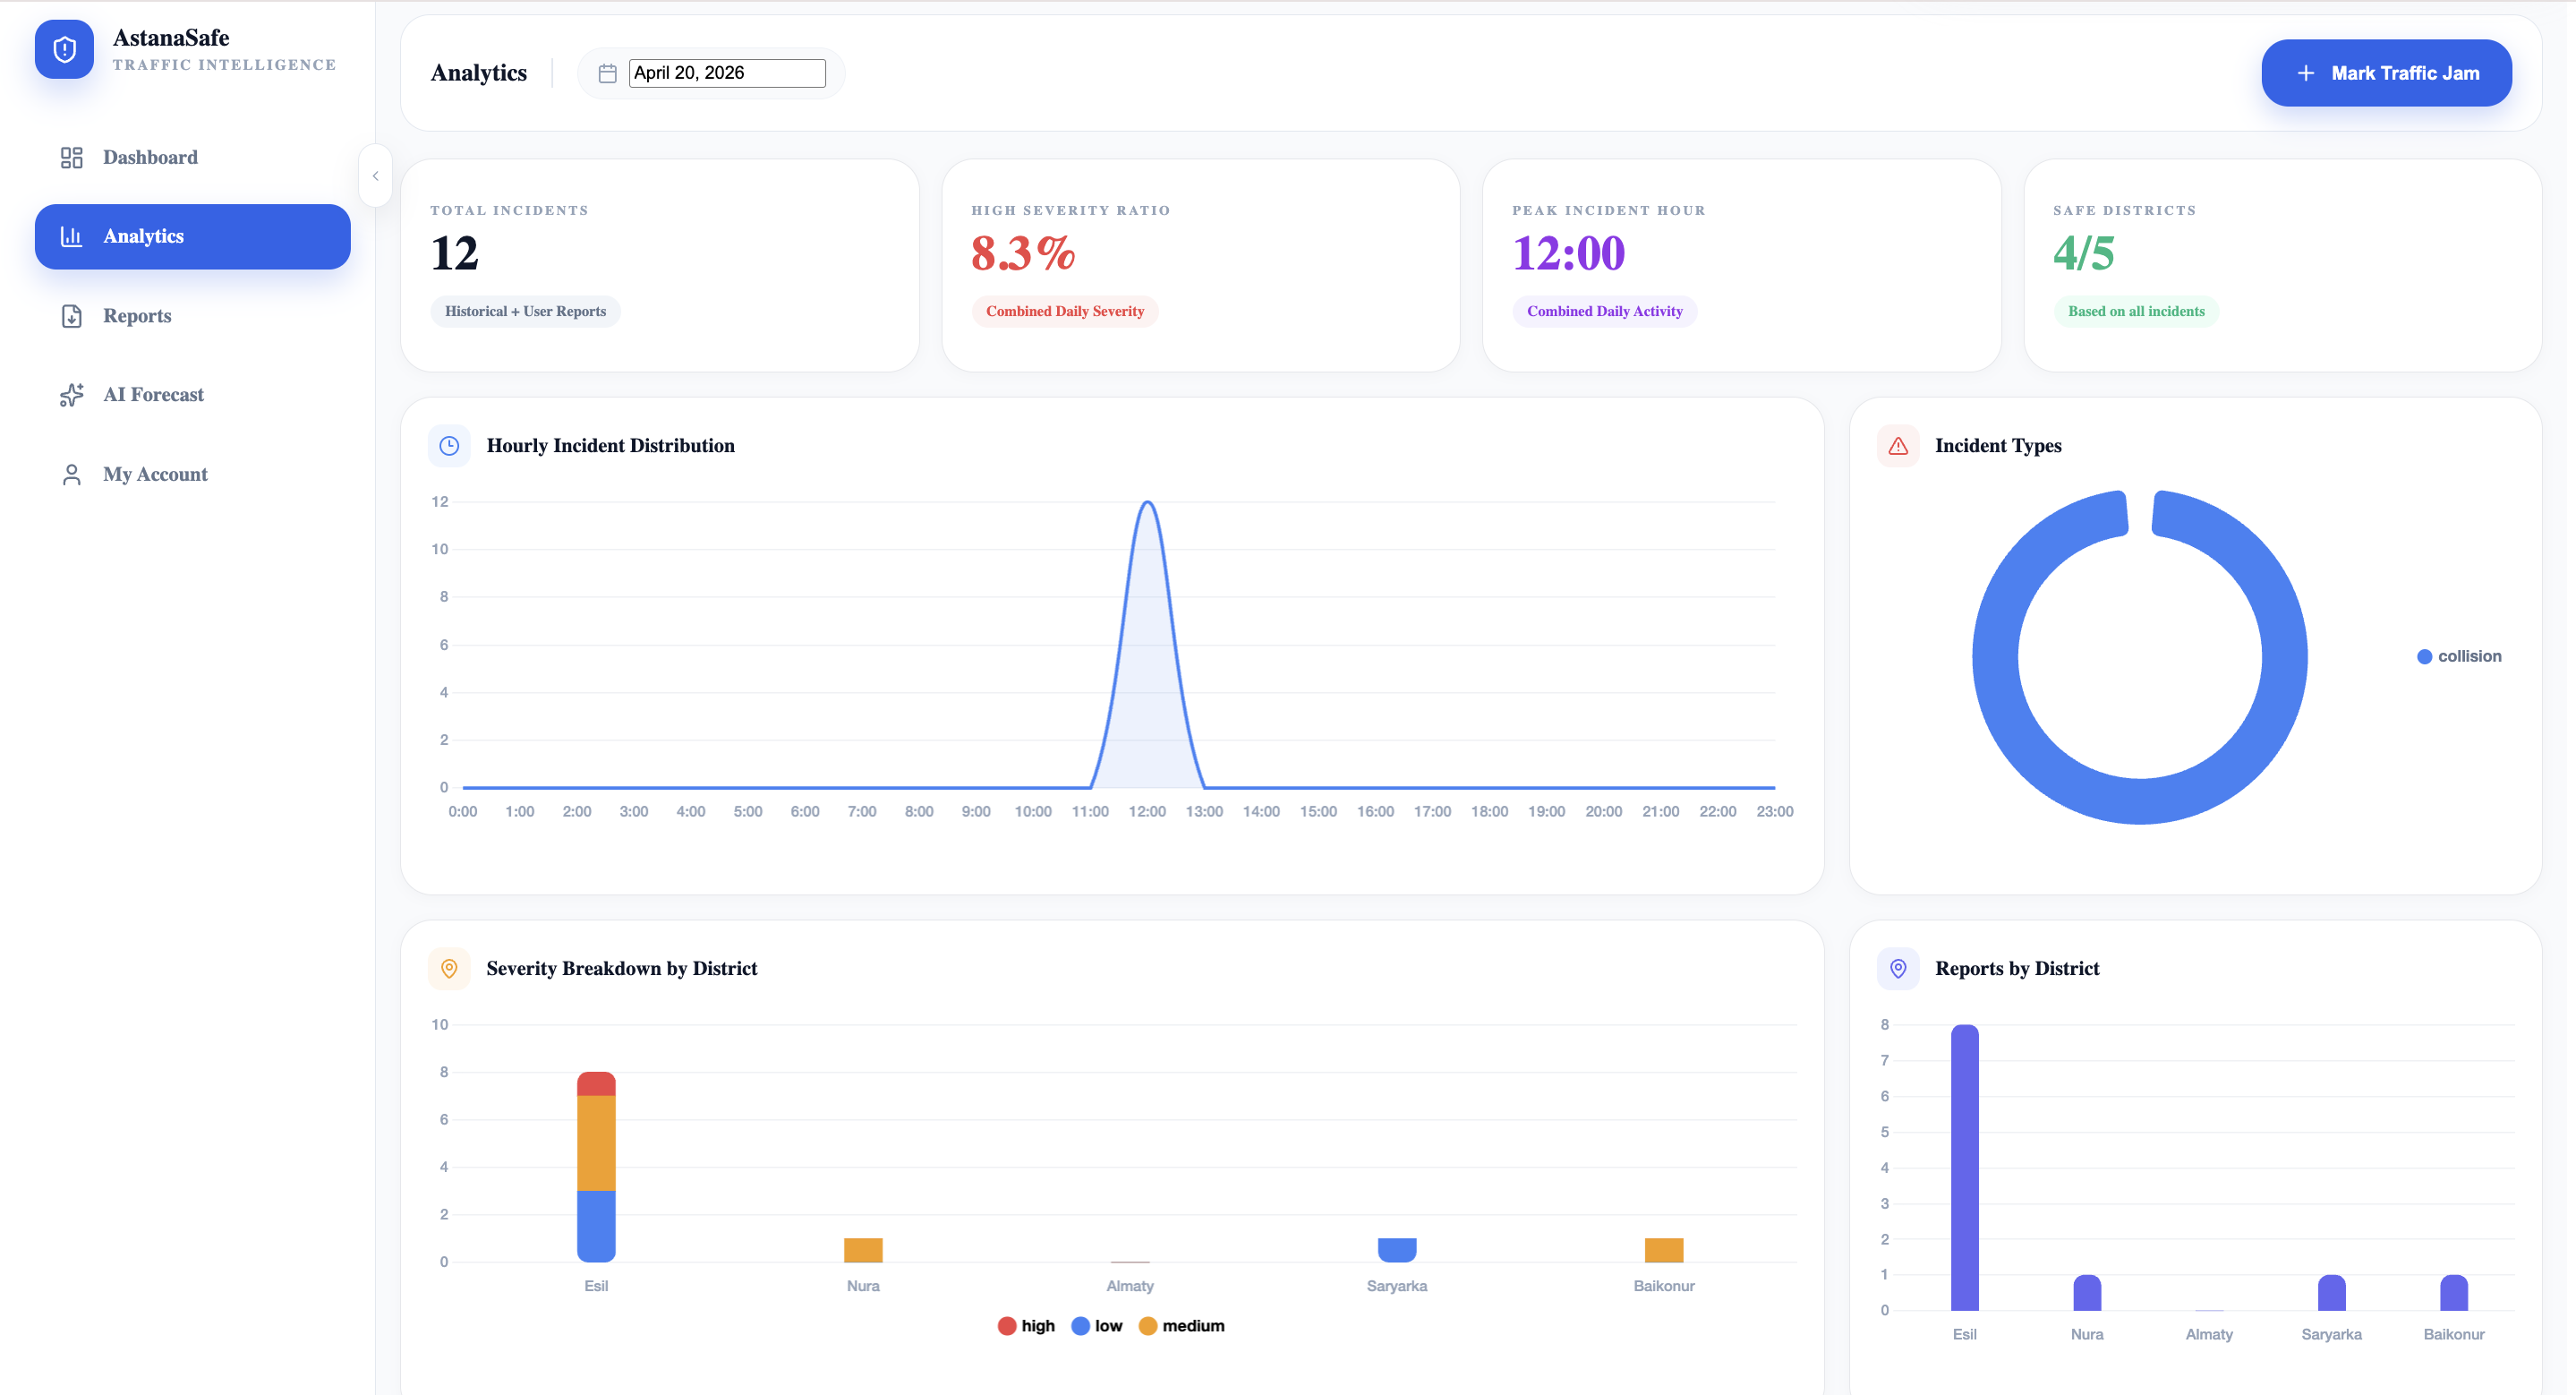
\includegraphics[width=\textwidth]{sc4_analytics}
  \caption{\centering Analytics page (upper section): KPI summary cards
           (12 total incidents, 8.3\,\% high severity, peak hour 12:00,
           4/6 safe districts), hourly incident distribution line chart,
           and incident types donut chart.}
  \label{fig:app_analytics}
\end{figure}

\begin{figure}[H]
  \centering
  \addcontentsline{toc}{subsection}{Figure 10}
  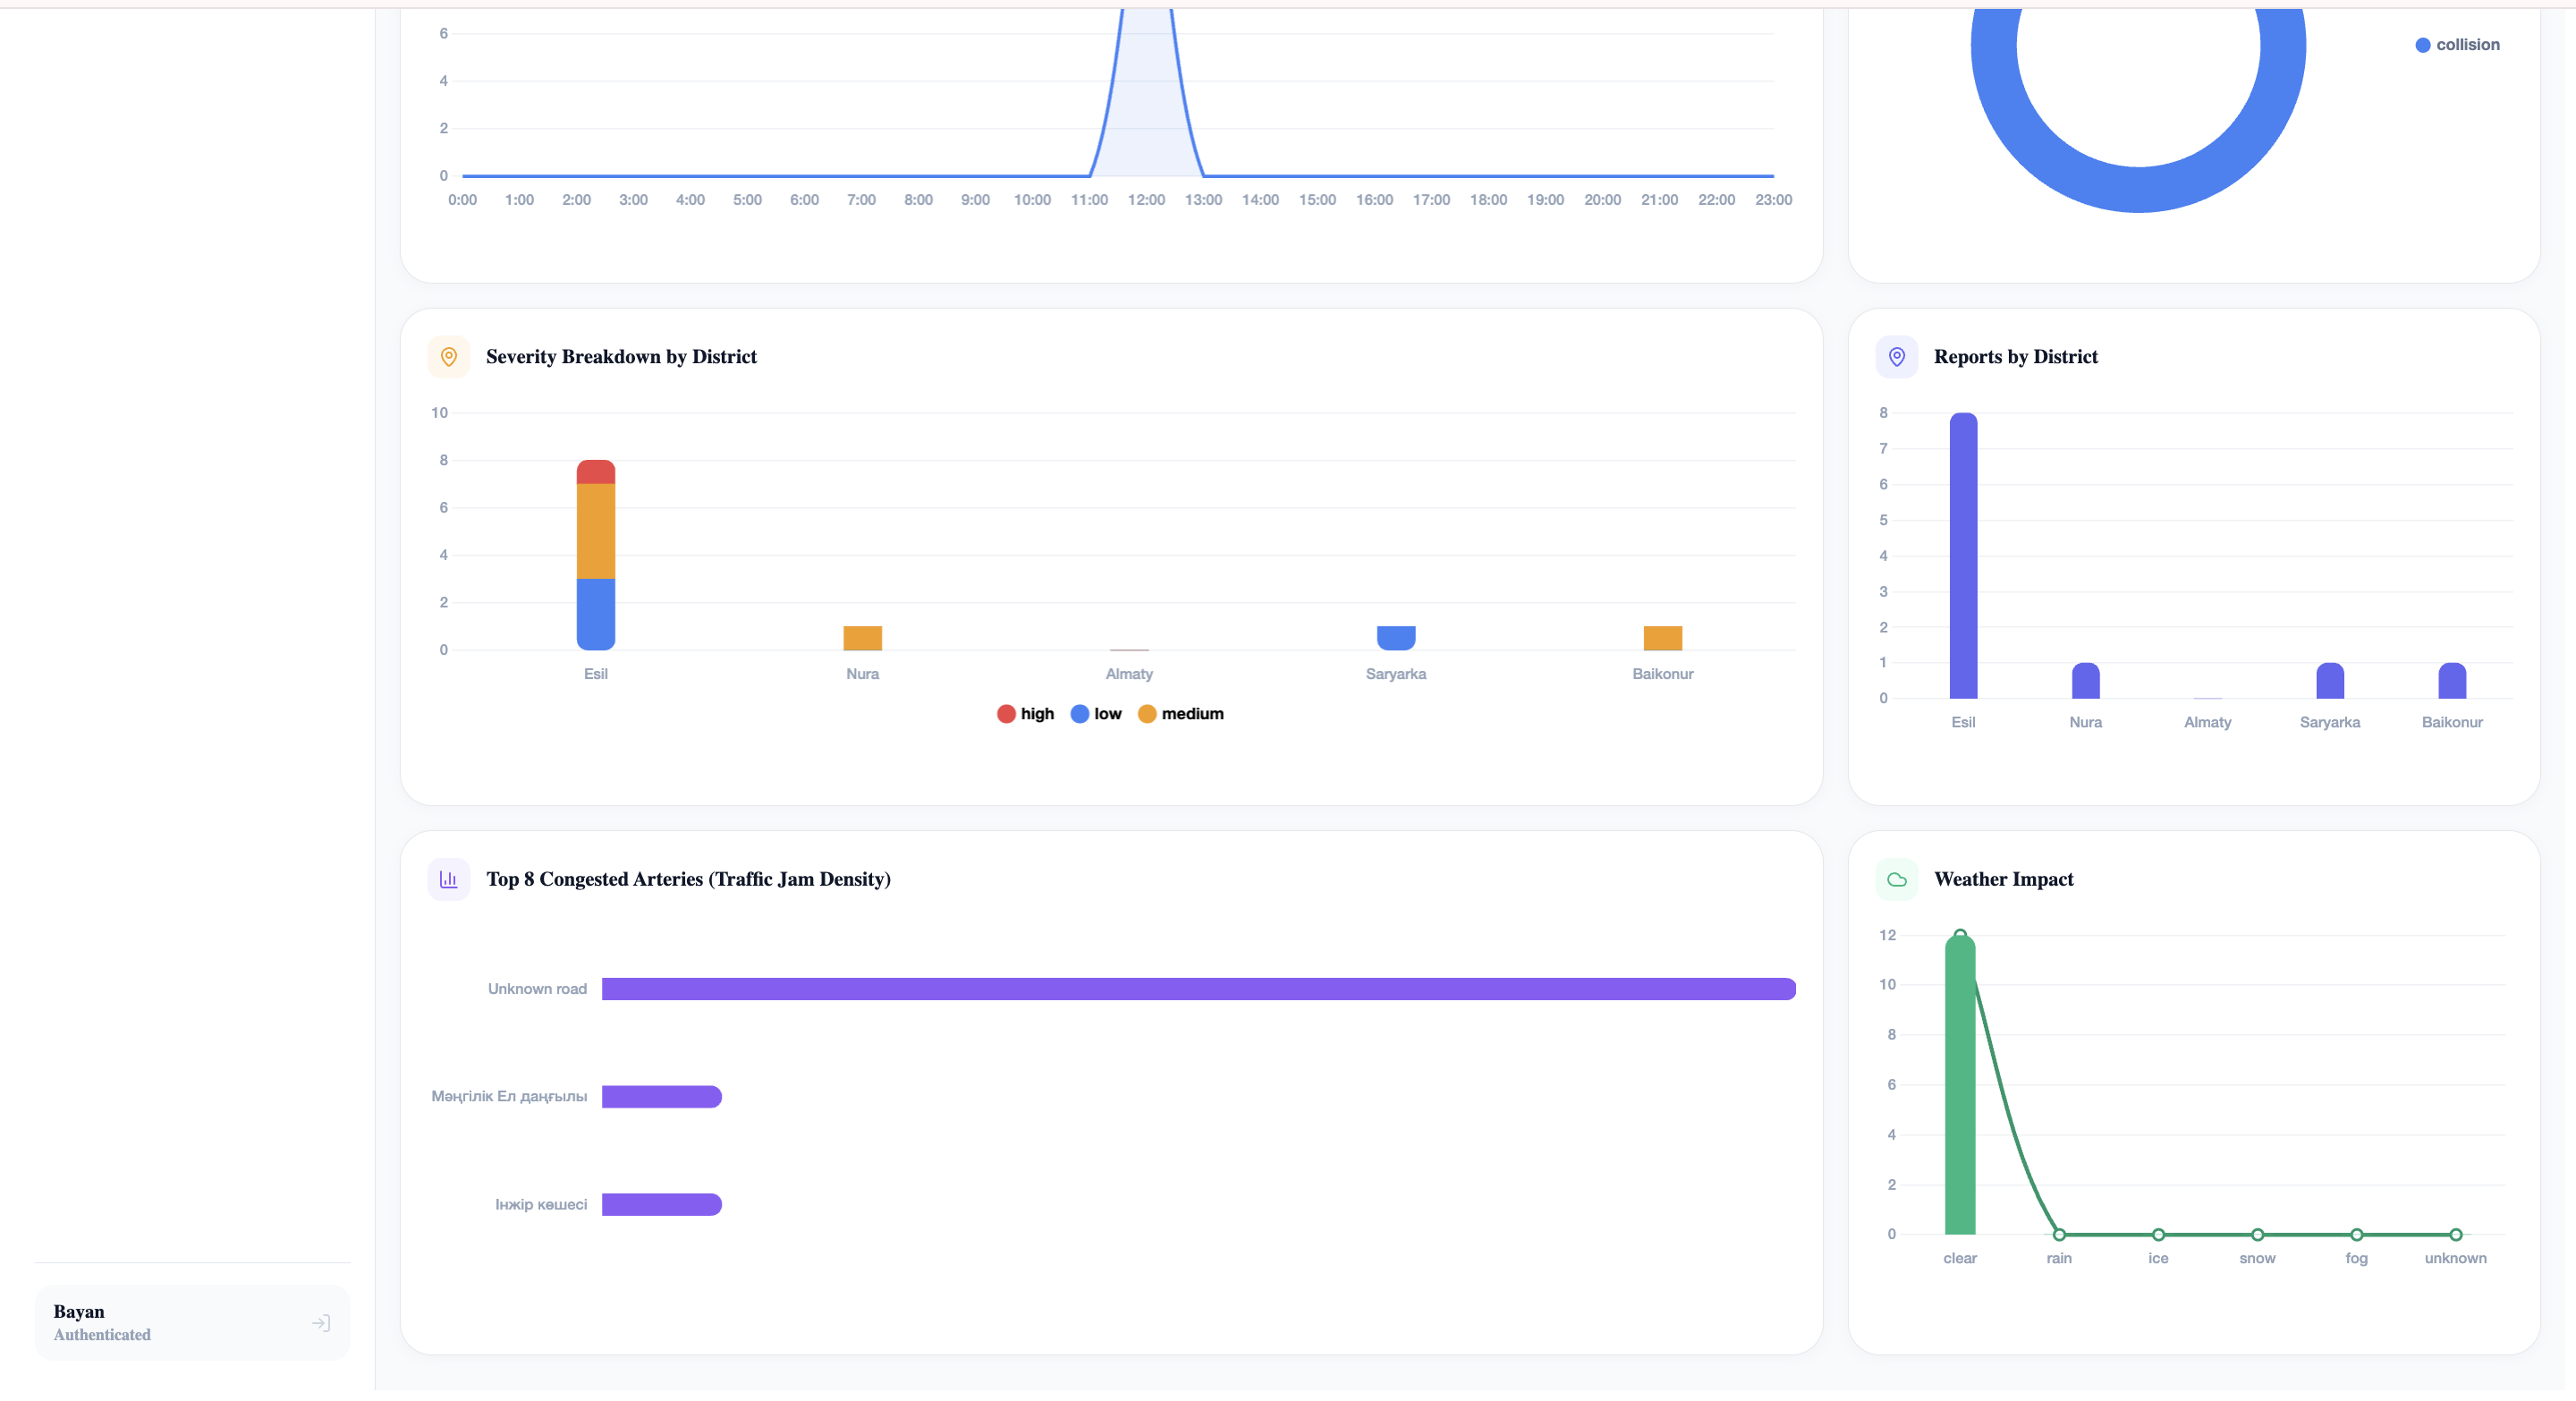
\includegraphics[width=\textwidth]{sc5_analytics2}
  \caption{\centering Analytics page (lower section): severity breakdown by
           district stacked bar chart, reports by district bar chart,
           top~8 congested arteries horizontal bar ranking, and weather impact
           bar-and-line combination chart.}
  \label{fig:app_analytics2}
\end{figure}

\begin{figure}[H]
  \centering
  \addcontentsline{toc}{subsection}{Figure 11}
  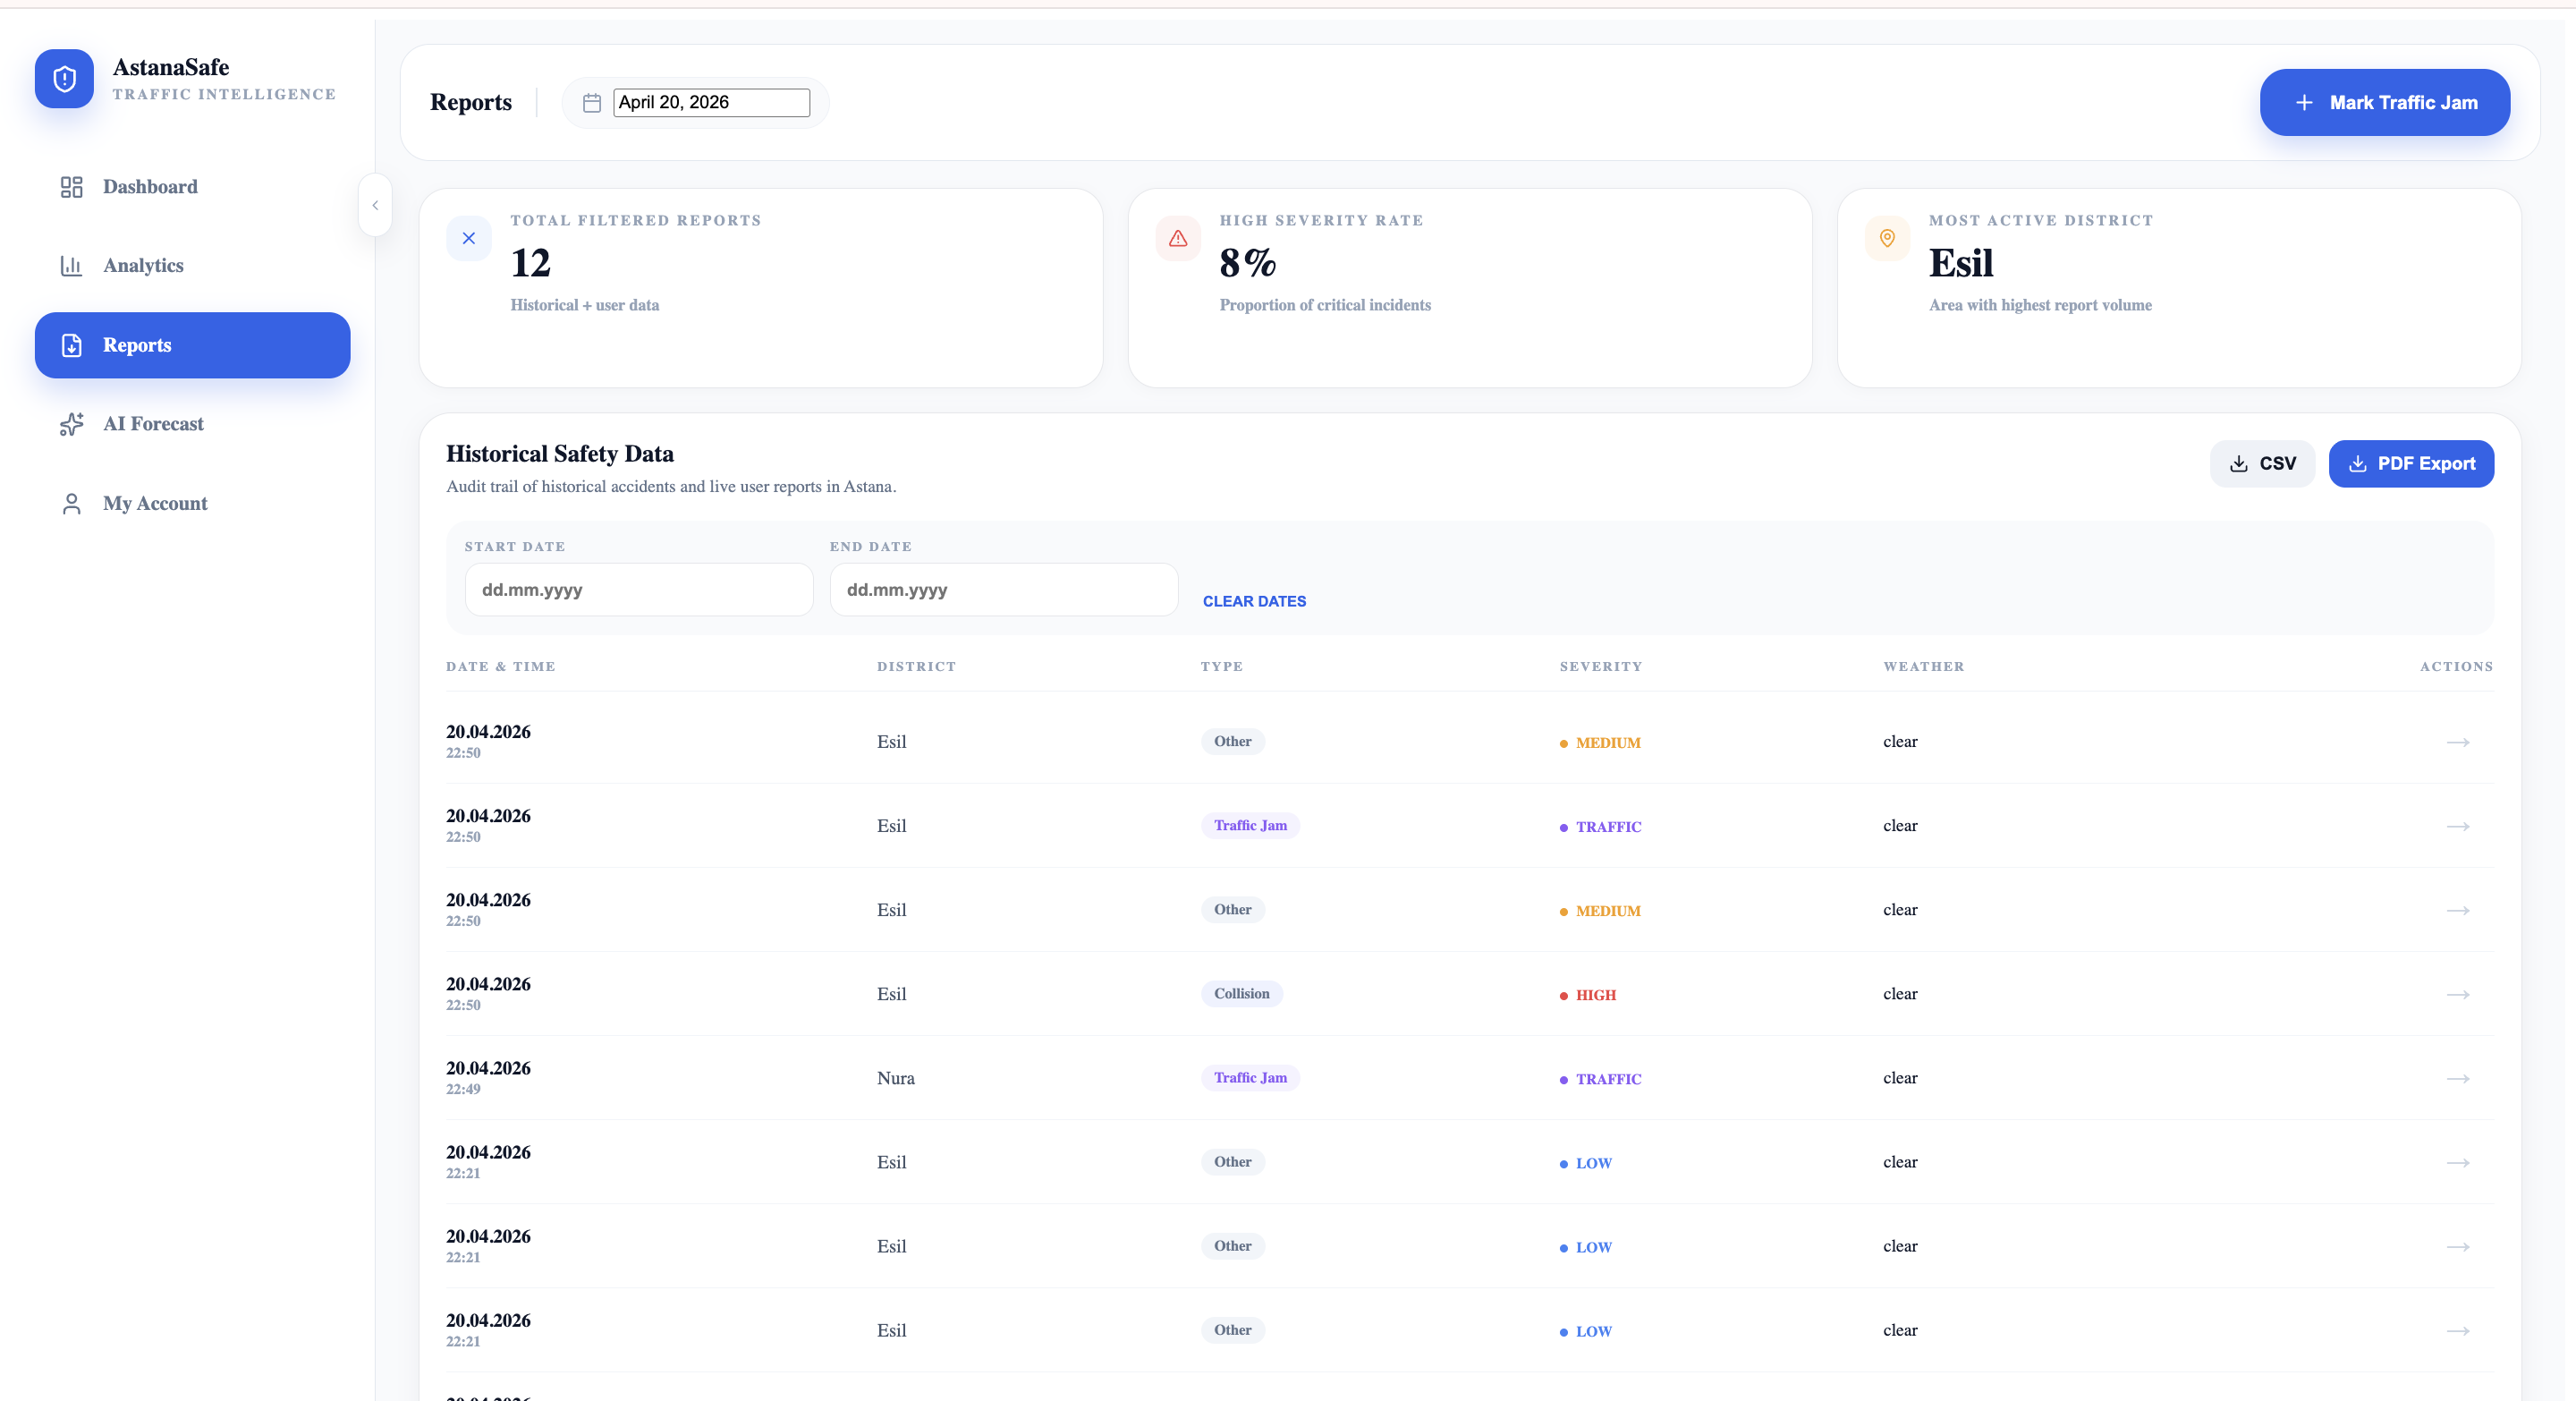
\includegraphics[width=\textwidth]{sc6_reports}
  \caption{\centering Reports page showing KPI cards (12 total reports,
           8\,\% high severity rate, Esil as most active district),
           date range filter panel with CSV and PDF export buttons,
           and the Historical Safety Data table with severity badges
           and View on Map action controls.}
  \label{fig:app_reports}
\end{figure}

\begin{figure}[H]
  \centering
  \addcontentsline{toc}{subsection}{Figure 12}
  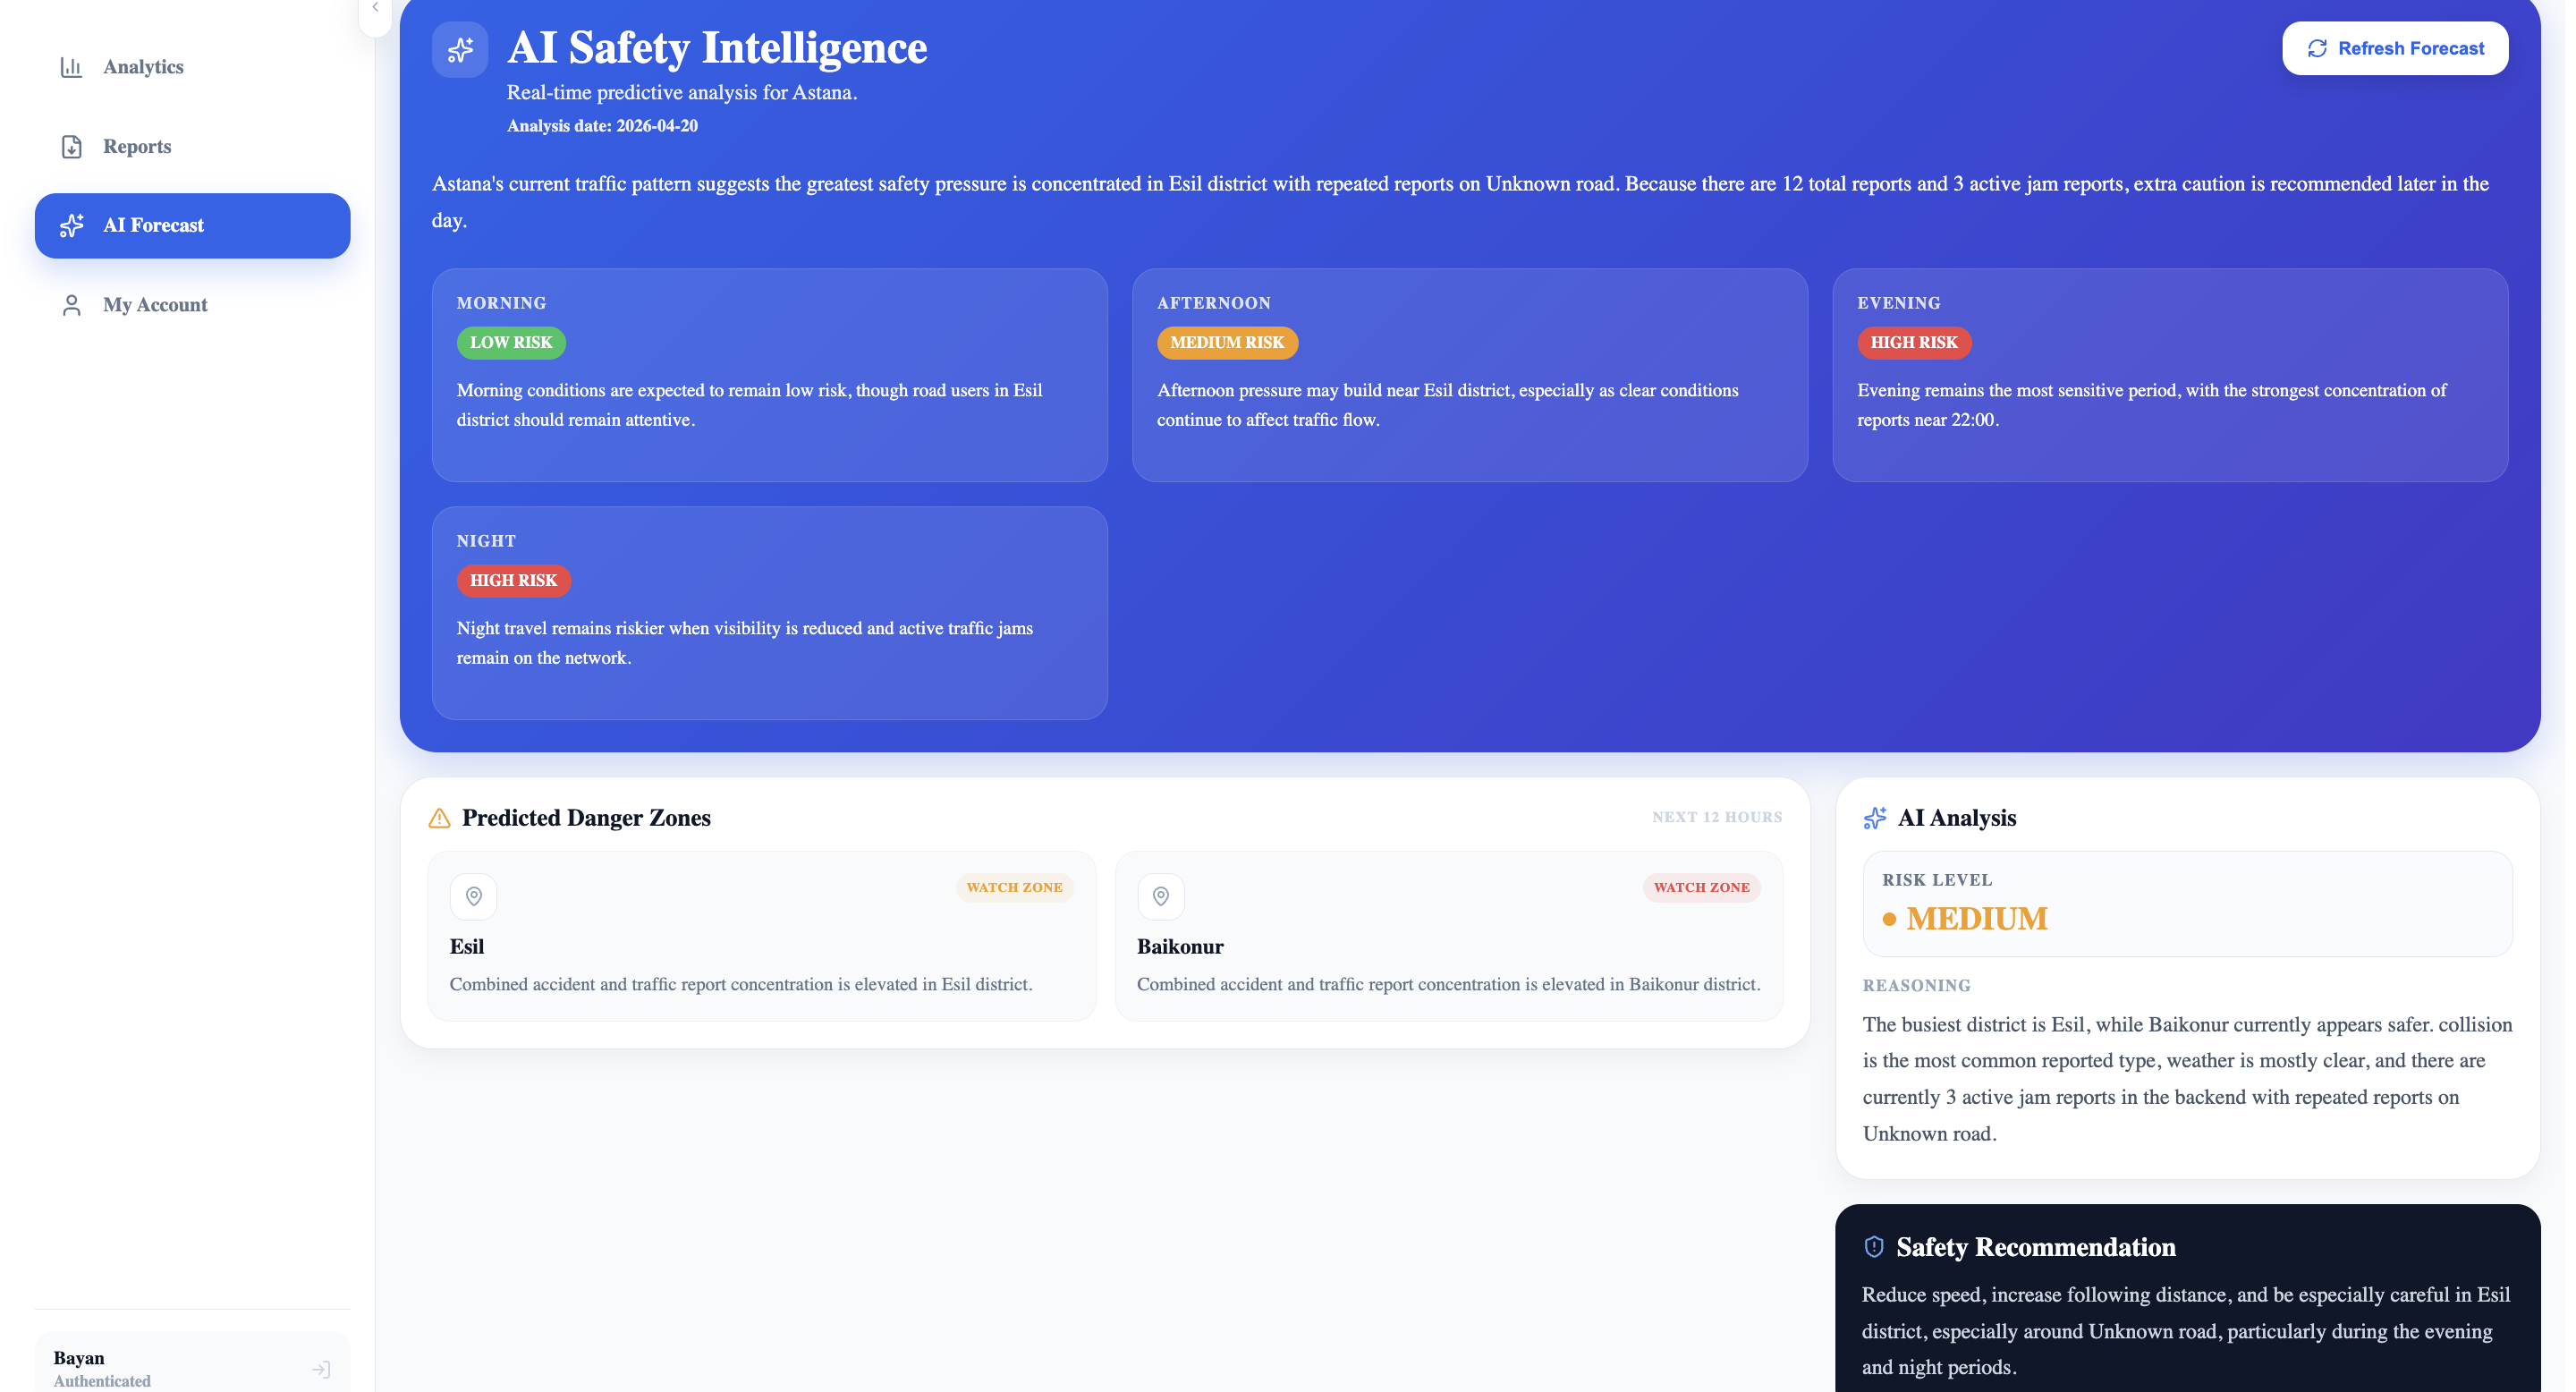
\includegraphics[width=\textwidth]{sc7_forecast}
  \caption{\centering AI Forecast page displaying four time-of-day risk cards
           (Morning: LOW, Afternoon: MEDIUM, Evening: HIGH, Night: HIGH),
           the Predicted Danger Zones panel (Esil and Baikonur flagged),
           the AI Analysis panel (MEDIUM overall risk with reasoning),
           and the Safety Recommendation panel.}
  \label{fig:app_forecast}
\end{figure}

\begin{figure}[H]
  \centering
  \addcontentsline{toc}{subsection}{Figure 13}
  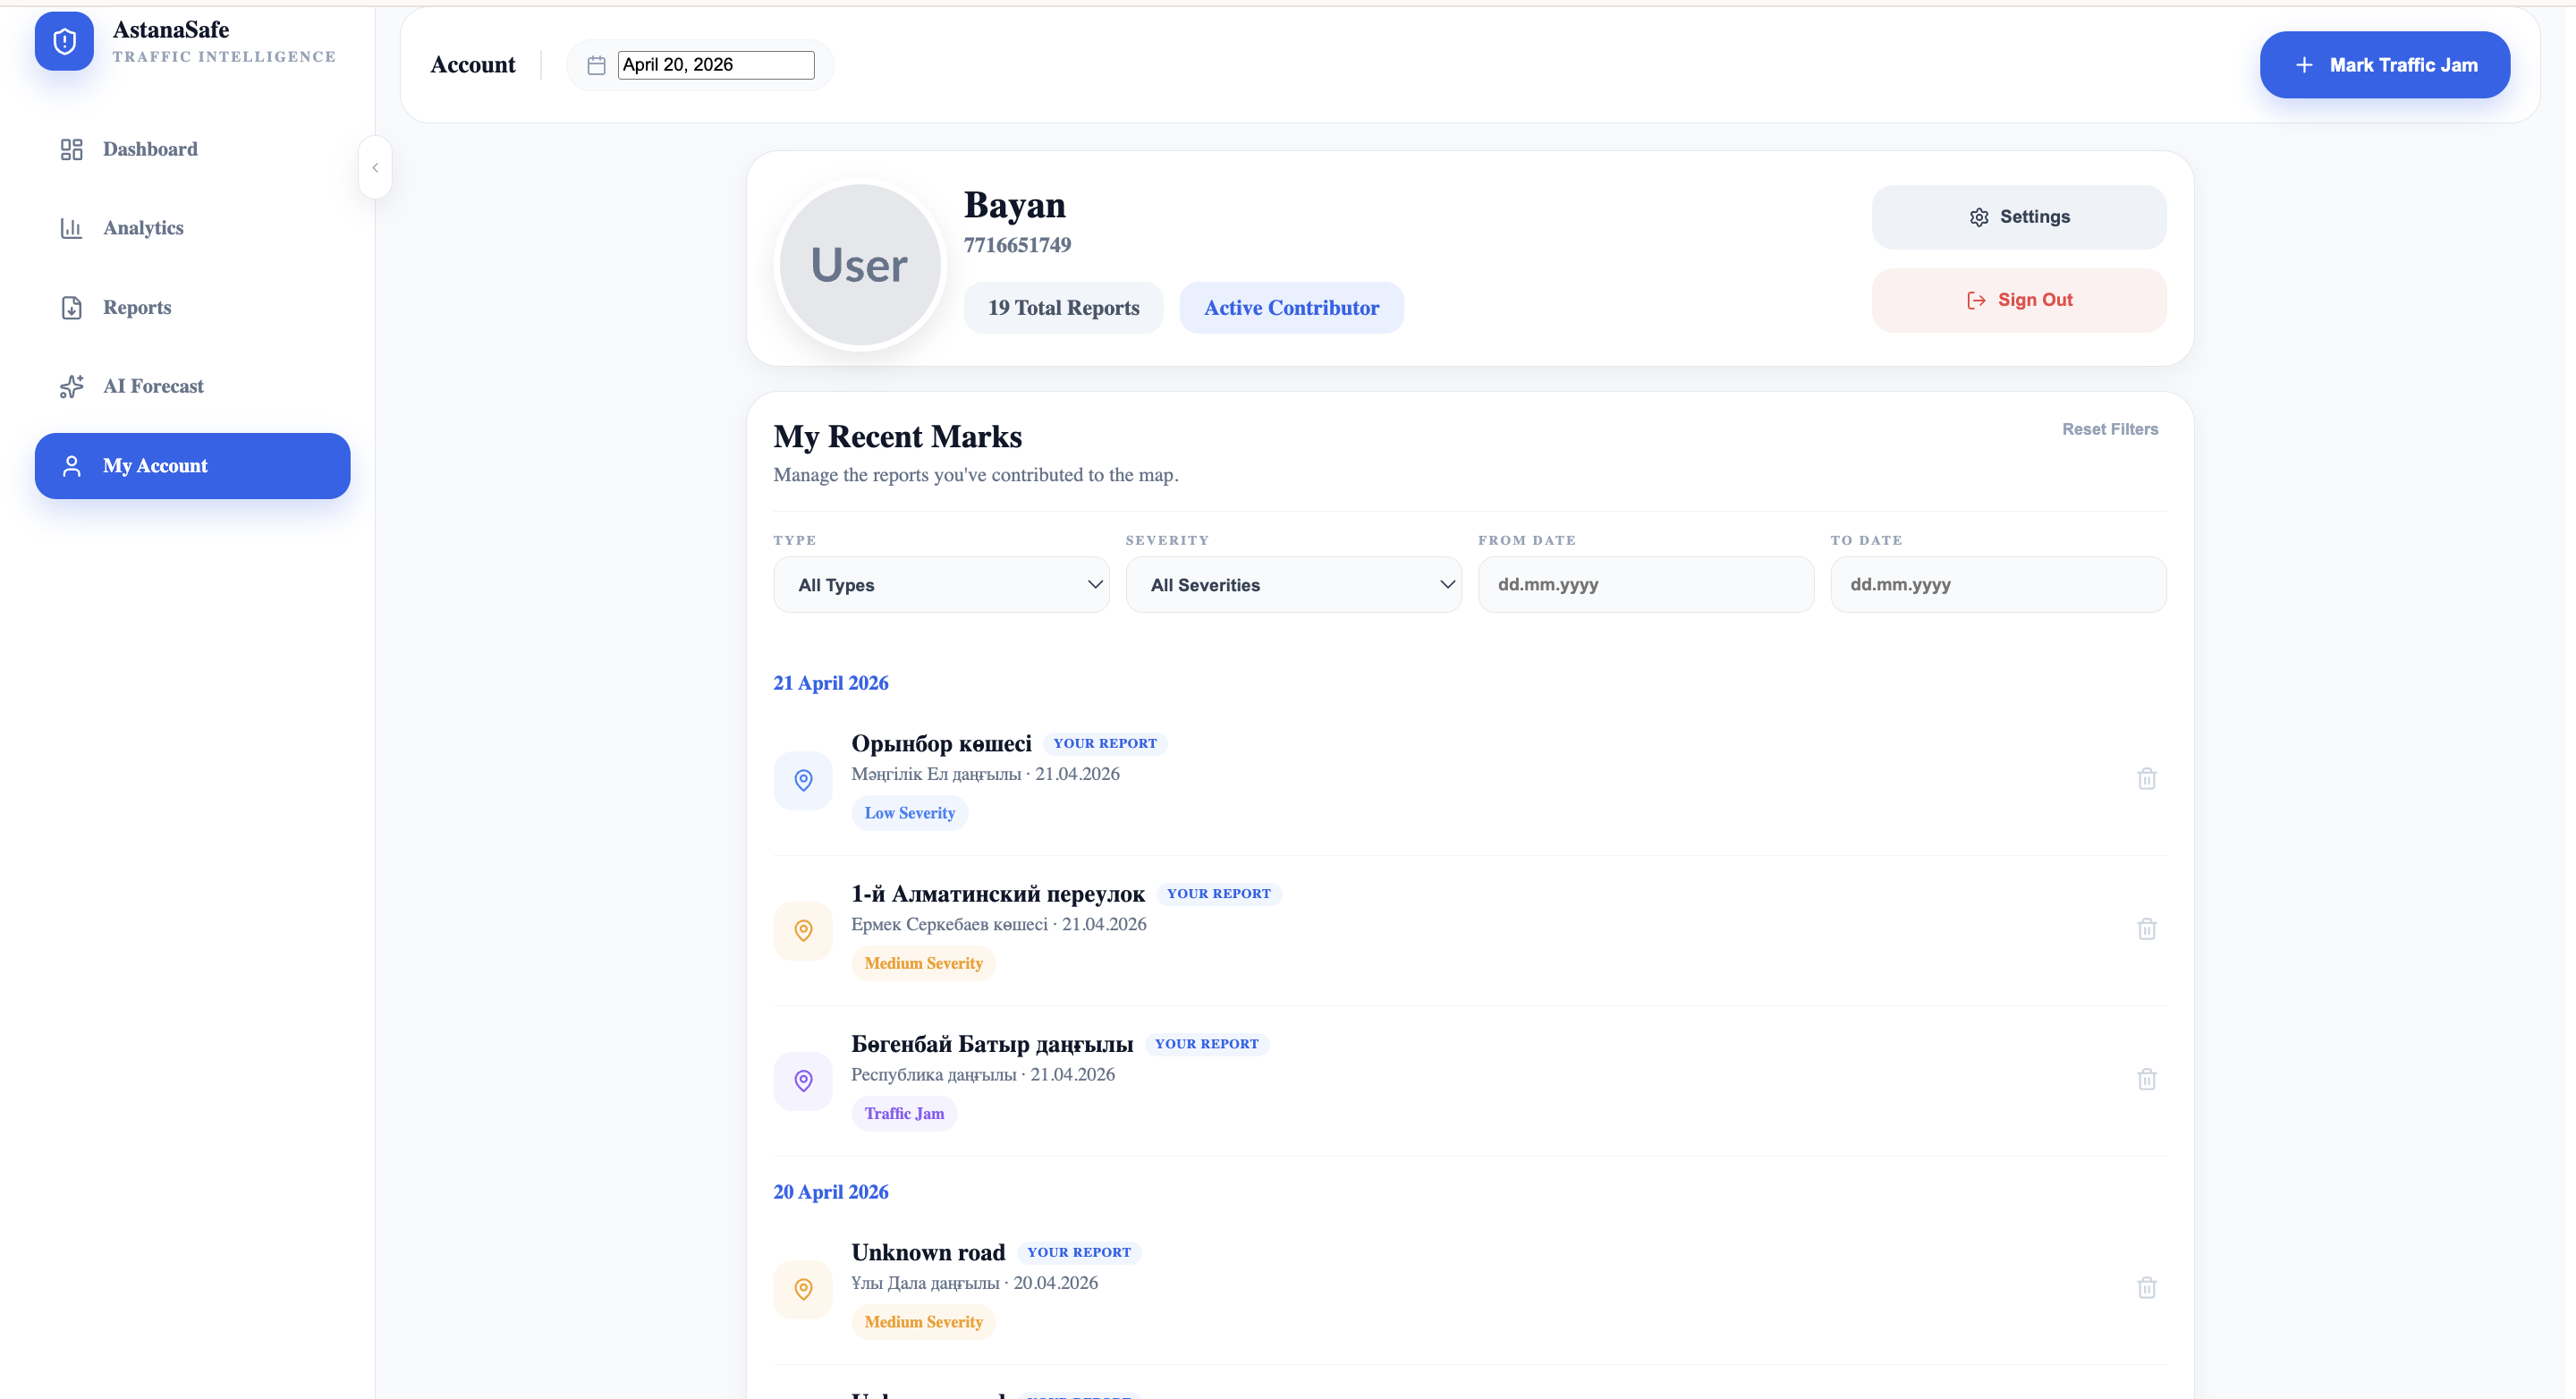
\includegraphics[width=\textwidth]{sc8_account}
  \caption{\centering Account page showing the user profile summary card
           (name, contact number, contribution badges), the My Recent Marks
           chronological submission list with severity labels, and the personal
           filter controls for type, severity, and date range.}
  \label{fig:app_account}
\end{figure}

\begin{figure}[H]
  \centering
  \addcontentsline{toc}{subsection}{Figure 14}
  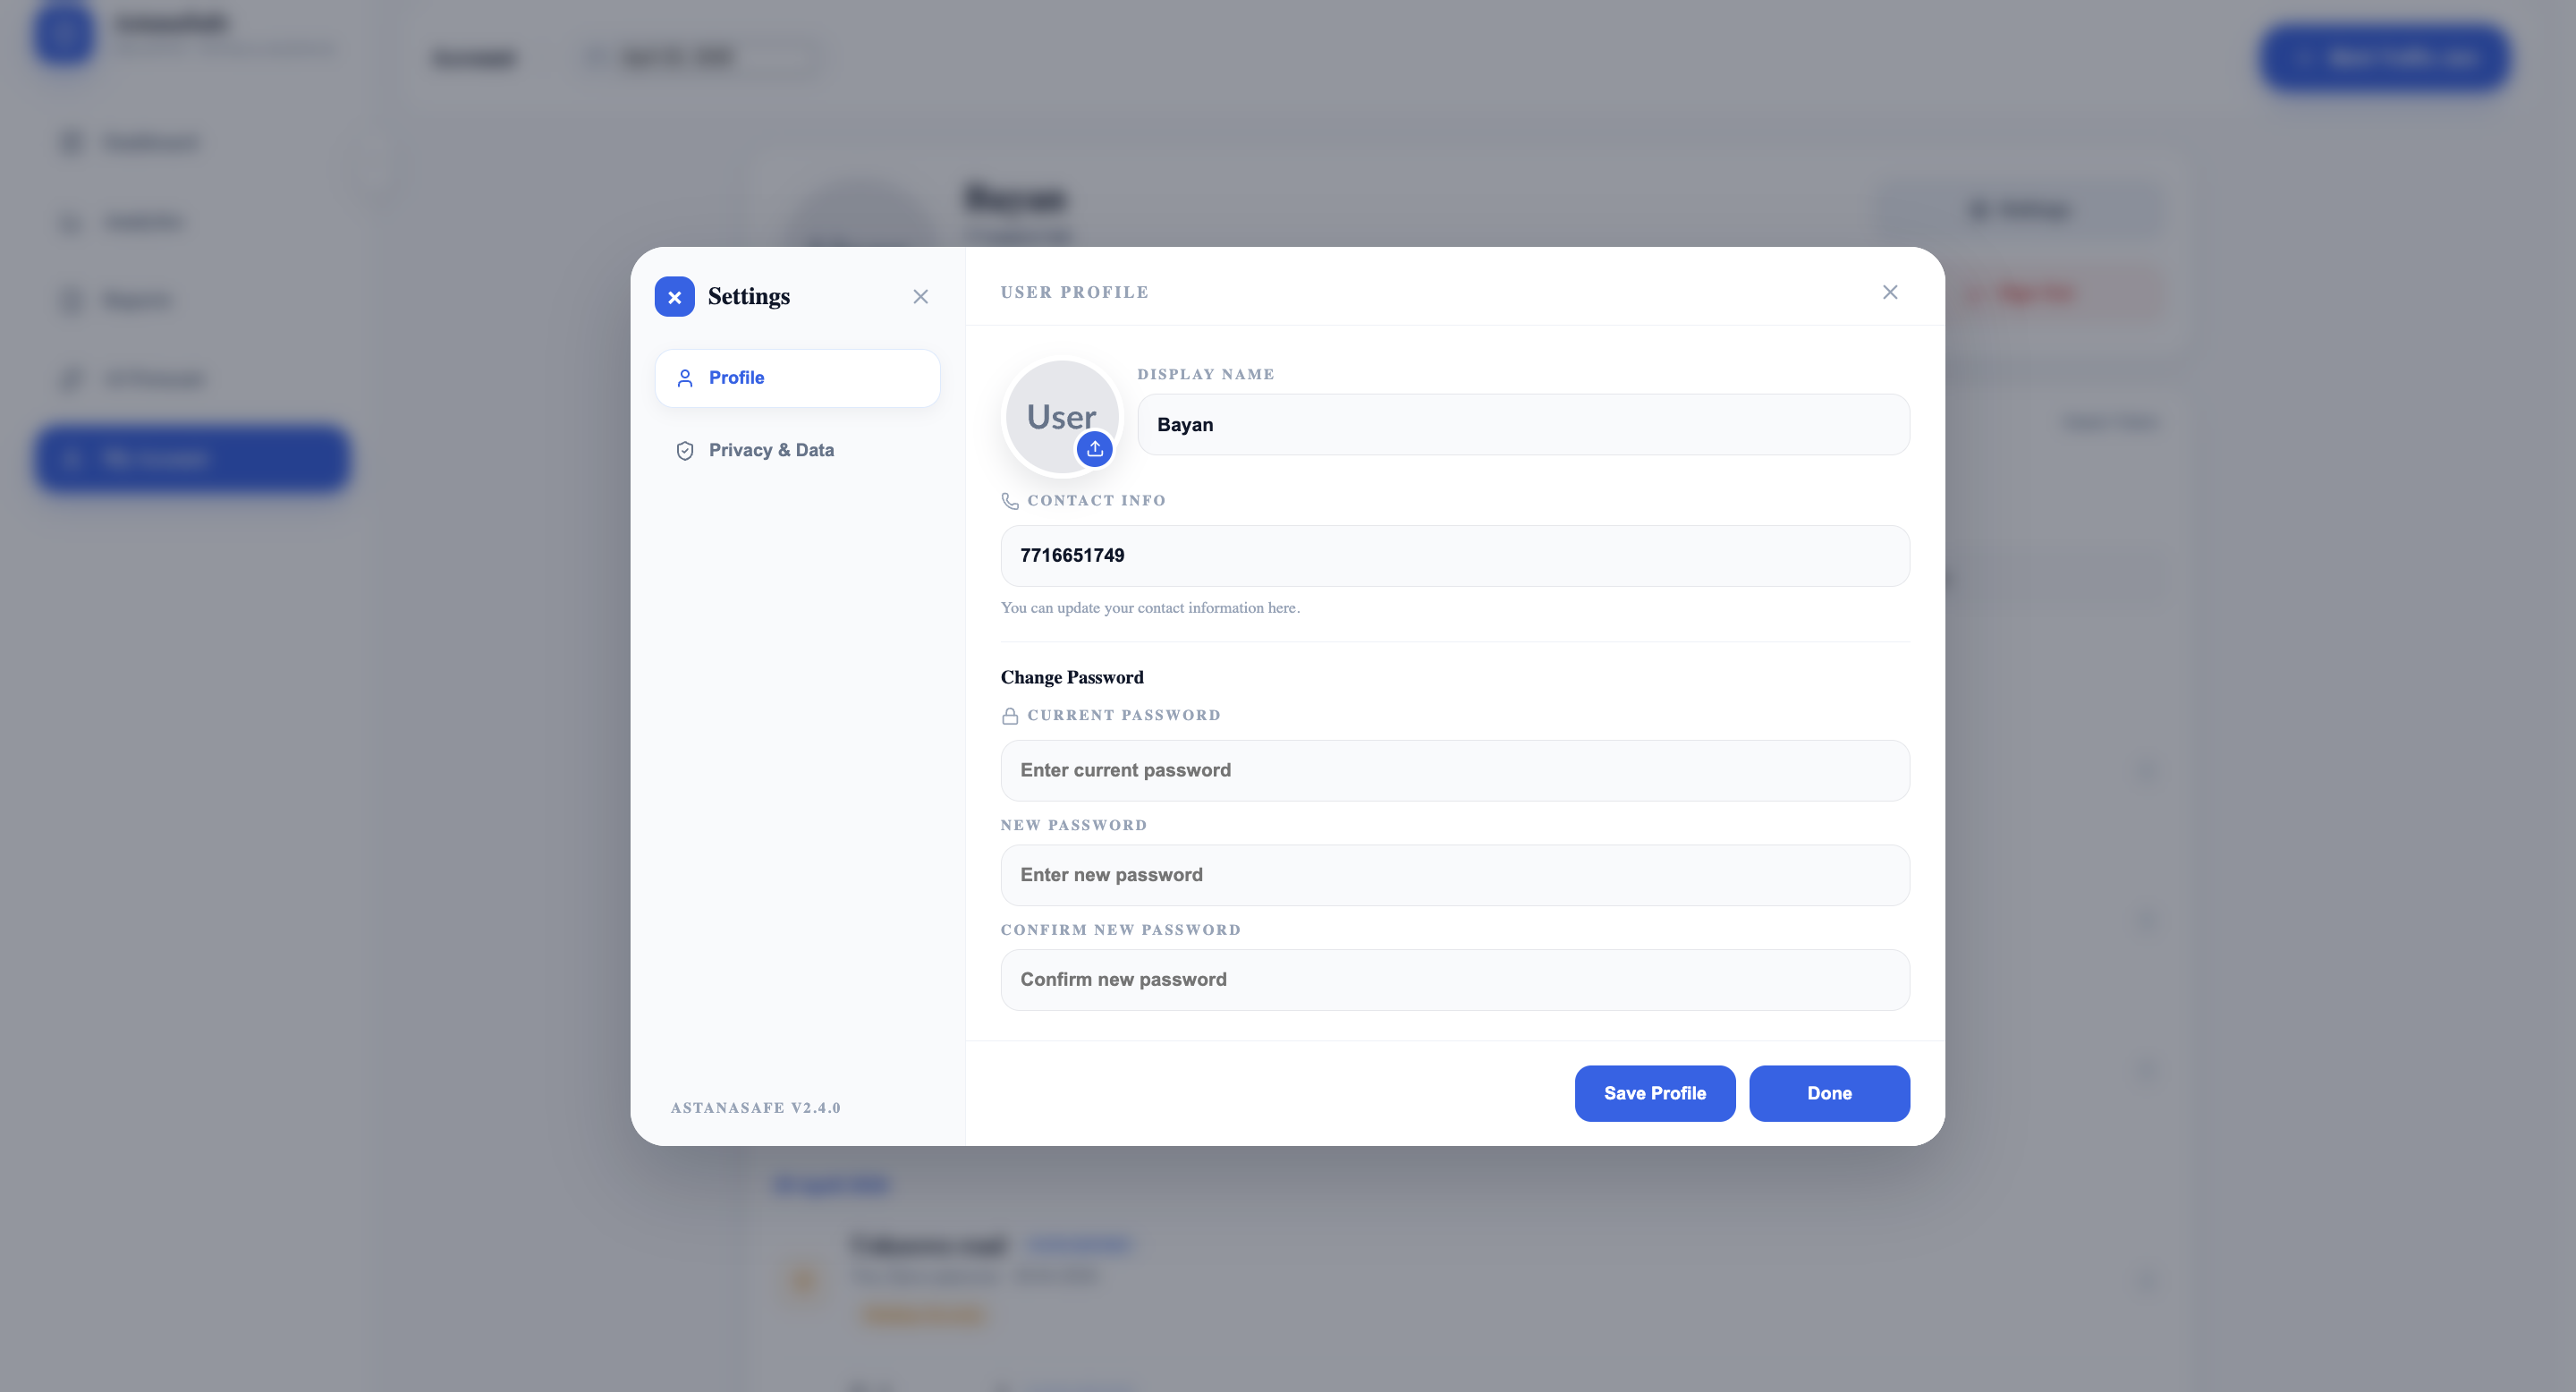
\includegraphics[width=0.82\textwidth]{sc9_settings_profile}
  \caption{\centering Settings modal - Profile tab: display name editor,
           contact information field, and the three-field change-password form
           (current password, new password, confirm new password)
           with Save Profile button.}
  \label{fig:app_settings_profile}
\end{figure}

\begin{figure}[H]
  \centering
  \addcontentsline{toc}{subsection}{Figure 15}
  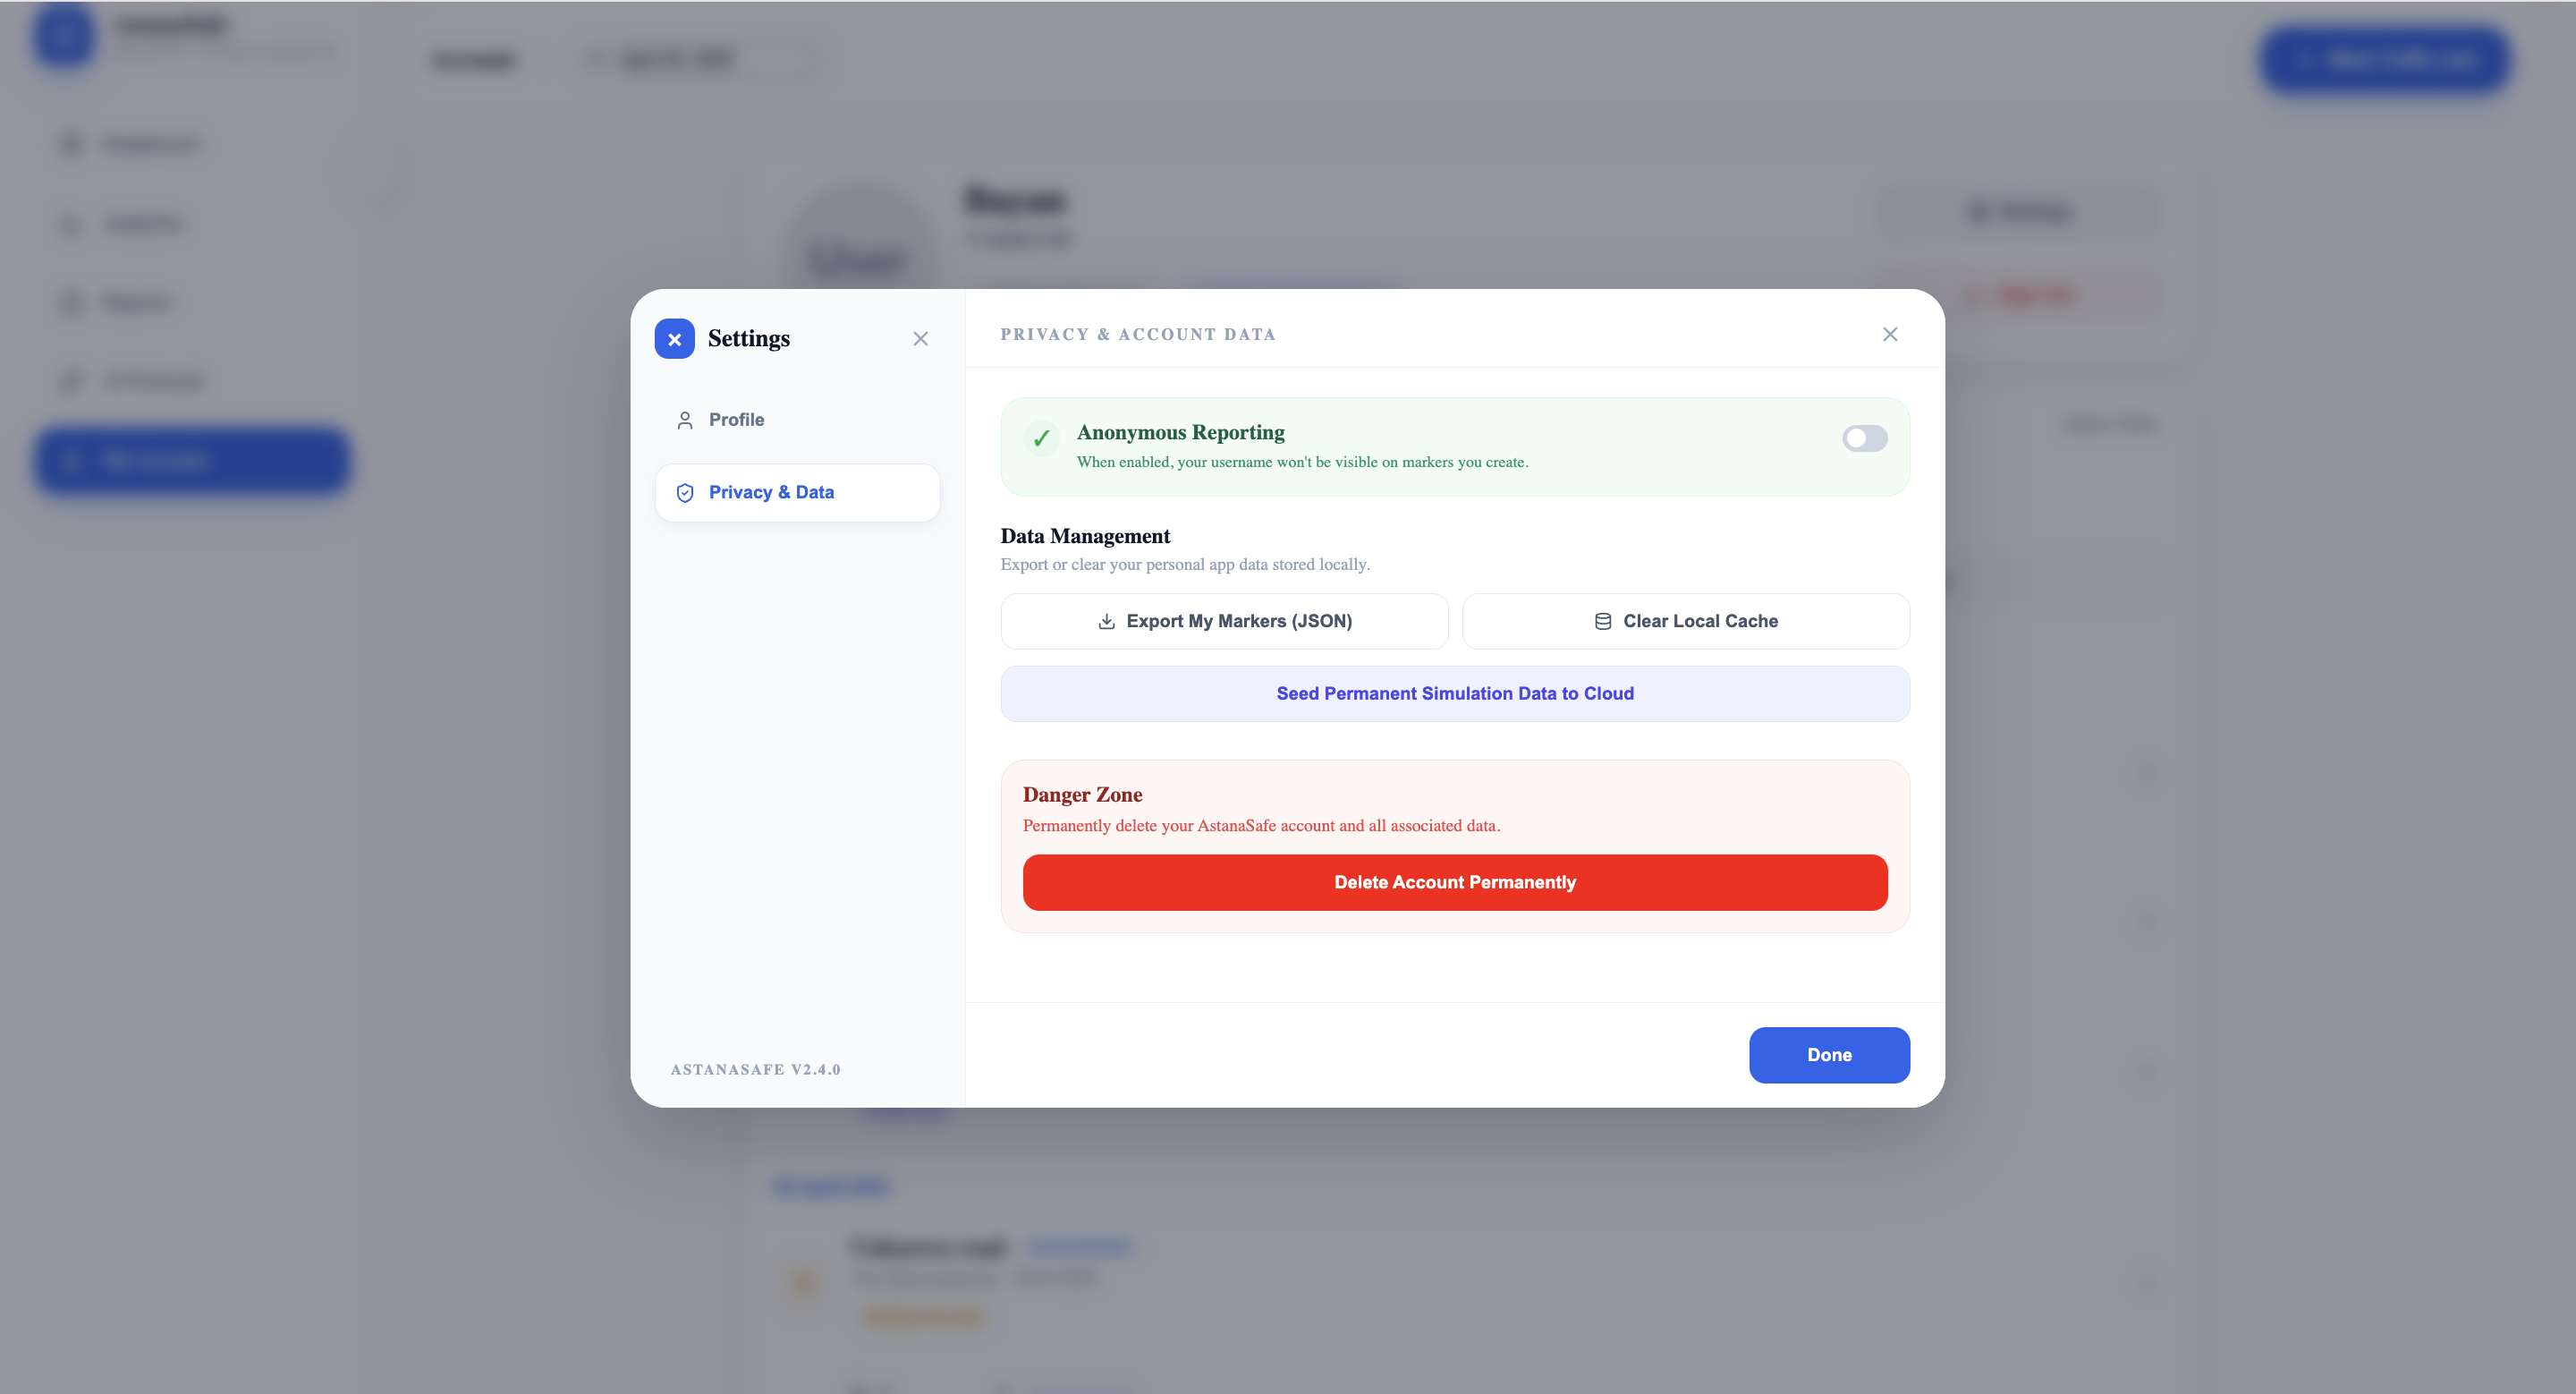
\includegraphics[width=0.82\textwidth]{sc10_settings_privacy}
  \caption{\centering Settings modal - Privacy \& Data tab: anonymous reporting
           toggle, data export (JSON) and cache clearing controls, and the
           permanent account deletion option in the Danger Zone section.}
  \label{fig:app_settings_privacy}
\end{figure}
\end{document}
